% Build with: make -C sparse_learning/slides
% All illustrations are editable TikZ/PGFPlots; no raster assets are required.
\documentclass[aspectratio=169,10pt]{beamer}
\title{Sparse Direct Solvers: Algorithms and Code}
\subtitle{Sparse LU factorization and a SuperLU-inspired Python implementation}
\usepackage[T1]{fontenc}
\usepackage{lmodern}
\usepackage{amsmath,amssymb,booktabs,listings,tikz,pgfplots}
\usetikzlibrary{arrows.meta,positioning,matrix,fit,calc,backgrounds,shapes.geometric}
\pgfplotsset{compat=1.18}

\definecolor{Navy}{HTML}{152B43}
\definecolor{Teal}{HTML}{087F8C}
\definecolor{Amber}{HTML}{D78B16}
\definecolor{Slate}{HTML}{526577}
\definecolor{Mist}{HTML}{F0F5F8}
\definecolor{Red}{HTML}{BC4653}
\setbeamercolor{normal text}{fg=Navy,bg=white}
\setbeamercolor{frametitle}{fg=Navy,bg=white}
\setbeamercolor{structure}{fg=Teal}
\setbeamercolor{block title}{fg=white,bg=Teal}
\setbeamercolor{block body}{fg=Navy,bg=Mist}
\setbeamerfont{frametitle}{size=\Large,series=\bfseries}
\setbeamertemplate{navigation symbols}{}
\setbeamertemplate{itemize item}{\color{Teal}\small$\bullet$}
\setbeamertemplate{footline}{%
  \hbox{\begin{beamercolorbox}[wd=.82\paperwidth,ht=3.2ex,dp=1.1ex,leftskip=.65cm]{normal text}
  \color{Slate}\scriptsize SPARSE LU \hspace{1em} Algorithms, implementation, and SuperLU
  \end{beamercolorbox}%
  \begin{beamercolorbox}[wd=.18\paperwidth,ht=3.2ex,dp=1.1ex,rightskip=.65cm plus1fil]{normal text}
  \hfill\color{Slate}\scriptsize\insertframenumber\,/\,\inserttotalframenumber
  \end{beamercolorbox}}
}
\setbeamersize{text margin left=.65cm,text margin right=.65cm}
\hypersetup{colorlinks=true,urlcolor=Teal,linkcolor=Teal,
 pdftitle={Sparse Direct Solvers: Algorithms and Code},
 pdfsubject={Sparse LU algorithms, solver stages, code architecture, and verification}}
\lstset{language=Python,basicstyle=\ttfamily\scriptsize,
 keywordstyle=\color{Teal}\bfseries,commentstyle=\color{Slate},
 stringstyle=\color{Amber!80!black},backgroundcolor=\color{Mist},
 showstringspaces=false,columns=fullflexible,keepspaces=true,
 breaklines=true,frame=none,xleftmargin=5pt,xrightmargin=5pt,
 aboveskip=5pt,belowskip=5pt}
\tikzset{
 flow/.style={draw=Teal!45,fill=Mist,rounded corners=3pt,align=center,
              minimum height=.65cm,font=\small,inner sep=6pt},
 vertex/.style={circle,draw=Teal,fill=Teal!10,minimum size=.52cm,inner sep=0pt,font=\small},
 faint/.style={circle,draw=Slate!35,fill=Mist,text=Slate,minimum size=.52cm,inner sep=0pt,font=\small},
 arr/.style={-{Stealth[length=2.2mm]},thick,draw=Teal},
 edge/.style={thick,draw=Slate!70},
 fillEdge/.style={thick,dashed,draw=Amber},
}

\newcommand{\takeaway}[1]{\vfill\begin{beamercolorbox}[sep=7pt,wd=\textwidth]{block body}\small\textbf{Key idea:} #1\end{beamercolorbox}}
\newcommand{\source}[1]{{\scriptsize\color{Slate}Source guide: \texttt{#1}}}
\newcommand{\numatrix}[3]{%
\begin{tikzpicture}[baseline=(M.center)]
\matrix (M) [matrix of math nodes,ampersand replacement=\&,
             nodes={minimum width=.59cm,minimum height=.52cm,inner sep=2pt},
             left delimiter={[},right delimiter={]}] {#1};
\begin{scope}[on background layer]
\if\relax\detokenize{#2}\relax\else
\foreach \r/\c in {#2}{\fill[Teal!14] (M-\r-\c.south west) rectangle (M-\r-\c.north east);}
\fi
\if\relax\detokenize{#3}\relax\else
\foreach \r/\c in {#3}{\fill[Amber!22] (M-\r-\c.south west) rectangle (M-\r-\c.north east);}
\fi
\end{scope}
\end{tikzpicture}}
\newcommand{\arrayrow}[3]{%
\node[anchor=east,font=\ttfamily\small,text=Slate] at (-.25,#1) {#2};
\foreach \value [count=\i from 0] in {#3}{
 \node[draw=Slate!30,fill=Mist,minimum width=.59cm,minimum height=.48cm,font=\ttfamily\small]
 at (.64*\i,#1) {\value};}}
\newcommand{\NaturalLNNZ}{519}
\newcommand{\NaturalUNNZ}{519}
\newcommand{\OrderedLNNZ}{411}
\newcommand{\OrderedUNNZ}{411}
\newcommand{\InputNNZ}{288}
\newcommand{\NaturalCombinedNNZ}{974}
\newcommand{\OrderedCombinedNNZ}{758}
\newcommand{\RefinementSteps}{1}


\begin{document}

% Slide 01 -------------------------------------------------------------
\begin{frame}[plain]
\vspace{.2cm}
{\color{Teal}\large NUMERICAL LINEAR ALGEBRA}\par\vspace{.25cm}
{\fontsize{27}{31}\selectfont\bfseries Sparse Direct Solvers\\Algorithms and Code}\par
\vspace{.25cm}
{\large Sparse LU factorization, structural analysis,\\and a Python implementation inspired by SuperLU.}
\vspace{.5cm}
\begin{columns}[c,onlytextwidth]
\column{.43\textwidth}\centering
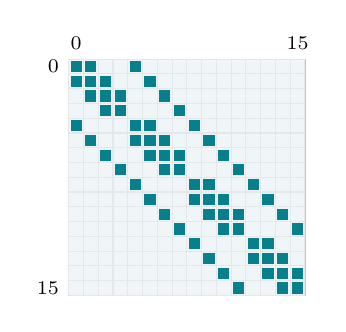
\begin{tikzpicture}[x=0.187500cm,y=0.187500cm]
\fill[Mist] (0,0) rectangle (16,-16);
\fill[Teal] (0.120,-0.120) rectangle (0.880,-0.880);
\fill[Teal] (1.120,-0.120) rectangle (1.880,-0.880);
\fill[Teal] (4.120,-0.120) rectangle (4.880,-0.880);
\fill[Teal] (0.120,-1.120) rectangle (0.880,-1.880);
\fill[Teal] (1.120,-1.120) rectangle (1.880,-1.880);
\fill[Teal] (2.120,-1.120) rectangle (2.880,-1.880);
\fill[Teal] (5.120,-1.120) rectangle (5.880,-1.880);
\fill[Teal] (1.120,-2.120) rectangle (1.880,-2.880);
\fill[Teal] (2.120,-2.120) rectangle (2.880,-2.880);
\fill[Teal] (3.120,-2.120) rectangle (3.880,-2.880);
\fill[Teal] (6.120,-2.120) rectangle (6.880,-2.880);
\fill[Teal] (2.120,-3.120) rectangle (2.880,-3.880);
\fill[Teal] (3.120,-3.120) rectangle (3.880,-3.880);
\fill[Teal] (7.120,-3.120) rectangle (7.880,-3.880);
\fill[Teal] (0.120,-4.120) rectangle (0.880,-4.880);
\fill[Teal] (4.120,-4.120) rectangle (4.880,-4.880);
\fill[Teal] (5.120,-4.120) rectangle (5.880,-4.880);
\fill[Teal] (8.120,-4.120) rectangle (8.880,-4.880);
\fill[Teal] (1.120,-5.120) rectangle (1.880,-5.880);
\fill[Teal] (4.120,-5.120) rectangle (4.880,-5.880);
\fill[Teal] (5.120,-5.120) rectangle (5.880,-5.880);
\fill[Teal] (6.120,-5.120) rectangle (6.880,-5.880);
\fill[Teal] (9.120,-5.120) rectangle (9.880,-5.880);
\fill[Teal] (2.120,-6.120) rectangle (2.880,-6.880);
\fill[Teal] (5.120,-6.120) rectangle (5.880,-6.880);
\fill[Teal] (6.120,-6.120) rectangle (6.880,-6.880);
\fill[Teal] (7.120,-6.120) rectangle (7.880,-6.880);
\fill[Teal] (10.120,-6.120) rectangle (10.880,-6.880);
\fill[Teal] (3.120,-7.120) rectangle (3.880,-7.880);
\fill[Teal] (6.120,-7.120) rectangle (6.880,-7.880);
\fill[Teal] (7.120,-7.120) rectangle (7.880,-7.880);
\fill[Teal] (11.120,-7.120) rectangle (11.880,-7.880);
\fill[Teal] (4.120,-8.120) rectangle (4.880,-8.880);
\fill[Teal] (8.120,-8.120) rectangle (8.880,-8.880);
\fill[Teal] (9.120,-8.120) rectangle (9.880,-8.880);
\fill[Teal] (12.120,-8.120) rectangle (12.880,-8.880);
\fill[Teal] (5.120,-9.120) rectangle (5.880,-9.880);
\fill[Teal] (8.120,-9.120) rectangle (8.880,-9.880);
\fill[Teal] (9.120,-9.120) rectangle (9.880,-9.880);
\fill[Teal] (10.120,-9.120) rectangle (10.880,-9.880);
\fill[Teal] (13.120,-9.120) rectangle (13.880,-9.880);
\fill[Teal] (6.120,-10.120) rectangle (6.880,-10.880);
\fill[Teal] (9.120,-10.120) rectangle (9.880,-10.880);
\fill[Teal] (10.120,-10.120) rectangle (10.880,-10.880);
\fill[Teal] (11.120,-10.120) rectangle (11.880,-10.880);
\fill[Teal] (14.120,-10.120) rectangle (14.880,-10.880);
\fill[Teal] (7.120,-11.120) rectangle (7.880,-11.880);
\fill[Teal] (10.120,-11.120) rectangle (10.880,-11.880);
\fill[Teal] (11.120,-11.120) rectangle (11.880,-11.880);
\fill[Teal] (15.120,-11.120) rectangle (15.880,-11.880);
\fill[Teal] (8.120,-12.120) rectangle (8.880,-12.880);
\fill[Teal] (12.120,-12.120) rectangle (12.880,-12.880);
\fill[Teal] (13.120,-12.120) rectangle (13.880,-12.880);
\fill[Teal] (9.120,-13.120) rectangle (9.880,-13.880);
\fill[Teal] (12.120,-13.120) rectangle (12.880,-13.880);
\fill[Teal] (13.120,-13.120) rectangle (13.880,-13.880);
\fill[Teal] (14.120,-13.120) rectangle (14.880,-13.880);
\fill[Teal] (10.120,-14.120) rectangle (10.880,-14.880);
\fill[Teal] (13.120,-14.120) rectangle (13.880,-14.880);
\fill[Teal] (14.120,-14.120) rectangle (14.880,-14.880);
\fill[Teal] (15.120,-14.120) rectangle (15.880,-14.880);
\fill[Teal] (11.120,-15.120) rectangle (11.880,-15.880);
\fill[Teal] (14.120,-15.120) rectangle (14.880,-15.880);
\fill[Teal] (15.120,-15.120) rectangle (15.880,-15.880);
\draw[Slate!35] (0,0) rectangle (16,-16);
\draw[Slate!15,step=1] (0,0) grid (16,-16);
\node[anchor=south,font=\scriptsize] at (.5,0) {0};
\node[anchor=south,font=\scriptsize] at (15.5,0) {15};
\node[anchor=east,font=\scriptsize] at (0,-.5) {0};
\node[anchor=east,font=\scriptsize] at (0,-15.5) {15};
\end{tikzpicture}
\par\small Sparse matrix $A$
\column{.12\textwidth}\centering

\begin{tikzpicture}\draw[arr,line width=1.4pt] (0,0)--(1.1,0);\end{tikzpicture}\par\small LU
\column{.43\textwidth}\centering
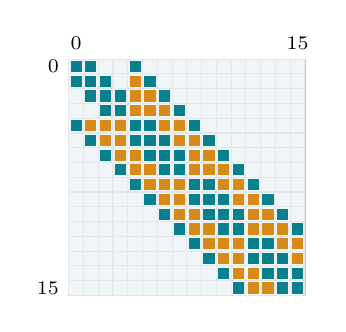
\begin{tikzpicture}[x=0.187500cm,y=0.187500cm]
\fill[Mist] (0,0) rectangle (16,-16);
\fill[Teal] (0.120,-0.120) rectangle (0.880,-0.880);
\fill[Teal] (1.120,-0.120) rectangle (1.880,-0.880);
\fill[Teal] (4.120,-0.120) rectangle (4.880,-0.880);
\fill[Teal] (0.120,-1.120) rectangle (0.880,-1.880);
\fill[Teal] (1.120,-1.120) rectangle (1.880,-1.880);
\fill[Teal] (2.120,-1.120) rectangle (2.880,-1.880);
\fill[Amber] (4.120,-1.120) rectangle (4.880,-1.880);
\fill[Teal] (5.120,-1.120) rectangle (5.880,-1.880);
\fill[Teal] (1.120,-2.120) rectangle (1.880,-2.880);
\fill[Teal] (2.120,-2.120) rectangle (2.880,-2.880);
\fill[Teal] (3.120,-2.120) rectangle (3.880,-2.880);
\fill[Amber] (4.120,-2.120) rectangle (4.880,-2.880);
\fill[Amber] (5.120,-2.120) rectangle (5.880,-2.880);
\fill[Teal] (6.120,-2.120) rectangle (6.880,-2.880);
\fill[Teal] (2.120,-3.120) rectangle (2.880,-3.880);
\fill[Teal] (3.120,-3.120) rectangle (3.880,-3.880);
\fill[Amber] (4.120,-3.120) rectangle (4.880,-3.880);
\fill[Amber] (5.120,-3.120) rectangle (5.880,-3.880);
\fill[Amber] (6.120,-3.120) rectangle (6.880,-3.880);
\fill[Teal] (7.120,-3.120) rectangle (7.880,-3.880);
\fill[Teal] (0.120,-4.120) rectangle (0.880,-4.880);
\fill[Amber] (1.120,-4.120) rectangle (1.880,-4.880);
\fill[Amber] (2.120,-4.120) rectangle (2.880,-4.880);
\fill[Amber] (3.120,-4.120) rectangle (3.880,-4.880);
\fill[Teal] (4.120,-4.120) rectangle (4.880,-4.880);
\fill[Teal] (5.120,-4.120) rectangle (5.880,-4.880);
\fill[Amber] (6.120,-4.120) rectangle (6.880,-4.880);
\fill[Amber] (7.120,-4.120) rectangle (7.880,-4.880);
\fill[Teal] (8.120,-4.120) rectangle (8.880,-4.880);
\fill[Teal] (1.120,-5.120) rectangle (1.880,-5.880);
\fill[Amber] (2.120,-5.120) rectangle (2.880,-5.880);
\fill[Amber] (3.120,-5.120) rectangle (3.880,-5.880);
\fill[Teal] (4.120,-5.120) rectangle (4.880,-5.880);
\fill[Teal] (5.120,-5.120) rectangle (5.880,-5.880);
\fill[Teal] (6.120,-5.120) rectangle (6.880,-5.880);
\fill[Amber] (7.120,-5.120) rectangle (7.880,-5.880);
\fill[Amber] (8.120,-5.120) rectangle (8.880,-5.880);
\fill[Teal] (9.120,-5.120) rectangle (9.880,-5.880);
\fill[Teal] (2.120,-6.120) rectangle (2.880,-6.880);
\fill[Amber] (3.120,-6.120) rectangle (3.880,-6.880);
\fill[Amber] (4.120,-6.120) rectangle (4.880,-6.880);
\fill[Teal] (5.120,-6.120) rectangle (5.880,-6.880);
\fill[Teal] (6.120,-6.120) rectangle (6.880,-6.880);
\fill[Teal] (7.120,-6.120) rectangle (7.880,-6.880);
\fill[Amber] (8.120,-6.120) rectangle (8.880,-6.880);
\fill[Amber] (9.120,-6.120) rectangle (9.880,-6.880);
\fill[Teal] (10.120,-6.120) rectangle (10.880,-6.880);
\fill[Teal] (3.120,-7.120) rectangle (3.880,-7.880);
\fill[Amber] (4.120,-7.120) rectangle (4.880,-7.880);
\fill[Amber] (5.120,-7.120) rectangle (5.880,-7.880);
\fill[Teal] (6.120,-7.120) rectangle (6.880,-7.880);
\fill[Teal] (7.120,-7.120) rectangle (7.880,-7.880);
\fill[Amber] (8.120,-7.120) rectangle (8.880,-7.880);
\fill[Amber] (9.120,-7.120) rectangle (9.880,-7.880);
\fill[Amber] (10.120,-7.120) rectangle (10.880,-7.880);
\fill[Teal] (11.120,-7.120) rectangle (11.880,-7.880);
\fill[Teal] (4.120,-8.120) rectangle (4.880,-8.880);
\fill[Amber] (5.120,-8.120) rectangle (5.880,-8.880);
\fill[Amber] (6.120,-8.120) rectangle (6.880,-8.880);
\fill[Amber] (7.120,-8.120) rectangle (7.880,-8.880);
\fill[Teal] (8.120,-8.120) rectangle (8.880,-8.880);
\fill[Teal] (9.120,-8.120) rectangle (9.880,-8.880);
\fill[Amber] (10.120,-8.120) rectangle (10.880,-8.880);
\fill[Amber] (11.120,-8.120) rectangle (11.880,-8.880);
\fill[Teal] (12.120,-8.120) rectangle (12.880,-8.880);
\fill[Teal] (5.120,-9.120) rectangle (5.880,-9.880);
\fill[Amber] (6.120,-9.120) rectangle (6.880,-9.880);
\fill[Amber] (7.120,-9.120) rectangle (7.880,-9.880);
\fill[Teal] (8.120,-9.120) rectangle (8.880,-9.880);
\fill[Teal] (9.120,-9.120) rectangle (9.880,-9.880);
\fill[Teal] (10.120,-9.120) rectangle (10.880,-9.880);
\fill[Amber] (11.120,-9.120) rectangle (11.880,-9.880);
\fill[Amber] (12.120,-9.120) rectangle (12.880,-9.880);
\fill[Teal] (13.120,-9.120) rectangle (13.880,-9.880);
\fill[Teal] (6.120,-10.120) rectangle (6.880,-10.880);
\fill[Amber] (7.120,-10.120) rectangle (7.880,-10.880);
\fill[Amber] (8.120,-10.120) rectangle (8.880,-10.880);
\fill[Teal] (9.120,-10.120) rectangle (9.880,-10.880);
\fill[Teal] (10.120,-10.120) rectangle (10.880,-10.880);
\fill[Teal] (11.120,-10.120) rectangle (11.880,-10.880);
\fill[Amber] (12.120,-10.120) rectangle (12.880,-10.880);
\fill[Amber] (13.120,-10.120) rectangle (13.880,-10.880);
\fill[Teal] (14.120,-10.120) rectangle (14.880,-10.880);
\fill[Teal] (7.120,-11.120) rectangle (7.880,-11.880);
\fill[Amber] (8.120,-11.120) rectangle (8.880,-11.880);
\fill[Amber] (9.120,-11.120) rectangle (9.880,-11.880);
\fill[Teal] (10.120,-11.120) rectangle (10.880,-11.880);
\fill[Teal] (11.120,-11.120) rectangle (11.880,-11.880);
\fill[Amber] (12.120,-11.120) rectangle (12.880,-11.880);
\fill[Amber] (13.120,-11.120) rectangle (13.880,-11.880);
\fill[Amber] (14.120,-11.120) rectangle (14.880,-11.880);
\fill[Teal] (15.120,-11.120) rectangle (15.880,-11.880);
\fill[Teal] (8.120,-12.120) rectangle (8.880,-12.880);
\fill[Amber] (9.120,-12.120) rectangle (9.880,-12.880);
\fill[Amber] (10.120,-12.120) rectangle (10.880,-12.880);
\fill[Amber] (11.120,-12.120) rectangle (11.880,-12.880);
\fill[Teal] (12.120,-12.120) rectangle (12.880,-12.880);
\fill[Teal] (13.120,-12.120) rectangle (13.880,-12.880);
\fill[Amber] (14.120,-12.120) rectangle (14.880,-12.880);
\fill[Amber] (15.120,-12.120) rectangle (15.880,-12.880);
\fill[Teal] (9.120,-13.120) rectangle (9.880,-13.880);
\fill[Amber] (10.120,-13.120) rectangle (10.880,-13.880);
\fill[Amber] (11.120,-13.120) rectangle (11.880,-13.880);
\fill[Teal] (12.120,-13.120) rectangle (12.880,-13.880);
\fill[Teal] (13.120,-13.120) rectangle (13.880,-13.880);
\fill[Teal] (14.120,-13.120) rectangle (14.880,-13.880);
\fill[Amber] (15.120,-13.120) rectangle (15.880,-13.880);
\fill[Teal] (10.120,-14.120) rectangle (10.880,-14.880);
\fill[Amber] (11.120,-14.120) rectangle (11.880,-14.880);
\fill[Amber] (12.120,-14.120) rectangle (12.880,-14.880);
\fill[Teal] (13.120,-14.120) rectangle (13.880,-14.880);
\fill[Teal] (14.120,-14.120) rectangle (14.880,-14.880);
\fill[Teal] (15.120,-14.120) rectangle (15.880,-14.880);
\fill[Teal] (11.120,-15.120) rectangle (11.880,-15.880);
\fill[Amber] (12.120,-15.120) rectangle (12.880,-15.880);
\fill[Amber] (13.120,-15.120) rectangle (13.880,-15.880);
\fill[Teal] (14.120,-15.120) rectangle (14.880,-15.880);
\fill[Teal] (15.120,-15.120) rectangle (15.880,-15.880);
\draw[Slate!35] (0,0) rectangle (16,-16);
\draw[Slate!15,step=1] (0,0) grid (16,-16);
\node[anchor=south,font=\scriptsize] at (.5,0) {0};
\node[anchor=south,font=\scriptsize] at (15.5,0) {15};
\node[anchor=east,font=\scriptsize] at (0,-.5) {0};
\node[anchor=east,font=\scriptsize] at (0,-15.5) {15};
\end{tikzpicture}
\par\small Sparse factors $L,U$
\end{columns}
\vfill\scriptsize\color{Slate}An introduction to the mathematics, the solver pipeline, and the implementation. All figures are editable TikZ.
\end{frame}

% Slide 02 -------------------------------------------------------------
\begin{frame}{The task is to solve a sparse linear system accurately}
\[
\boxed{\quad Ax=b,\qquad A\in\mathbb{R}^{n\times n},\quad\mathrm{nnz}(A)\ll n^2.\quad}
\]
\begin{columns}[T,onlytextwidth]
\column{.47\textwidth}
\textbf{Sparse direct approach}
\begin{itemize}\setlength\itemsep{5pt}
\item Factor $A$ into triangular factors, with permutations as needed.
\item Solve with those factors for one or many right-hand sides.
\item Use residuals and error estimates to assess the result.
\end{itemize}
\column{.49\textwidth}
\textbf{What determines the cost?}
\begin{itemize}\setlength\itemsep{5pt}
\item Input nonzeros and their graph structure.
\item Fill-in created during factorization.
\item Pivoting, ordering, and block organization.
\end{itemize}
\end{columns}
\vspace{.15cm}
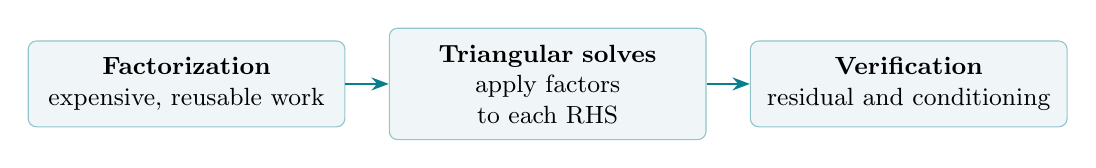
\begin{tikzpicture}[node distance=.55cm]
\node[flow,text width=3.6cm] (f) {\textbf{Factorization}\\expensive, reusable work};
\node[flow,text width=3.6cm,right=of f] (s) {\textbf{Triangular solves}\\apply factors to each RHS};
\node[flow,text width=3.6cm,right=of s] (v) {\textbf{Verification}\\residual and conditioning};
\draw[arr] (f)--(s);\draw[arr] (s)--(v);
\end{tikzpicture}
\takeaway{The code implements real-valued sparse LU. It supports nonsymmetric matrices; nonsingularity is required for a unique solution.}
\end{frame}

% Slide 03 -------------------------------------------------------------
\begin{frame}{SuperLU's driver separates preparation, factorization, and solve}
\centering
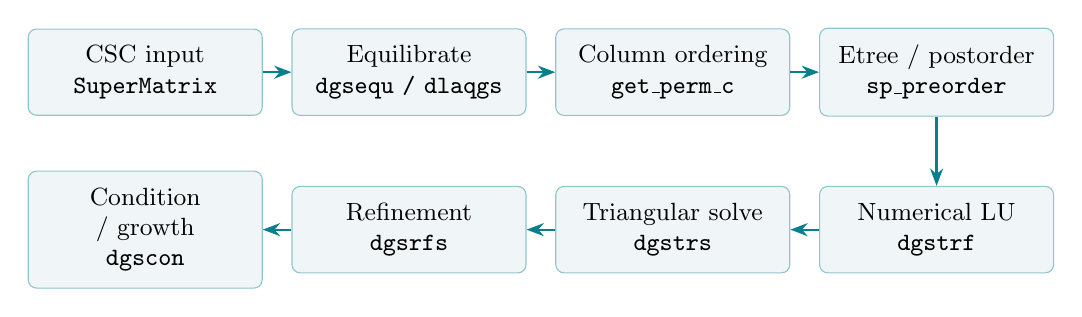
\begin{tikzpicture}
\node[flow,text width=2.55cm] (input) at (0,0) {CSC input\\\texttt{SuperMatrix}};
\node[flow,text width=2.55cm] (scale) at (3.35,0) {Equilibrate\\\texttt{dgsequ / dlaqgs}};
\node[flow,text width=2.55cm] (order) at (6.7,0) {Column ordering\\\texttt{get\_perm\_c}};
\node[flow,text width=2.55cm] (etree) at (10.05,0) {Etree / postorder\\\texttt{sp\_preorder}};
\node[flow,text width=2.55cm] (factor) at (10.05,-2.0) {Numerical LU\\\texttt{dgstrf}};
\node[flow,text width=2.55cm] (solve) at (6.7,-2.0) {Triangular solve\\\texttt{dgstrs}};
\node[flow,text width=2.55cm] (refine) at (3.35,-2.0) {Refinement\\\texttt{dgsrfs}};
\node[flow,text width=2.55cm] (diag) at (0,-2.0) {Condition / growth\\\texttt{dgscon}};
\draw[arr] (input)--(scale);\draw[arr] (scale)--(order);\draw[arr] (order)--(etree);
\draw[arr] (etree)--(factor);\draw[arr] (factor)--(solve);\draw[arr] (solve)--(refine);\draw[arr] (refine)--(diag);
\end{tikzpicture}\par
\vspace{.45cm}\small This is a learning sequence. The expert driver can compute condition and pivot-growth diagnostics before solving.
\par\vspace{.2cm}\source{superlu/SRC/dgssvx.c}
\takeaway{Use the driver to learn the stage boundaries before reading the inner numerical kernels.}
\end{frame}

% Slide 04 -------------------------------------------------------------
\begin{frame}{A scalar LU step stores a multiplier and updates a row}
\begin{columns}[c,onlytextwidth]
\column{.43\textwidth}\centering
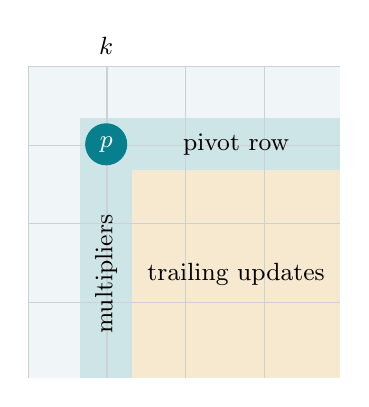
\begin{tikzpicture}[x=.66cm,y=.66cm]
\fill[Mist] (0,0) rectangle (6,-6);
\fill[Teal!20] (1,-1) rectangle (6,-2);
\fill[Teal!20] (1,-2) rectangle (2,-6);
\fill[Amber!20] (2,-2) rectangle (6,-6);
\draw[Slate!30] (0,0) grid (6,-6);
\node[vertex,fill=Teal,text=white] at (1.5,-1.5) {$p$};
\node[font=\small] at (4,-1.5) {pivot row};
\node[rotate=90,font=\small] at (1.5,-4) {multipliers};
\node[font=\small,align=center] at (4,-4) {trailing\ updates};
\node[font=\small] at (1.5,.4) {$k$};
\end{tikzpicture}
\column{.52\textwidth}
\textbf{For each row $i>k$ containing column $k$:}
\[
 l_{ik}=\frac{a_{ik}}{u_{kk}}
\]
\[
 a_{ij}\leftarrow a_{ij}-l_{ik}u_{kj},\qquad j>k.
\]
\begin{itemize}\setlength\itemsep{5pt}
\item Store $l_{ik}$ in $L$.
\item Remove the eliminated entry from the working row.
\item Insert new entries when the update creates fill.
\end{itemize}
\end{columns}
\takeaway{The division creates $L$; the row updates create $U$ and the evolving Schur complement.}
\end{frame}

% Slide 05 -------------------------------------------------------------
\begin{frame}{Eliminating one pivot can turn zeros into nonzeros}
\begin{columns}[c,onlytextwidth]
\column{.38\textwidth}\centering
\textbf{Before the first elimination}\par\vspace{.15cm}
\numatrix{4\&1\&1\\1\&4\&0\\1\&0\&4\\}{1/1,2/1,3/1}{2/3,3/2}
\column{.15\textwidth}\centering
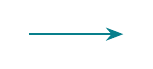
\begin{tikzpicture}\draw[arr] (0,0)--(1.2,0);\end{tikzpicture}\par\small $l_{10}=l_{20}=1/4$
\column{.40\textwidth}\centering
\textbf{Trailing block after elimination}\par\vspace{.15cm}
\numatrix{4\&1\&1\\0\&15/4\&-1/4\\0\&-1/4\&15/4\\}{1/1}{2/3,3/2}
\end{columns}
\vspace{.45cm}
\[
 a_{12}^{\mathrm{new}}=0-\left(\frac14\right)(1)=-\frac14,
 \qquad a_{21}^{\mathrm{new}}=-\frac14.
\]
\takeaway{These two orange entries are fill-in. Sparse input does not guarantee equally sparse factors.}
\end{frame}

% Slide 06 -------------------------------------------------------------
\begin{frame}{Partial pivoting selects a usable pivot row}
\begin{columns}[c,onlytextwidth]
\column{.30\textwidth}\centering
$A=$\numatrix{0\&2\&1\\1\&1\&0\\2\&0\&3\\}{3/1}{1/1}
\par\small The first diagonal is zero.
\column{.31\textwidth}\centering
\textbf{Swap rows 0 and 2}\par\vspace{.15cm}
\numatrix{2\&0\&3\\1\&1\&0\\0\&2\&1\\}{1/1,1/3}{}
\column{.31\textwidth}\centering
\textbf{Eliminate column 0}\par\vspace{.15cm}
\numatrix{2\&0\&3\\0\&1\&-3/2\\0\&2\&1\\}{1/1}{2/3}
\end{columns}
\vspace{.5cm}
\[
 p=2,\quad l_{10}=\frac12,\quad
 a_{12}^{\mathrm{new}}=0-\frac12(3)=-\frac32.
\]
\takeaway{Full partial pivoting chooses the largest magnitude in the active column. Threshold pivoting can prefer a sufficiently large original diagonal.}
\end{frame}

% Slide 07 -------------------------------------------------------------
\begin{frame}{A late row swap must also move previous multipliers}
\begin{columns}[c,onlytextwidth]
\column{.44\textwidth}\centering
\textbf{Before the second pivot}\par\vspace{.15cm}
$W=$\numatrix{2\&0\&3\\0\&1\&-3/2\\0\&2\&1\\}{3/2}{}
\par\vspace{.25cm}
Previous $L$ column:\quad$\begin{bmatrix}1&1/2&0\end{bmatrix}^{T}$
\column{.09\textwidth}\centering
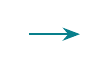
\begin{tikzpicture}\draw[arr] (0,0)--(.65,0);\end{tikzpicture}
\column{.44\textwidth}\centering
\textbf{Swap active rows 1 and 2}\par\vspace{.15cm}
$W=$\numatrix{2\&0\&3\\0\&2\&1\\0\&1\&-3/2\\}{2/2}{}
\par\vspace{.25cm}
Previous $L$ column:\quad$\begin{bmatrix}1&0&1/2\end{bmatrix}^{T}$
\end{columns}
\vspace{.4cm}
\centering\texttt{U[k], U[p] = U[p], U[k]}\par
\texttt{L[k], L[p] = L[p], L[k]}\par
\texttt{perm[k], perm[p] = perm[p], perm[k]}
\takeaway{The old multiplier belongs to an equation row. Moving that row must move its elimination history.}
\end{frame}

% Slide 08 -------------------------------------------------------------
\begin{frame}{The finished factors satisfy $PA=LU$}
\centering
\[
 PA=\begin{bmatrix}2&0&3\\0&2&1\\1&1&0\end{bmatrix},
 \qquad \texttt{perm}=[2,0,1].
\]
\vspace{.25cm}
\[
 L=\begin{bmatrix}1&0&0\\0&1&0\\1/2&1/2&1\end{bmatrix},
 \qquad
 U=\begin{bmatrix}2&0&3\\0&2&1\\0&0&-2\end{bmatrix}.
\]
\vspace{.3cm}
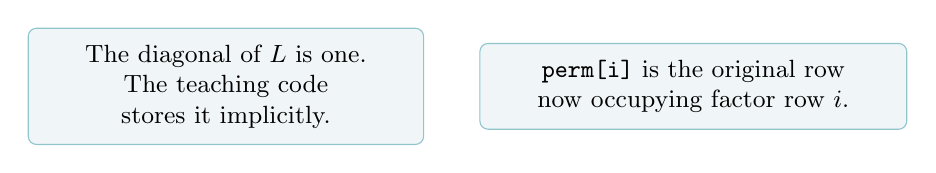
\begin{tikzpicture}
\node[flow,text width=4.6cm] (unit) {The diagonal of $L$ is one.\\The teaching code stores it implicitly.};
\node[flow,text width=5cm,right=.7cm of unit] {\texttt{perm[i]} is the original row\\now occupying factor row $i$.};
\end{tikzpicture}
\takeaway{Check the factorization identity independently. Correct-looking triangular factors are insufficient if the permutation is wrong.}
\end{frame}

% Slide 09 -------------------------------------------------------------
\begin{frame}{Solving uses the factors, not another elimination}
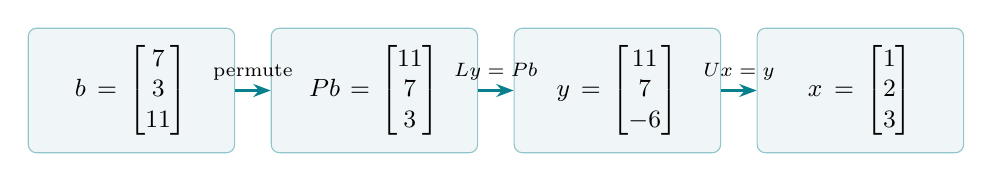
\begin{tikzpicture}[node distance=.45cm]
\node[flow,text width=2.2cm] (b) {$b=\begin{bmatrix}7\\3\\11\end{bmatrix}$};
\node[flow,text width=2.2cm,right=of b] (pb) {$Pb=\begin{bmatrix}11\\7\\3\end{bmatrix}$};
\node[flow,text width=2.2cm,right=of pb] (y) {$y=\begin{bmatrix}11\\7\\-6\end{bmatrix}$};
\node[flow,text width=2.2cm,right=of y] (x) {$x=\begin{bmatrix}1\\2\\3\end{bmatrix}$};
\draw[arr] (b)--node[above,font=\scriptsize]{permute}(pb);
\draw[arr] (pb)--node[above,font=\scriptsize]{$Ly=Pb$}(y);
\draw[arr] (y)--node[above,font=\scriptsize]{$Ux=y$}(x);
\end{tikzpicture}
\vspace{.55cm}
\begin{columns}[T,onlytextwidth]
\column{.47\textwidth}
\textbf{Forward substitution}
\[
 y_i=(Pb)_i-\sum_{j<i}l_{ij}y_j.
\]
\column{.47\textwidth}
\textbf{Backward substitution}
\[
 x_i=\frac{y_i-\sum_{j>i}u_{ij}x_j}{u_{ii}}.
\]
\end{columns}
\takeaway{Once $L,U,P$ exist, multiple right-hand sides reuse the same factorization.}
\end{frame}

% Slide 10 -------------------------------------------------------------
\begin{frame}{Equilibration balances row and column magnitudes}
\centering
\[
 A=\begin{bmatrix}2^{-10}&2^{-20}\\2^{10}&2^2\end{bmatrix},\quad
 R=\operatorname{diag}(2^{10},2^{-10}),\quad
 C=\operatorname{diag}(1,2^8).
\]
\vspace{.25cm}
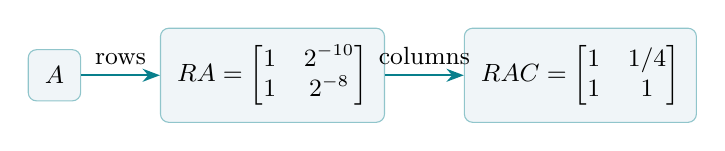
\begin{tikzpicture}
\node[flow] (a) {$A$};
\node[flow,right=1cm of a] (ra) {$RA=\begin{bmatrix}1&2^{-10}\\1&2^{-8}\end{bmatrix}$};
\node[flow,right=1cm of ra] (rac) {$RAC=\begin{bmatrix}1&1/4\\1&1\end{bmatrix}$};
\draw[arr] (a)--node[above,font=\small]{rows}(ra);\draw[arr] (ra)--node[above,font=\small]{columns}(rac);
\end{tikzpicture}\par
\vspace{.45cm}
\small Candidate row scales are inverse row maxima. Candidate column scales use the row-scaled matrix. Automatic selection uses scale ratios and safe magnitude limits; it need not apply both.
\par\vspace{.2cm}\source{dgsequ.c; dlaqgs.c}
\takeaway{Equilibration changes the numerical representation of the same linear problem. It does not remove singularity.}
\end{frame}

% Slide 11 -------------------------------------------------------------
\begin{frame}{Scaling and column ordering add two more maps}
\[
 \boxed{\;P_r\,(RAC)\,P_c=LU\;}
\]
\begin{columns}[T,onlytextwidth]
\column{.46\textwidth}
\textbf{Normal solve $Ax=b$}
\begin{align*}
 \widehat b &= P_r Rb,\\
 Ly &= \widehat b,\\
 Uz &= y,\\
 x &= CP_cz.
\end{align*}
\column{.50\textwidth}
\textbf{Conventions in the Python code}
\begin{itemize}\setlength\itemsep{5pt}
\item $R,C$: positive diagonal scales.
\item $p_k$: original row at factor row $k$.
\item $q_k$: original column at factor column $k$.
\item $\widehat b_k=R_{p_kp_k}b_{p_k}$.
\item $x_{q_k}=C_{q_kq_k}z_k$.
\end{itemize}
\small SuperLU's \texttt{perm\_r/perm\_c} arrays use the inverse, old-to-new convention.
\end{columns}
\takeaway{Row permutations reorder equations; column permutations reorder unknowns. Scaling must also be undone in the solution.}
\end{frame}

% Slide 12 -------------------------------------------------------------
\begin{frame}{Eliminating a high-degree vertex can create many fill edges}
\begin{columns}[c,onlytextwidth]
\column{.44\textwidth}\centering
\textbf{Eliminate the center first}\par\vspace{.2cm}
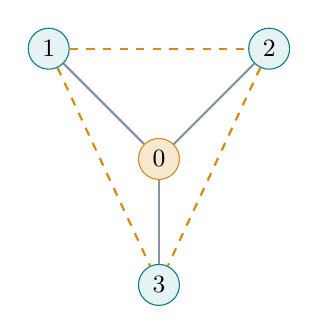
\begin{tikzpicture}
\node[vertex,fill=Amber!20,draw=Amber] (c) at (0,0) {0};
\node[vertex] (a) at (-1.4,1.4) {1};\node[vertex] (b) at (1.4,1.4) {2};\node[vertex] (d) at (0,-1.6) {3};
\draw[edge] (c)--(a);\draw[edge] (c)--(b);\draw[edge] (c)--(d);
\draw[fillEdge] (a)--(b);\draw[fillEdge] (a)--(d);\draw[fillEdge] (b)--(d);
\end{tikzpicture}
\par\small Its neighbors become a clique.
\column{.46\textwidth}\centering
\textbf{Eliminate a leaf first}\par\vspace{.2cm}
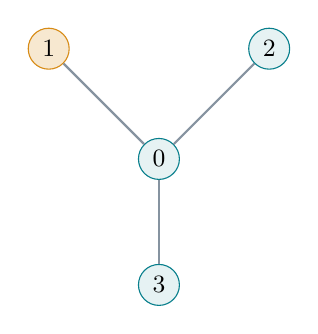
\begin{tikzpicture}
\node[vertex] (c) at (0,0) {0};
\node[vertex,fill=Amber!20,draw=Amber] (a) at (-1.4,1.4) {1};\node[vertex] (b) at (1.4,1.4) {2};\node[vertex] (d) at (0,-1.6) {3};
\draw[edge] (c)--(a);\draw[edge] (c)--(b);\draw[edge] (c)--(d);
\end{tikzpicture}
\par\small A single neighbor needs no fill edge.
\end{columns}
\takeaway{This graph-elimination illustration motivates minimum-degree ordering. Our code applies it to the structural column-intersection graph of $A^TA$.}
\end{frame}

% Slide 13 -------------------------------------------------------------
\begin{frame}{Ordering reduces factor storage on the same Poisson problem}
\begin{columns}[c,onlytextwidth]
\column{.32\textwidth}\centering
\textbf{Input $A$}\par\vspace{.1cm}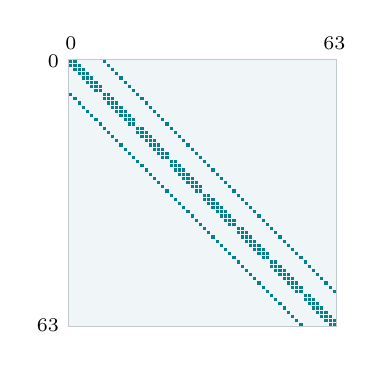
\begin{tikzpicture}[x=0.053125cm,y=0.053125cm]
\fill[Mist] (0,0) rectangle (64,-64);
\fill[Teal] (0.120,-0.120) rectangle (0.880,-0.880);
\fill[Teal] (1.120,-0.120) rectangle (1.880,-0.880);
\fill[Teal] (8.120,-0.120) rectangle (8.880,-0.880);
\fill[Teal] (0.120,-1.120) rectangle (0.880,-1.880);
\fill[Teal] (1.120,-1.120) rectangle (1.880,-1.880);
\fill[Teal] (2.120,-1.120) rectangle (2.880,-1.880);
\fill[Teal] (9.120,-1.120) rectangle (9.880,-1.880);
\fill[Teal] (1.120,-2.120) rectangle (1.880,-2.880);
\fill[Teal] (2.120,-2.120) rectangle (2.880,-2.880);
\fill[Teal] (3.120,-2.120) rectangle (3.880,-2.880);
\fill[Teal] (10.120,-2.120) rectangle (10.880,-2.880);
\fill[Teal] (2.120,-3.120) rectangle (2.880,-3.880);
\fill[Teal] (3.120,-3.120) rectangle (3.880,-3.880);
\fill[Teal] (4.120,-3.120) rectangle (4.880,-3.880);
\fill[Teal] (11.120,-3.120) rectangle (11.880,-3.880);
\fill[Teal] (3.120,-4.120) rectangle (3.880,-4.880);
\fill[Teal] (4.120,-4.120) rectangle (4.880,-4.880);
\fill[Teal] (5.120,-4.120) rectangle (5.880,-4.880);
\fill[Teal] (12.120,-4.120) rectangle (12.880,-4.880);
\fill[Teal] (4.120,-5.120) rectangle (4.880,-5.880);
\fill[Teal] (5.120,-5.120) rectangle (5.880,-5.880);
\fill[Teal] (6.120,-5.120) rectangle (6.880,-5.880);
\fill[Teal] (13.120,-5.120) rectangle (13.880,-5.880);
\fill[Teal] (5.120,-6.120) rectangle (5.880,-6.880);
\fill[Teal] (6.120,-6.120) rectangle (6.880,-6.880);
\fill[Teal] (7.120,-6.120) rectangle (7.880,-6.880);
\fill[Teal] (14.120,-6.120) rectangle (14.880,-6.880);
\fill[Teal] (6.120,-7.120) rectangle (6.880,-7.880);
\fill[Teal] (7.120,-7.120) rectangle (7.880,-7.880);
\fill[Teal] (15.120,-7.120) rectangle (15.880,-7.880);
\fill[Teal] (0.120,-8.120) rectangle (0.880,-8.880);
\fill[Teal] (8.120,-8.120) rectangle (8.880,-8.880);
\fill[Teal] (9.120,-8.120) rectangle (9.880,-8.880);
\fill[Teal] (16.120,-8.120) rectangle (16.880,-8.880);
\fill[Teal] (1.120,-9.120) rectangle (1.880,-9.880);
\fill[Teal] (8.120,-9.120) rectangle (8.880,-9.880);
\fill[Teal] (9.120,-9.120) rectangle (9.880,-9.880);
\fill[Teal] (10.120,-9.120) rectangle (10.880,-9.880);
\fill[Teal] (17.120,-9.120) rectangle (17.880,-9.880);
\fill[Teal] (2.120,-10.120) rectangle (2.880,-10.880);
\fill[Teal] (9.120,-10.120) rectangle (9.880,-10.880);
\fill[Teal] (10.120,-10.120) rectangle (10.880,-10.880);
\fill[Teal] (11.120,-10.120) rectangle (11.880,-10.880);
\fill[Teal] (18.120,-10.120) rectangle (18.880,-10.880);
\fill[Teal] (3.120,-11.120) rectangle (3.880,-11.880);
\fill[Teal] (10.120,-11.120) rectangle (10.880,-11.880);
\fill[Teal] (11.120,-11.120) rectangle (11.880,-11.880);
\fill[Teal] (12.120,-11.120) rectangle (12.880,-11.880);
\fill[Teal] (19.120,-11.120) rectangle (19.880,-11.880);
\fill[Teal] (4.120,-12.120) rectangle (4.880,-12.880);
\fill[Teal] (11.120,-12.120) rectangle (11.880,-12.880);
\fill[Teal] (12.120,-12.120) rectangle (12.880,-12.880);
\fill[Teal] (13.120,-12.120) rectangle (13.880,-12.880);
\fill[Teal] (20.120,-12.120) rectangle (20.880,-12.880);
\fill[Teal] (5.120,-13.120) rectangle (5.880,-13.880);
\fill[Teal] (12.120,-13.120) rectangle (12.880,-13.880);
\fill[Teal] (13.120,-13.120) rectangle (13.880,-13.880);
\fill[Teal] (14.120,-13.120) rectangle (14.880,-13.880);
\fill[Teal] (21.120,-13.120) rectangle (21.880,-13.880);
\fill[Teal] (6.120,-14.120) rectangle (6.880,-14.880);
\fill[Teal] (13.120,-14.120) rectangle (13.880,-14.880);
\fill[Teal] (14.120,-14.120) rectangle (14.880,-14.880);
\fill[Teal] (15.120,-14.120) rectangle (15.880,-14.880);
\fill[Teal] (22.120,-14.120) rectangle (22.880,-14.880);
\fill[Teal] (7.120,-15.120) rectangle (7.880,-15.880);
\fill[Teal] (14.120,-15.120) rectangle (14.880,-15.880);
\fill[Teal] (15.120,-15.120) rectangle (15.880,-15.880);
\fill[Teal] (23.120,-15.120) rectangle (23.880,-15.880);
\fill[Teal] (8.120,-16.120) rectangle (8.880,-16.880);
\fill[Teal] (16.120,-16.120) rectangle (16.880,-16.880);
\fill[Teal] (17.120,-16.120) rectangle (17.880,-16.880);
\fill[Teal] (24.120,-16.120) rectangle (24.880,-16.880);
\fill[Teal] (9.120,-17.120) rectangle (9.880,-17.880);
\fill[Teal] (16.120,-17.120) rectangle (16.880,-17.880);
\fill[Teal] (17.120,-17.120) rectangle (17.880,-17.880);
\fill[Teal] (18.120,-17.120) rectangle (18.880,-17.880);
\fill[Teal] (25.120,-17.120) rectangle (25.880,-17.880);
\fill[Teal] (10.120,-18.120) rectangle (10.880,-18.880);
\fill[Teal] (17.120,-18.120) rectangle (17.880,-18.880);
\fill[Teal] (18.120,-18.120) rectangle (18.880,-18.880);
\fill[Teal] (19.120,-18.120) rectangle (19.880,-18.880);
\fill[Teal] (26.120,-18.120) rectangle (26.880,-18.880);
\fill[Teal] (11.120,-19.120) rectangle (11.880,-19.880);
\fill[Teal] (18.120,-19.120) rectangle (18.880,-19.880);
\fill[Teal] (19.120,-19.120) rectangle (19.880,-19.880);
\fill[Teal] (20.120,-19.120) rectangle (20.880,-19.880);
\fill[Teal] (27.120,-19.120) rectangle (27.880,-19.880);
\fill[Teal] (12.120,-20.120) rectangle (12.880,-20.880);
\fill[Teal] (19.120,-20.120) rectangle (19.880,-20.880);
\fill[Teal] (20.120,-20.120) rectangle (20.880,-20.880);
\fill[Teal] (21.120,-20.120) rectangle (21.880,-20.880);
\fill[Teal] (28.120,-20.120) rectangle (28.880,-20.880);
\fill[Teal] (13.120,-21.120) rectangle (13.880,-21.880);
\fill[Teal] (20.120,-21.120) rectangle (20.880,-21.880);
\fill[Teal] (21.120,-21.120) rectangle (21.880,-21.880);
\fill[Teal] (22.120,-21.120) rectangle (22.880,-21.880);
\fill[Teal] (29.120,-21.120) rectangle (29.880,-21.880);
\fill[Teal] (14.120,-22.120) rectangle (14.880,-22.880);
\fill[Teal] (21.120,-22.120) rectangle (21.880,-22.880);
\fill[Teal] (22.120,-22.120) rectangle (22.880,-22.880);
\fill[Teal] (23.120,-22.120) rectangle (23.880,-22.880);
\fill[Teal] (30.120,-22.120) rectangle (30.880,-22.880);
\fill[Teal] (15.120,-23.120) rectangle (15.880,-23.880);
\fill[Teal] (22.120,-23.120) rectangle (22.880,-23.880);
\fill[Teal] (23.120,-23.120) rectangle (23.880,-23.880);
\fill[Teal] (31.120,-23.120) rectangle (31.880,-23.880);
\fill[Teal] (16.120,-24.120) rectangle (16.880,-24.880);
\fill[Teal] (24.120,-24.120) rectangle (24.880,-24.880);
\fill[Teal] (25.120,-24.120) rectangle (25.880,-24.880);
\fill[Teal] (32.120,-24.120) rectangle (32.880,-24.880);
\fill[Teal] (17.120,-25.120) rectangle (17.880,-25.880);
\fill[Teal] (24.120,-25.120) rectangle (24.880,-25.880);
\fill[Teal] (25.120,-25.120) rectangle (25.880,-25.880);
\fill[Teal] (26.120,-25.120) rectangle (26.880,-25.880);
\fill[Teal] (33.120,-25.120) rectangle (33.880,-25.880);
\fill[Teal] (18.120,-26.120) rectangle (18.880,-26.880);
\fill[Teal] (25.120,-26.120) rectangle (25.880,-26.880);
\fill[Teal] (26.120,-26.120) rectangle (26.880,-26.880);
\fill[Teal] (27.120,-26.120) rectangle (27.880,-26.880);
\fill[Teal] (34.120,-26.120) rectangle (34.880,-26.880);
\fill[Teal] (19.120,-27.120) rectangle (19.880,-27.880);
\fill[Teal] (26.120,-27.120) rectangle (26.880,-27.880);
\fill[Teal] (27.120,-27.120) rectangle (27.880,-27.880);
\fill[Teal] (28.120,-27.120) rectangle (28.880,-27.880);
\fill[Teal] (35.120,-27.120) rectangle (35.880,-27.880);
\fill[Teal] (20.120,-28.120) rectangle (20.880,-28.880);
\fill[Teal] (27.120,-28.120) rectangle (27.880,-28.880);
\fill[Teal] (28.120,-28.120) rectangle (28.880,-28.880);
\fill[Teal] (29.120,-28.120) rectangle (29.880,-28.880);
\fill[Teal] (36.120,-28.120) rectangle (36.880,-28.880);
\fill[Teal] (21.120,-29.120) rectangle (21.880,-29.880);
\fill[Teal] (28.120,-29.120) rectangle (28.880,-29.880);
\fill[Teal] (29.120,-29.120) rectangle (29.880,-29.880);
\fill[Teal] (30.120,-29.120) rectangle (30.880,-29.880);
\fill[Teal] (37.120,-29.120) rectangle (37.880,-29.880);
\fill[Teal] (22.120,-30.120) rectangle (22.880,-30.880);
\fill[Teal] (29.120,-30.120) rectangle (29.880,-30.880);
\fill[Teal] (30.120,-30.120) rectangle (30.880,-30.880);
\fill[Teal] (31.120,-30.120) rectangle (31.880,-30.880);
\fill[Teal] (38.120,-30.120) rectangle (38.880,-30.880);
\fill[Teal] (23.120,-31.120) rectangle (23.880,-31.880);
\fill[Teal] (30.120,-31.120) rectangle (30.880,-31.880);
\fill[Teal] (31.120,-31.120) rectangle (31.880,-31.880);
\fill[Teal] (39.120,-31.120) rectangle (39.880,-31.880);
\fill[Teal] (24.120,-32.120) rectangle (24.880,-32.880);
\fill[Teal] (32.120,-32.120) rectangle (32.880,-32.880);
\fill[Teal] (33.120,-32.120) rectangle (33.880,-32.880);
\fill[Teal] (40.120,-32.120) rectangle (40.880,-32.880);
\fill[Teal] (25.120,-33.120) rectangle (25.880,-33.880);
\fill[Teal] (32.120,-33.120) rectangle (32.880,-33.880);
\fill[Teal] (33.120,-33.120) rectangle (33.880,-33.880);
\fill[Teal] (34.120,-33.120) rectangle (34.880,-33.880);
\fill[Teal] (41.120,-33.120) rectangle (41.880,-33.880);
\fill[Teal] (26.120,-34.120) rectangle (26.880,-34.880);
\fill[Teal] (33.120,-34.120) rectangle (33.880,-34.880);
\fill[Teal] (34.120,-34.120) rectangle (34.880,-34.880);
\fill[Teal] (35.120,-34.120) rectangle (35.880,-34.880);
\fill[Teal] (42.120,-34.120) rectangle (42.880,-34.880);
\fill[Teal] (27.120,-35.120) rectangle (27.880,-35.880);
\fill[Teal] (34.120,-35.120) rectangle (34.880,-35.880);
\fill[Teal] (35.120,-35.120) rectangle (35.880,-35.880);
\fill[Teal] (36.120,-35.120) rectangle (36.880,-35.880);
\fill[Teal] (43.120,-35.120) rectangle (43.880,-35.880);
\fill[Teal] (28.120,-36.120) rectangle (28.880,-36.880);
\fill[Teal] (35.120,-36.120) rectangle (35.880,-36.880);
\fill[Teal] (36.120,-36.120) rectangle (36.880,-36.880);
\fill[Teal] (37.120,-36.120) rectangle (37.880,-36.880);
\fill[Teal] (44.120,-36.120) rectangle (44.880,-36.880);
\fill[Teal] (29.120,-37.120) rectangle (29.880,-37.880);
\fill[Teal] (36.120,-37.120) rectangle (36.880,-37.880);
\fill[Teal] (37.120,-37.120) rectangle (37.880,-37.880);
\fill[Teal] (38.120,-37.120) rectangle (38.880,-37.880);
\fill[Teal] (45.120,-37.120) rectangle (45.880,-37.880);
\fill[Teal] (30.120,-38.120) rectangle (30.880,-38.880);
\fill[Teal] (37.120,-38.120) rectangle (37.880,-38.880);
\fill[Teal] (38.120,-38.120) rectangle (38.880,-38.880);
\fill[Teal] (39.120,-38.120) rectangle (39.880,-38.880);
\fill[Teal] (46.120,-38.120) rectangle (46.880,-38.880);
\fill[Teal] (31.120,-39.120) rectangle (31.880,-39.880);
\fill[Teal] (38.120,-39.120) rectangle (38.880,-39.880);
\fill[Teal] (39.120,-39.120) rectangle (39.880,-39.880);
\fill[Teal] (47.120,-39.120) rectangle (47.880,-39.880);
\fill[Teal] (32.120,-40.120) rectangle (32.880,-40.880);
\fill[Teal] (40.120,-40.120) rectangle (40.880,-40.880);
\fill[Teal] (41.120,-40.120) rectangle (41.880,-40.880);
\fill[Teal] (48.120,-40.120) rectangle (48.880,-40.880);
\fill[Teal] (33.120,-41.120) rectangle (33.880,-41.880);
\fill[Teal] (40.120,-41.120) rectangle (40.880,-41.880);
\fill[Teal] (41.120,-41.120) rectangle (41.880,-41.880);
\fill[Teal] (42.120,-41.120) rectangle (42.880,-41.880);
\fill[Teal] (49.120,-41.120) rectangle (49.880,-41.880);
\fill[Teal] (34.120,-42.120) rectangle (34.880,-42.880);
\fill[Teal] (41.120,-42.120) rectangle (41.880,-42.880);
\fill[Teal] (42.120,-42.120) rectangle (42.880,-42.880);
\fill[Teal] (43.120,-42.120) rectangle (43.880,-42.880);
\fill[Teal] (50.120,-42.120) rectangle (50.880,-42.880);
\fill[Teal] (35.120,-43.120) rectangle (35.880,-43.880);
\fill[Teal] (42.120,-43.120) rectangle (42.880,-43.880);
\fill[Teal] (43.120,-43.120) rectangle (43.880,-43.880);
\fill[Teal] (44.120,-43.120) rectangle (44.880,-43.880);
\fill[Teal] (51.120,-43.120) rectangle (51.880,-43.880);
\fill[Teal] (36.120,-44.120) rectangle (36.880,-44.880);
\fill[Teal] (43.120,-44.120) rectangle (43.880,-44.880);
\fill[Teal] (44.120,-44.120) rectangle (44.880,-44.880);
\fill[Teal] (45.120,-44.120) rectangle (45.880,-44.880);
\fill[Teal] (52.120,-44.120) rectangle (52.880,-44.880);
\fill[Teal] (37.120,-45.120) rectangle (37.880,-45.880);
\fill[Teal] (44.120,-45.120) rectangle (44.880,-45.880);
\fill[Teal] (45.120,-45.120) rectangle (45.880,-45.880);
\fill[Teal] (46.120,-45.120) rectangle (46.880,-45.880);
\fill[Teal] (53.120,-45.120) rectangle (53.880,-45.880);
\fill[Teal] (38.120,-46.120) rectangle (38.880,-46.880);
\fill[Teal] (45.120,-46.120) rectangle (45.880,-46.880);
\fill[Teal] (46.120,-46.120) rectangle (46.880,-46.880);
\fill[Teal] (47.120,-46.120) rectangle (47.880,-46.880);
\fill[Teal] (54.120,-46.120) rectangle (54.880,-46.880);
\fill[Teal] (39.120,-47.120) rectangle (39.880,-47.880);
\fill[Teal] (46.120,-47.120) rectangle (46.880,-47.880);
\fill[Teal] (47.120,-47.120) rectangle (47.880,-47.880);
\fill[Teal] (55.120,-47.120) rectangle (55.880,-47.880);
\fill[Teal] (40.120,-48.120) rectangle (40.880,-48.880);
\fill[Teal] (48.120,-48.120) rectangle (48.880,-48.880);
\fill[Teal] (49.120,-48.120) rectangle (49.880,-48.880);
\fill[Teal] (56.120,-48.120) rectangle (56.880,-48.880);
\fill[Teal] (41.120,-49.120) rectangle (41.880,-49.880);
\fill[Teal] (48.120,-49.120) rectangle (48.880,-49.880);
\fill[Teal] (49.120,-49.120) rectangle (49.880,-49.880);
\fill[Teal] (50.120,-49.120) rectangle (50.880,-49.880);
\fill[Teal] (57.120,-49.120) rectangle (57.880,-49.880);
\fill[Teal] (42.120,-50.120) rectangle (42.880,-50.880);
\fill[Teal] (49.120,-50.120) rectangle (49.880,-50.880);
\fill[Teal] (50.120,-50.120) rectangle (50.880,-50.880);
\fill[Teal] (51.120,-50.120) rectangle (51.880,-50.880);
\fill[Teal] (58.120,-50.120) rectangle (58.880,-50.880);
\fill[Teal] (43.120,-51.120) rectangle (43.880,-51.880);
\fill[Teal] (50.120,-51.120) rectangle (50.880,-51.880);
\fill[Teal] (51.120,-51.120) rectangle (51.880,-51.880);
\fill[Teal] (52.120,-51.120) rectangle (52.880,-51.880);
\fill[Teal] (59.120,-51.120) rectangle (59.880,-51.880);
\fill[Teal] (44.120,-52.120) rectangle (44.880,-52.880);
\fill[Teal] (51.120,-52.120) rectangle (51.880,-52.880);
\fill[Teal] (52.120,-52.120) rectangle (52.880,-52.880);
\fill[Teal] (53.120,-52.120) rectangle (53.880,-52.880);
\fill[Teal] (60.120,-52.120) rectangle (60.880,-52.880);
\fill[Teal] (45.120,-53.120) rectangle (45.880,-53.880);
\fill[Teal] (52.120,-53.120) rectangle (52.880,-53.880);
\fill[Teal] (53.120,-53.120) rectangle (53.880,-53.880);
\fill[Teal] (54.120,-53.120) rectangle (54.880,-53.880);
\fill[Teal] (61.120,-53.120) rectangle (61.880,-53.880);
\fill[Teal] (46.120,-54.120) rectangle (46.880,-54.880);
\fill[Teal] (53.120,-54.120) rectangle (53.880,-54.880);
\fill[Teal] (54.120,-54.120) rectangle (54.880,-54.880);
\fill[Teal] (55.120,-54.120) rectangle (55.880,-54.880);
\fill[Teal] (62.120,-54.120) rectangle (62.880,-54.880);
\fill[Teal] (47.120,-55.120) rectangle (47.880,-55.880);
\fill[Teal] (54.120,-55.120) rectangle (54.880,-55.880);
\fill[Teal] (55.120,-55.120) rectangle (55.880,-55.880);
\fill[Teal] (63.120,-55.120) rectangle (63.880,-55.880);
\fill[Teal] (48.120,-56.120) rectangle (48.880,-56.880);
\fill[Teal] (56.120,-56.120) rectangle (56.880,-56.880);
\fill[Teal] (57.120,-56.120) rectangle (57.880,-56.880);
\fill[Teal] (49.120,-57.120) rectangle (49.880,-57.880);
\fill[Teal] (56.120,-57.120) rectangle (56.880,-57.880);
\fill[Teal] (57.120,-57.120) rectangle (57.880,-57.880);
\fill[Teal] (58.120,-57.120) rectangle (58.880,-57.880);
\fill[Teal] (50.120,-58.120) rectangle (50.880,-58.880);
\fill[Teal] (57.120,-58.120) rectangle (57.880,-58.880);
\fill[Teal] (58.120,-58.120) rectangle (58.880,-58.880);
\fill[Teal] (59.120,-58.120) rectangle (59.880,-58.880);
\fill[Teal] (51.120,-59.120) rectangle (51.880,-59.880);
\fill[Teal] (58.120,-59.120) rectangle (58.880,-59.880);
\fill[Teal] (59.120,-59.120) rectangle (59.880,-59.880);
\fill[Teal] (60.120,-59.120) rectangle (60.880,-59.880);
\fill[Teal] (52.120,-60.120) rectangle (52.880,-60.880);
\fill[Teal] (59.120,-60.120) rectangle (59.880,-60.880);
\fill[Teal] (60.120,-60.120) rectangle (60.880,-60.880);
\fill[Teal] (61.120,-60.120) rectangle (61.880,-60.880);
\fill[Teal] (53.120,-61.120) rectangle (53.880,-61.880);
\fill[Teal] (60.120,-61.120) rectangle (60.880,-61.880);
\fill[Teal] (61.120,-61.120) rectangle (61.880,-61.880);
\fill[Teal] (62.120,-61.120) rectangle (62.880,-61.880);
\fill[Teal] (54.120,-62.120) rectangle (54.880,-62.880);
\fill[Teal] (61.120,-62.120) rectangle (61.880,-62.880);
\fill[Teal] (62.120,-62.120) rectangle (62.880,-62.880);
\fill[Teal] (63.120,-62.120) rectangle (63.880,-62.880);
\fill[Teal] (55.120,-63.120) rectangle (55.880,-63.880);
\fill[Teal] (62.120,-63.120) rectangle (62.880,-63.880);
\fill[Teal] (63.120,-63.120) rectangle (63.880,-63.880);
\draw[Slate!35] (0,0) rectangle (64,-64);
\node[anchor=south,font=\scriptsize] at (.5,0) {0};
\node[anchor=south,font=\scriptsize] at (63.5,0) {63};
\node[anchor=east,font=\scriptsize] at (0,-.5) {0};
\node[anchor=east,font=\scriptsize] at (0,-63.5) {63};
\end{tikzpicture}

\par\small $64\times64$, $\mathrm{nnz}(A)=\InputNNZ$
\column{.32\textwidth}\centering
\textbf{Natural ordering}\par\vspace{.1cm}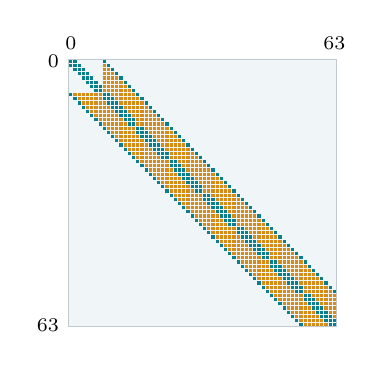
\begin{tikzpicture}[x=0.053125cm,y=0.053125cm]
\fill[Mist] (0,0) rectangle (64,-64);
\fill[Teal] (0.120,-0.120) rectangle (0.880,-0.880);
\fill[Teal] (1.120,-0.120) rectangle (1.880,-0.880);
\fill[Teal] (8.120,-0.120) rectangle (8.880,-0.880);
\fill[Teal] (0.120,-1.120) rectangle (0.880,-1.880);
\fill[Teal] (1.120,-1.120) rectangle (1.880,-1.880);
\fill[Teal] (2.120,-1.120) rectangle (2.880,-1.880);
\fill[Amber] (8.120,-1.120) rectangle (8.880,-1.880);
\fill[Teal] (9.120,-1.120) rectangle (9.880,-1.880);
\fill[Teal] (1.120,-2.120) rectangle (1.880,-2.880);
\fill[Teal] (2.120,-2.120) rectangle (2.880,-2.880);
\fill[Teal] (3.120,-2.120) rectangle (3.880,-2.880);
\fill[Amber] (8.120,-2.120) rectangle (8.880,-2.880);
\fill[Amber] (9.120,-2.120) rectangle (9.880,-2.880);
\fill[Teal] (10.120,-2.120) rectangle (10.880,-2.880);
\fill[Teal] (2.120,-3.120) rectangle (2.880,-3.880);
\fill[Teal] (3.120,-3.120) rectangle (3.880,-3.880);
\fill[Teal] (4.120,-3.120) rectangle (4.880,-3.880);
\fill[Amber] (8.120,-3.120) rectangle (8.880,-3.880);
\fill[Amber] (9.120,-3.120) rectangle (9.880,-3.880);
\fill[Amber] (10.120,-3.120) rectangle (10.880,-3.880);
\fill[Teal] (11.120,-3.120) rectangle (11.880,-3.880);
\fill[Teal] (3.120,-4.120) rectangle (3.880,-4.880);
\fill[Teal] (4.120,-4.120) rectangle (4.880,-4.880);
\fill[Teal] (5.120,-4.120) rectangle (5.880,-4.880);
\fill[Amber] (8.120,-4.120) rectangle (8.880,-4.880);
\fill[Amber] (9.120,-4.120) rectangle (9.880,-4.880);
\fill[Amber] (10.120,-4.120) rectangle (10.880,-4.880);
\fill[Amber] (11.120,-4.120) rectangle (11.880,-4.880);
\fill[Teal] (12.120,-4.120) rectangle (12.880,-4.880);
\fill[Teal] (4.120,-5.120) rectangle (4.880,-5.880);
\fill[Teal] (5.120,-5.120) rectangle (5.880,-5.880);
\fill[Teal] (6.120,-5.120) rectangle (6.880,-5.880);
\fill[Amber] (8.120,-5.120) rectangle (8.880,-5.880);
\fill[Amber] (9.120,-5.120) rectangle (9.880,-5.880);
\fill[Amber] (10.120,-5.120) rectangle (10.880,-5.880);
\fill[Amber] (11.120,-5.120) rectangle (11.880,-5.880);
\fill[Amber] (12.120,-5.120) rectangle (12.880,-5.880);
\fill[Teal] (13.120,-5.120) rectangle (13.880,-5.880);
\fill[Teal] (5.120,-6.120) rectangle (5.880,-6.880);
\fill[Teal] (6.120,-6.120) rectangle (6.880,-6.880);
\fill[Teal] (7.120,-6.120) rectangle (7.880,-6.880);
\fill[Amber] (8.120,-6.120) rectangle (8.880,-6.880);
\fill[Amber] (9.120,-6.120) rectangle (9.880,-6.880);
\fill[Amber] (10.120,-6.120) rectangle (10.880,-6.880);
\fill[Amber] (11.120,-6.120) rectangle (11.880,-6.880);
\fill[Amber] (12.120,-6.120) rectangle (12.880,-6.880);
\fill[Amber] (13.120,-6.120) rectangle (13.880,-6.880);
\fill[Teal] (14.120,-6.120) rectangle (14.880,-6.880);
\fill[Teal] (6.120,-7.120) rectangle (6.880,-7.880);
\fill[Teal] (7.120,-7.120) rectangle (7.880,-7.880);
\fill[Amber] (8.120,-7.120) rectangle (8.880,-7.880);
\fill[Amber] (9.120,-7.120) rectangle (9.880,-7.880);
\fill[Amber] (10.120,-7.120) rectangle (10.880,-7.880);
\fill[Amber] (11.120,-7.120) rectangle (11.880,-7.880);
\fill[Amber] (12.120,-7.120) rectangle (12.880,-7.880);
\fill[Amber] (13.120,-7.120) rectangle (13.880,-7.880);
\fill[Amber] (14.120,-7.120) rectangle (14.880,-7.880);
\fill[Teal] (15.120,-7.120) rectangle (15.880,-7.880);
\fill[Teal] (0.120,-8.120) rectangle (0.880,-8.880);
\fill[Amber] (1.120,-8.120) rectangle (1.880,-8.880);
\fill[Amber] (2.120,-8.120) rectangle (2.880,-8.880);
\fill[Amber] (3.120,-8.120) rectangle (3.880,-8.880);
\fill[Amber] (4.120,-8.120) rectangle (4.880,-8.880);
\fill[Amber] (5.120,-8.120) rectangle (5.880,-8.880);
\fill[Amber] (6.120,-8.120) rectangle (6.880,-8.880);
\fill[Amber] (7.120,-8.120) rectangle (7.880,-8.880);
\fill[Teal] (8.120,-8.120) rectangle (8.880,-8.880);
\fill[Teal] (9.120,-8.120) rectangle (9.880,-8.880);
\fill[Amber] (10.120,-8.120) rectangle (10.880,-8.880);
\fill[Amber] (11.120,-8.120) rectangle (11.880,-8.880);
\fill[Amber] (12.120,-8.120) rectangle (12.880,-8.880);
\fill[Amber] (13.120,-8.120) rectangle (13.880,-8.880);
\fill[Amber] (14.120,-8.120) rectangle (14.880,-8.880);
\fill[Amber] (15.120,-8.120) rectangle (15.880,-8.880);
\fill[Teal] (16.120,-8.120) rectangle (16.880,-8.880);
\fill[Teal] (1.120,-9.120) rectangle (1.880,-9.880);
\fill[Amber] (2.120,-9.120) rectangle (2.880,-9.880);
\fill[Amber] (3.120,-9.120) rectangle (3.880,-9.880);
\fill[Amber] (4.120,-9.120) rectangle (4.880,-9.880);
\fill[Amber] (5.120,-9.120) rectangle (5.880,-9.880);
\fill[Amber] (6.120,-9.120) rectangle (6.880,-9.880);
\fill[Amber] (7.120,-9.120) rectangle (7.880,-9.880);
\fill[Teal] (8.120,-9.120) rectangle (8.880,-9.880);
\fill[Teal] (9.120,-9.120) rectangle (9.880,-9.880);
\fill[Teal] (10.120,-9.120) rectangle (10.880,-9.880);
\fill[Amber] (11.120,-9.120) rectangle (11.880,-9.880);
\fill[Amber] (12.120,-9.120) rectangle (12.880,-9.880);
\fill[Amber] (13.120,-9.120) rectangle (13.880,-9.880);
\fill[Amber] (14.120,-9.120) rectangle (14.880,-9.880);
\fill[Amber] (15.120,-9.120) rectangle (15.880,-9.880);
\fill[Amber] (16.120,-9.120) rectangle (16.880,-9.880);
\fill[Teal] (17.120,-9.120) rectangle (17.880,-9.880);
\fill[Teal] (2.120,-10.120) rectangle (2.880,-10.880);
\fill[Amber] (3.120,-10.120) rectangle (3.880,-10.880);
\fill[Amber] (4.120,-10.120) rectangle (4.880,-10.880);
\fill[Amber] (5.120,-10.120) rectangle (5.880,-10.880);
\fill[Amber] (6.120,-10.120) rectangle (6.880,-10.880);
\fill[Amber] (7.120,-10.120) rectangle (7.880,-10.880);
\fill[Amber] (8.120,-10.120) rectangle (8.880,-10.880);
\fill[Teal] (9.120,-10.120) rectangle (9.880,-10.880);
\fill[Teal] (10.120,-10.120) rectangle (10.880,-10.880);
\fill[Teal] (11.120,-10.120) rectangle (11.880,-10.880);
\fill[Amber] (12.120,-10.120) rectangle (12.880,-10.880);
\fill[Amber] (13.120,-10.120) rectangle (13.880,-10.880);
\fill[Amber] (14.120,-10.120) rectangle (14.880,-10.880);
\fill[Amber] (15.120,-10.120) rectangle (15.880,-10.880);
\fill[Amber] (16.120,-10.120) rectangle (16.880,-10.880);
\fill[Amber] (17.120,-10.120) rectangle (17.880,-10.880);
\fill[Teal] (18.120,-10.120) rectangle (18.880,-10.880);
\fill[Teal] (3.120,-11.120) rectangle (3.880,-11.880);
\fill[Amber] (4.120,-11.120) rectangle (4.880,-11.880);
\fill[Amber] (5.120,-11.120) rectangle (5.880,-11.880);
\fill[Amber] (6.120,-11.120) rectangle (6.880,-11.880);
\fill[Amber] (7.120,-11.120) rectangle (7.880,-11.880);
\fill[Amber] (8.120,-11.120) rectangle (8.880,-11.880);
\fill[Amber] (9.120,-11.120) rectangle (9.880,-11.880);
\fill[Teal] (10.120,-11.120) rectangle (10.880,-11.880);
\fill[Teal] (11.120,-11.120) rectangle (11.880,-11.880);
\fill[Teal] (12.120,-11.120) rectangle (12.880,-11.880);
\fill[Amber] (13.120,-11.120) rectangle (13.880,-11.880);
\fill[Amber] (14.120,-11.120) rectangle (14.880,-11.880);
\fill[Amber] (15.120,-11.120) rectangle (15.880,-11.880);
\fill[Amber] (16.120,-11.120) rectangle (16.880,-11.880);
\fill[Amber] (17.120,-11.120) rectangle (17.880,-11.880);
\fill[Amber] (18.120,-11.120) rectangle (18.880,-11.880);
\fill[Teal] (19.120,-11.120) rectangle (19.880,-11.880);
\fill[Teal] (4.120,-12.120) rectangle (4.880,-12.880);
\fill[Amber] (5.120,-12.120) rectangle (5.880,-12.880);
\fill[Amber] (6.120,-12.120) rectangle (6.880,-12.880);
\fill[Amber] (7.120,-12.120) rectangle (7.880,-12.880);
\fill[Amber] (8.120,-12.120) rectangle (8.880,-12.880);
\fill[Amber] (9.120,-12.120) rectangle (9.880,-12.880);
\fill[Amber] (10.120,-12.120) rectangle (10.880,-12.880);
\fill[Teal] (11.120,-12.120) rectangle (11.880,-12.880);
\fill[Teal] (12.120,-12.120) rectangle (12.880,-12.880);
\fill[Teal] (13.120,-12.120) rectangle (13.880,-12.880);
\fill[Amber] (14.120,-12.120) rectangle (14.880,-12.880);
\fill[Amber] (15.120,-12.120) rectangle (15.880,-12.880);
\fill[Amber] (16.120,-12.120) rectangle (16.880,-12.880);
\fill[Amber] (17.120,-12.120) rectangle (17.880,-12.880);
\fill[Amber] (18.120,-12.120) rectangle (18.880,-12.880);
\fill[Amber] (19.120,-12.120) rectangle (19.880,-12.880);
\fill[Teal] (20.120,-12.120) rectangle (20.880,-12.880);
\fill[Teal] (5.120,-13.120) rectangle (5.880,-13.880);
\fill[Amber] (6.120,-13.120) rectangle (6.880,-13.880);
\fill[Amber] (7.120,-13.120) rectangle (7.880,-13.880);
\fill[Amber] (8.120,-13.120) rectangle (8.880,-13.880);
\fill[Amber] (9.120,-13.120) rectangle (9.880,-13.880);
\fill[Amber] (10.120,-13.120) rectangle (10.880,-13.880);
\fill[Amber] (11.120,-13.120) rectangle (11.880,-13.880);
\fill[Teal] (12.120,-13.120) rectangle (12.880,-13.880);
\fill[Teal] (13.120,-13.120) rectangle (13.880,-13.880);
\fill[Teal] (14.120,-13.120) rectangle (14.880,-13.880);
\fill[Amber] (15.120,-13.120) rectangle (15.880,-13.880);
\fill[Amber] (16.120,-13.120) rectangle (16.880,-13.880);
\fill[Amber] (17.120,-13.120) rectangle (17.880,-13.880);
\fill[Amber] (18.120,-13.120) rectangle (18.880,-13.880);
\fill[Amber] (19.120,-13.120) rectangle (19.880,-13.880);
\fill[Amber] (20.120,-13.120) rectangle (20.880,-13.880);
\fill[Teal] (21.120,-13.120) rectangle (21.880,-13.880);
\fill[Teal] (6.120,-14.120) rectangle (6.880,-14.880);
\fill[Amber] (7.120,-14.120) rectangle (7.880,-14.880);
\fill[Amber] (8.120,-14.120) rectangle (8.880,-14.880);
\fill[Amber] (9.120,-14.120) rectangle (9.880,-14.880);
\fill[Amber] (10.120,-14.120) rectangle (10.880,-14.880);
\fill[Amber] (11.120,-14.120) rectangle (11.880,-14.880);
\fill[Amber] (12.120,-14.120) rectangle (12.880,-14.880);
\fill[Teal] (13.120,-14.120) rectangle (13.880,-14.880);
\fill[Teal] (14.120,-14.120) rectangle (14.880,-14.880);
\fill[Teal] (15.120,-14.120) rectangle (15.880,-14.880);
\fill[Amber] (16.120,-14.120) rectangle (16.880,-14.880);
\fill[Amber] (17.120,-14.120) rectangle (17.880,-14.880);
\fill[Amber] (18.120,-14.120) rectangle (18.880,-14.880);
\fill[Amber] (19.120,-14.120) rectangle (19.880,-14.880);
\fill[Amber] (20.120,-14.120) rectangle (20.880,-14.880);
\fill[Amber] (21.120,-14.120) rectangle (21.880,-14.880);
\fill[Teal] (22.120,-14.120) rectangle (22.880,-14.880);
\fill[Teal] (7.120,-15.120) rectangle (7.880,-15.880);
\fill[Amber] (8.120,-15.120) rectangle (8.880,-15.880);
\fill[Amber] (9.120,-15.120) rectangle (9.880,-15.880);
\fill[Amber] (10.120,-15.120) rectangle (10.880,-15.880);
\fill[Amber] (11.120,-15.120) rectangle (11.880,-15.880);
\fill[Amber] (12.120,-15.120) rectangle (12.880,-15.880);
\fill[Amber] (13.120,-15.120) rectangle (13.880,-15.880);
\fill[Teal] (14.120,-15.120) rectangle (14.880,-15.880);
\fill[Teal] (15.120,-15.120) rectangle (15.880,-15.880);
\fill[Amber] (16.120,-15.120) rectangle (16.880,-15.880);
\fill[Amber] (17.120,-15.120) rectangle (17.880,-15.880);
\fill[Amber] (18.120,-15.120) rectangle (18.880,-15.880);
\fill[Amber] (19.120,-15.120) rectangle (19.880,-15.880);
\fill[Amber] (20.120,-15.120) rectangle (20.880,-15.880);
\fill[Amber] (21.120,-15.120) rectangle (21.880,-15.880);
\fill[Amber] (22.120,-15.120) rectangle (22.880,-15.880);
\fill[Teal] (23.120,-15.120) rectangle (23.880,-15.880);
\fill[Teal] (8.120,-16.120) rectangle (8.880,-16.880);
\fill[Amber] (9.120,-16.120) rectangle (9.880,-16.880);
\fill[Amber] (10.120,-16.120) rectangle (10.880,-16.880);
\fill[Amber] (11.120,-16.120) rectangle (11.880,-16.880);
\fill[Amber] (12.120,-16.120) rectangle (12.880,-16.880);
\fill[Amber] (13.120,-16.120) rectangle (13.880,-16.880);
\fill[Amber] (14.120,-16.120) rectangle (14.880,-16.880);
\fill[Amber] (15.120,-16.120) rectangle (15.880,-16.880);
\fill[Teal] (16.120,-16.120) rectangle (16.880,-16.880);
\fill[Teal] (17.120,-16.120) rectangle (17.880,-16.880);
\fill[Amber] (18.120,-16.120) rectangle (18.880,-16.880);
\fill[Amber] (19.120,-16.120) rectangle (19.880,-16.880);
\fill[Amber] (20.120,-16.120) rectangle (20.880,-16.880);
\fill[Amber] (21.120,-16.120) rectangle (21.880,-16.880);
\fill[Amber] (22.120,-16.120) rectangle (22.880,-16.880);
\fill[Amber] (23.120,-16.120) rectangle (23.880,-16.880);
\fill[Teal] (24.120,-16.120) rectangle (24.880,-16.880);
\fill[Teal] (9.120,-17.120) rectangle (9.880,-17.880);
\fill[Amber] (10.120,-17.120) rectangle (10.880,-17.880);
\fill[Amber] (11.120,-17.120) rectangle (11.880,-17.880);
\fill[Amber] (12.120,-17.120) rectangle (12.880,-17.880);
\fill[Amber] (13.120,-17.120) rectangle (13.880,-17.880);
\fill[Amber] (14.120,-17.120) rectangle (14.880,-17.880);
\fill[Amber] (15.120,-17.120) rectangle (15.880,-17.880);
\fill[Teal] (16.120,-17.120) rectangle (16.880,-17.880);
\fill[Teal] (17.120,-17.120) rectangle (17.880,-17.880);
\fill[Teal] (18.120,-17.120) rectangle (18.880,-17.880);
\fill[Amber] (19.120,-17.120) rectangle (19.880,-17.880);
\fill[Amber] (20.120,-17.120) rectangle (20.880,-17.880);
\fill[Amber] (21.120,-17.120) rectangle (21.880,-17.880);
\fill[Amber] (22.120,-17.120) rectangle (22.880,-17.880);
\fill[Amber] (23.120,-17.120) rectangle (23.880,-17.880);
\fill[Amber] (24.120,-17.120) rectangle (24.880,-17.880);
\fill[Teal] (25.120,-17.120) rectangle (25.880,-17.880);
\fill[Teal] (10.120,-18.120) rectangle (10.880,-18.880);
\fill[Amber] (11.120,-18.120) rectangle (11.880,-18.880);
\fill[Amber] (12.120,-18.120) rectangle (12.880,-18.880);
\fill[Amber] (13.120,-18.120) rectangle (13.880,-18.880);
\fill[Amber] (14.120,-18.120) rectangle (14.880,-18.880);
\fill[Amber] (15.120,-18.120) rectangle (15.880,-18.880);
\fill[Amber] (16.120,-18.120) rectangle (16.880,-18.880);
\fill[Teal] (17.120,-18.120) rectangle (17.880,-18.880);
\fill[Teal] (18.120,-18.120) rectangle (18.880,-18.880);
\fill[Teal] (19.120,-18.120) rectangle (19.880,-18.880);
\fill[Amber] (20.120,-18.120) rectangle (20.880,-18.880);
\fill[Amber] (21.120,-18.120) rectangle (21.880,-18.880);
\fill[Amber] (22.120,-18.120) rectangle (22.880,-18.880);
\fill[Amber] (23.120,-18.120) rectangle (23.880,-18.880);
\fill[Amber] (24.120,-18.120) rectangle (24.880,-18.880);
\fill[Amber] (25.120,-18.120) rectangle (25.880,-18.880);
\fill[Teal] (26.120,-18.120) rectangle (26.880,-18.880);
\fill[Teal] (11.120,-19.120) rectangle (11.880,-19.880);
\fill[Amber] (12.120,-19.120) rectangle (12.880,-19.880);
\fill[Amber] (13.120,-19.120) rectangle (13.880,-19.880);
\fill[Amber] (14.120,-19.120) rectangle (14.880,-19.880);
\fill[Amber] (15.120,-19.120) rectangle (15.880,-19.880);
\fill[Amber] (16.120,-19.120) rectangle (16.880,-19.880);
\fill[Amber] (17.120,-19.120) rectangle (17.880,-19.880);
\fill[Teal] (18.120,-19.120) rectangle (18.880,-19.880);
\fill[Teal] (19.120,-19.120) rectangle (19.880,-19.880);
\fill[Teal] (20.120,-19.120) rectangle (20.880,-19.880);
\fill[Amber] (21.120,-19.120) rectangle (21.880,-19.880);
\fill[Amber] (22.120,-19.120) rectangle (22.880,-19.880);
\fill[Amber] (23.120,-19.120) rectangle (23.880,-19.880);
\fill[Amber] (24.120,-19.120) rectangle (24.880,-19.880);
\fill[Amber] (25.120,-19.120) rectangle (25.880,-19.880);
\fill[Amber] (26.120,-19.120) rectangle (26.880,-19.880);
\fill[Teal] (27.120,-19.120) rectangle (27.880,-19.880);
\fill[Teal] (12.120,-20.120) rectangle (12.880,-20.880);
\fill[Amber] (13.120,-20.120) rectangle (13.880,-20.880);
\fill[Amber] (14.120,-20.120) rectangle (14.880,-20.880);
\fill[Amber] (15.120,-20.120) rectangle (15.880,-20.880);
\fill[Amber] (16.120,-20.120) rectangle (16.880,-20.880);
\fill[Amber] (17.120,-20.120) rectangle (17.880,-20.880);
\fill[Amber] (18.120,-20.120) rectangle (18.880,-20.880);
\fill[Teal] (19.120,-20.120) rectangle (19.880,-20.880);
\fill[Teal] (20.120,-20.120) rectangle (20.880,-20.880);
\fill[Teal] (21.120,-20.120) rectangle (21.880,-20.880);
\fill[Amber] (22.120,-20.120) rectangle (22.880,-20.880);
\fill[Amber] (23.120,-20.120) rectangle (23.880,-20.880);
\fill[Amber] (24.120,-20.120) rectangle (24.880,-20.880);
\fill[Amber] (25.120,-20.120) rectangle (25.880,-20.880);
\fill[Amber] (26.120,-20.120) rectangle (26.880,-20.880);
\fill[Amber] (27.120,-20.120) rectangle (27.880,-20.880);
\fill[Teal] (28.120,-20.120) rectangle (28.880,-20.880);
\fill[Teal] (13.120,-21.120) rectangle (13.880,-21.880);
\fill[Amber] (14.120,-21.120) rectangle (14.880,-21.880);
\fill[Amber] (15.120,-21.120) rectangle (15.880,-21.880);
\fill[Amber] (16.120,-21.120) rectangle (16.880,-21.880);
\fill[Amber] (17.120,-21.120) rectangle (17.880,-21.880);
\fill[Amber] (18.120,-21.120) rectangle (18.880,-21.880);
\fill[Amber] (19.120,-21.120) rectangle (19.880,-21.880);
\fill[Teal] (20.120,-21.120) rectangle (20.880,-21.880);
\fill[Teal] (21.120,-21.120) rectangle (21.880,-21.880);
\fill[Teal] (22.120,-21.120) rectangle (22.880,-21.880);
\fill[Amber] (23.120,-21.120) rectangle (23.880,-21.880);
\fill[Amber] (24.120,-21.120) rectangle (24.880,-21.880);
\fill[Amber] (25.120,-21.120) rectangle (25.880,-21.880);
\fill[Amber] (26.120,-21.120) rectangle (26.880,-21.880);
\fill[Amber] (27.120,-21.120) rectangle (27.880,-21.880);
\fill[Amber] (28.120,-21.120) rectangle (28.880,-21.880);
\fill[Teal] (29.120,-21.120) rectangle (29.880,-21.880);
\fill[Teal] (14.120,-22.120) rectangle (14.880,-22.880);
\fill[Amber] (15.120,-22.120) rectangle (15.880,-22.880);
\fill[Amber] (16.120,-22.120) rectangle (16.880,-22.880);
\fill[Amber] (17.120,-22.120) rectangle (17.880,-22.880);
\fill[Amber] (18.120,-22.120) rectangle (18.880,-22.880);
\fill[Amber] (19.120,-22.120) rectangle (19.880,-22.880);
\fill[Amber] (20.120,-22.120) rectangle (20.880,-22.880);
\fill[Teal] (21.120,-22.120) rectangle (21.880,-22.880);
\fill[Teal] (22.120,-22.120) rectangle (22.880,-22.880);
\fill[Teal] (23.120,-22.120) rectangle (23.880,-22.880);
\fill[Amber] (24.120,-22.120) rectangle (24.880,-22.880);
\fill[Amber] (25.120,-22.120) rectangle (25.880,-22.880);
\fill[Amber] (26.120,-22.120) rectangle (26.880,-22.880);
\fill[Amber] (27.120,-22.120) rectangle (27.880,-22.880);
\fill[Amber] (28.120,-22.120) rectangle (28.880,-22.880);
\fill[Amber] (29.120,-22.120) rectangle (29.880,-22.880);
\fill[Teal] (30.120,-22.120) rectangle (30.880,-22.880);
\fill[Teal] (15.120,-23.120) rectangle (15.880,-23.880);
\fill[Amber] (16.120,-23.120) rectangle (16.880,-23.880);
\fill[Amber] (17.120,-23.120) rectangle (17.880,-23.880);
\fill[Amber] (18.120,-23.120) rectangle (18.880,-23.880);
\fill[Amber] (19.120,-23.120) rectangle (19.880,-23.880);
\fill[Amber] (20.120,-23.120) rectangle (20.880,-23.880);
\fill[Amber] (21.120,-23.120) rectangle (21.880,-23.880);
\fill[Teal] (22.120,-23.120) rectangle (22.880,-23.880);
\fill[Teal] (23.120,-23.120) rectangle (23.880,-23.880);
\fill[Amber] (24.120,-23.120) rectangle (24.880,-23.880);
\fill[Amber] (25.120,-23.120) rectangle (25.880,-23.880);
\fill[Amber] (26.120,-23.120) rectangle (26.880,-23.880);
\fill[Amber] (27.120,-23.120) rectangle (27.880,-23.880);
\fill[Amber] (28.120,-23.120) rectangle (28.880,-23.880);
\fill[Amber] (29.120,-23.120) rectangle (29.880,-23.880);
\fill[Amber] (30.120,-23.120) rectangle (30.880,-23.880);
\fill[Teal] (31.120,-23.120) rectangle (31.880,-23.880);
\fill[Teal] (16.120,-24.120) rectangle (16.880,-24.880);
\fill[Amber] (17.120,-24.120) rectangle (17.880,-24.880);
\fill[Amber] (18.120,-24.120) rectangle (18.880,-24.880);
\fill[Amber] (19.120,-24.120) rectangle (19.880,-24.880);
\fill[Amber] (20.120,-24.120) rectangle (20.880,-24.880);
\fill[Amber] (21.120,-24.120) rectangle (21.880,-24.880);
\fill[Amber] (22.120,-24.120) rectangle (22.880,-24.880);
\fill[Amber] (23.120,-24.120) rectangle (23.880,-24.880);
\fill[Teal] (24.120,-24.120) rectangle (24.880,-24.880);
\fill[Teal] (25.120,-24.120) rectangle (25.880,-24.880);
\fill[Amber] (26.120,-24.120) rectangle (26.880,-24.880);
\fill[Amber] (27.120,-24.120) rectangle (27.880,-24.880);
\fill[Amber] (28.120,-24.120) rectangle (28.880,-24.880);
\fill[Amber] (29.120,-24.120) rectangle (29.880,-24.880);
\fill[Amber] (30.120,-24.120) rectangle (30.880,-24.880);
\fill[Amber] (31.120,-24.120) rectangle (31.880,-24.880);
\fill[Teal] (32.120,-24.120) rectangle (32.880,-24.880);
\fill[Teal] (17.120,-25.120) rectangle (17.880,-25.880);
\fill[Amber] (18.120,-25.120) rectangle (18.880,-25.880);
\fill[Amber] (19.120,-25.120) rectangle (19.880,-25.880);
\fill[Amber] (20.120,-25.120) rectangle (20.880,-25.880);
\fill[Amber] (21.120,-25.120) rectangle (21.880,-25.880);
\fill[Amber] (22.120,-25.120) rectangle (22.880,-25.880);
\fill[Amber] (23.120,-25.120) rectangle (23.880,-25.880);
\fill[Teal] (24.120,-25.120) rectangle (24.880,-25.880);
\fill[Teal] (25.120,-25.120) rectangle (25.880,-25.880);
\fill[Teal] (26.120,-25.120) rectangle (26.880,-25.880);
\fill[Amber] (27.120,-25.120) rectangle (27.880,-25.880);
\fill[Amber] (28.120,-25.120) rectangle (28.880,-25.880);
\fill[Amber] (29.120,-25.120) rectangle (29.880,-25.880);
\fill[Amber] (30.120,-25.120) rectangle (30.880,-25.880);
\fill[Amber] (31.120,-25.120) rectangle (31.880,-25.880);
\fill[Amber] (32.120,-25.120) rectangle (32.880,-25.880);
\fill[Teal] (33.120,-25.120) rectangle (33.880,-25.880);
\fill[Teal] (18.120,-26.120) rectangle (18.880,-26.880);
\fill[Amber] (19.120,-26.120) rectangle (19.880,-26.880);
\fill[Amber] (20.120,-26.120) rectangle (20.880,-26.880);
\fill[Amber] (21.120,-26.120) rectangle (21.880,-26.880);
\fill[Amber] (22.120,-26.120) rectangle (22.880,-26.880);
\fill[Amber] (23.120,-26.120) rectangle (23.880,-26.880);
\fill[Amber] (24.120,-26.120) rectangle (24.880,-26.880);
\fill[Teal] (25.120,-26.120) rectangle (25.880,-26.880);
\fill[Teal] (26.120,-26.120) rectangle (26.880,-26.880);
\fill[Teal] (27.120,-26.120) rectangle (27.880,-26.880);
\fill[Amber] (28.120,-26.120) rectangle (28.880,-26.880);
\fill[Amber] (29.120,-26.120) rectangle (29.880,-26.880);
\fill[Amber] (30.120,-26.120) rectangle (30.880,-26.880);
\fill[Amber] (31.120,-26.120) rectangle (31.880,-26.880);
\fill[Amber] (32.120,-26.120) rectangle (32.880,-26.880);
\fill[Amber] (33.120,-26.120) rectangle (33.880,-26.880);
\fill[Teal] (34.120,-26.120) rectangle (34.880,-26.880);
\fill[Teal] (19.120,-27.120) rectangle (19.880,-27.880);
\fill[Amber] (20.120,-27.120) rectangle (20.880,-27.880);
\fill[Amber] (21.120,-27.120) rectangle (21.880,-27.880);
\fill[Amber] (22.120,-27.120) rectangle (22.880,-27.880);
\fill[Amber] (23.120,-27.120) rectangle (23.880,-27.880);
\fill[Amber] (24.120,-27.120) rectangle (24.880,-27.880);
\fill[Amber] (25.120,-27.120) rectangle (25.880,-27.880);
\fill[Teal] (26.120,-27.120) rectangle (26.880,-27.880);
\fill[Teal] (27.120,-27.120) rectangle (27.880,-27.880);
\fill[Teal] (28.120,-27.120) rectangle (28.880,-27.880);
\fill[Amber] (29.120,-27.120) rectangle (29.880,-27.880);
\fill[Amber] (30.120,-27.120) rectangle (30.880,-27.880);
\fill[Amber] (31.120,-27.120) rectangle (31.880,-27.880);
\fill[Amber] (32.120,-27.120) rectangle (32.880,-27.880);
\fill[Amber] (33.120,-27.120) rectangle (33.880,-27.880);
\fill[Amber] (34.120,-27.120) rectangle (34.880,-27.880);
\fill[Teal] (35.120,-27.120) rectangle (35.880,-27.880);
\fill[Teal] (20.120,-28.120) rectangle (20.880,-28.880);
\fill[Amber] (21.120,-28.120) rectangle (21.880,-28.880);
\fill[Amber] (22.120,-28.120) rectangle (22.880,-28.880);
\fill[Amber] (23.120,-28.120) rectangle (23.880,-28.880);
\fill[Amber] (24.120,-28.120) rectangle (24.880,-28.880);
\fill[Amber] (25.120,-28.120) rectangle (25.880,-28.880);
\fill[Amber] (26.120,-28.120) rectangle (26.880,-28.880);
\fill[Teal] (27.120,-28.120) rectangle (27.880,-28.880);
\fill[Teal] (28.120,-28.120) rectangle (28.880,-28.880);
\fill[Teal] (29.120,-28.120) rectangle (29.880,-28.880);
\fill[Amber] (30.120,-28.120) rectangle (30.880,-28.880);
\fill[Amber] (31.120,-28.120) rectangle (31.880,-28.880);
\fill[Amber] (32.120,-28.120) rectangle (32.880,-28.880);
\fill[Amber] (33.120,-28.120) rectangle (33.880,-28.880);
\fill[Amber] (34.120,-28.120) rectangle (34.880,-28.880);
\fill[Amber] (35.120,-28.120) rectangle (35.880,-28.880);
\fill[Teal] (36.120,-28.120) rectangle (36.880,-28.880);
\fill[Teal] (21.120,-29.120) rectangle (21.880,-29.880);
\fill[Amber] (22.120,-29.120) rectangle (22.880,-29.880);
\fill[Amber] (23.120,-29.120) rectangle (23.880,-29.880);
\fill[Amber] (24.120,-29.120) rectangle (24.880,-29.880);
\fill[Amber] (25.120,-29.120) rectangle (25.880,-29.880);
\fill[Amber] (26.120,-29.120) rectangle (26.880,-29.880);
\fill[Amber] (27.120,-29.120) rectangle (27.880,-29.880);
\fill[Teal] (28.120,-29.120) rectangle (28.880,-29.880);
\fill[Teal] (29.120,-29.120) rectangle (29.880,-29.880);
\fill[Teal] (30.120,-29.120) rectangle (30.880,-29.880);
\fill[Amber] (31.120,-29.120) rectangle (31.880,-29.880);
\fill[Amber] (32.120,-29.120) rectangle (32.880,-29.880);
\fill[Amber] (33.120,-29.120) rectangle (33.880,-29.880);
\fill[Amber] (34.120,-29.120) rectangle (34.880,-29.880);
\fill[Amber] (35.120,-29.120) rectangle (35.880,-29.880);
\fill[Amber] (36.120,-29.120) rectangle (36.880,-29.880);
\fill[Teal] (37.120,-29.120) rectangle (37.880,-29.880);
\fill[Teal] (22.120,-30.120) rectangle (22.880,-30.880);
\fill[Amber] (23.120,-30.120) rectangle (23.880,-30.880);
\fill[Amber] (24.120,-30.120) rectangle (24.880,-30.880);
\fill[Amber] (25.120,-30.120) rectangle (25.880,-30.880);
\fill[Amber] (26.120,-30.120) rectangle (26.880,-30.880);
\fill[Amber] (27.120,-30.120) rectangle (27.880,-30.880);
\fill[Amber] (28.120,-30.120) rectangle (28.880,-30.880);
\fill[Teal] (29.120,-30.120) rectangle (29.880,-30.880);
\fill[Teal] (30.120,-30.120) rectangle (30.880,-30.880);
\fill[Teal] (31.120,-30.120) rectangle (31.880,-30.880);
\fill[Amber] (32.120,-30.120) rectangle (32.880,-30.880);
\fill[Amber] (33.120,-30.120) rectangle (33.880,-30.880);
\fill[Amber] (34.120,-30.120) rectangle (34.880,-30.880);
\fill[Amber] (35.120,-30.120) rectangle (35.880,-30.880);
\fill[Amber] (36.120,-30.120) rectangle (36.880,-30.880);
\fill[Amber] (37.120,-30.120) rectangle (37.880,-30.880);
\fill[Teal] (38.120,-30.120) rectangle (38.880,-30.880);
\fill[Teal] (23.120,-31.120) rectangle (23.880,-31.880);
\fill[Amber] (24.120,-31.120) rectangle (24.880,-31.880);
\fill[Amber] (25.120,-31.120) rectangle (25.880,-31.880);
\fill[Amber] (26.120,-31.120) rectangle (26.880,-31.880);
\fill[Amber] (27.120,-31.120) rectangle (27.880,-31.880);
\fill[Amber] (28.120,-31.120) rectangle (28.880,-31.880);
\fill[Amber] (29.120,-31.120) rectangle (29.880,-31.880);
\fill[Teal] (30.120,-31.120) rectangle (30.880,-31.880);
\fill[Teal] (31.120,-31.120) rectangle (31.880,-31.880);
\fill[Amber] (32.120,-31.120) rectangle (32.880,-31.880);
\fill[Amber] (33.120,-31.120) rectangle (33.880,-31.880);
\fill[Amber] (34.120,-31.120) rectangle (34.880,-31.880);
\fill[Amber] (35.120,-31.120) rectangle (35.880,-31.880);
\fill[Amber] (36.120,-31.120) rectangle (36.880,-31.880);
\fill[Amber] (37.120,-31.120) rectangle (37.880,-31.880);
\fill[Amber] (38.120,-31.120) rectangle (38.880,-31.880);
\fill[Teal] (39.120,-31.120) rectangle (39.880,-31.880);
\fill[Teal] (24.120,-32.120) rectangle (24.880,-32.880);
\fill[Amber] (25.120,-32.120) rectangle (25.880,-32.880);
\fill[Amber] (26.120,-32.120) rectangle (26.880,-32.880);
\fill[Amber] (27.120,-32.120) rectangle (27.880,-32.880);
\fill[Amber] (28.120,-32.120) rectangle (28.880,-32.880);
\fill[Amber] (29.120,-32.120) rectangle (29.880,-32.880);
\fill[Amber] (30.120,-32.120) rectangle (30.880,-32.880);
\fill[Amber] (31.120,-32.120) rectangle (31.880,-32.880);
\fill[Teal] (32.120,-32.120) rectangle (32.880,-32.880);
\fill[Teal] (33.120,-32.120) rectangle (33.880,-32.880);
\fill[Amber] (34.120,-32.120) rectangle (34.880,-32.880);
\fill[Amber] (35.120,-32.120) rectangle (35.880,-32.880);
\fill[Amber] (36.120,-32.120) rectangle (36.880,-32.880);
\fill[Amber] (37.120,-32.120) rectangle (37.880,-32.880);
\fill[Amber] (38.120,-32.120) rectangle (38.880,-32.880);
\fill[Amber] (39.120,-32.120) rectangle (39.880,-32.880);
\fill[Teal] (40.120,-32.120) rectangle (40.880,-32.880);
\fill[Teal] (25.120,-33.120) rectangle (25.880,-33.880);
\fill[Amber] (26.120,-33.120) rectangle (26.880,-33.880);
\fill[Amber] (27.120,-33.120) rectangle (27.880,-33.880);
\fill[Amber] (28.120,-33.120) rectangle (28.880,-33.880);
\fill[Amber] (29.120,-33.120) rectangle (29.880,-33.880);
\fill[Amber] (30.120,-33.120) rectangle (30.880,-33.880);
\fill[Amber] (31.120,-33.120) rectangle (31.880,-33.880);
\fill[Teal] (32.120,-33.120) rectangle (32.880,-33.880);
\fill[Teal] (33.120,-33.120) rectangle (33.880,-33.880);
\fill[Teal] (34.120,-33.120) rectangle (34.880,-33.880);
\fill[Amber] (35.120,-33.120) rectangle (35.880,-33.880);
\fill[Amber] (36.120,-33.120) rectangle (36.880,-33.880);
\fill[Amber] (37.120,-33.120) rectangle (37.880,-33.880);
\fill[Amber] (38.120,-33.120) rectangle (38.880,-33.880);
\fill[Amber] (39.120,-33.120) rectangle (39.880,-33.880);
\fill[Amber] (40.120,-33.120) rectangle (40.880,-33.880);
\fill[Teal] (41.120,-33.120) rectangle (41.880,-33.880);
\fill[Teal] (26.120,-34.120) rectangle (26.880,-34.880);
\fill[Amber] (27.120,-34.120) rectangle (27.880,-34.880);
\fill[Amber] (28.120,-34.120) rectangle (28.880,-34.880);
\fill[Amber] (29.120,-34.120) rectangle (29.880,-34.880);
\fill[Amber] (30.120,-34.120) rectangle (30.880,-34.880);
\fill[Amber] (31.120,-34.120) rectangle (31.880,-34.880);
\fill[Amber] (32.120,-34.120) rectangle (32.880,-34.880);
\fill[Teal] (33.120,-34.120) rectangle (33.880,-34.880);
\fill[Teal] (34.120,-34.120) rectangle (34.880,-34.880);
\fill[Teal] (35.120,-34.120) rectangle (35.880,-34.880);
\fill[Amber] (36.120,-34.120) rectangle (36.880,-34.880);
\fill[Amber] (37.120,-34.120) rectangle (37.880,-34.880);
\fill[Amber] (38.120,-34.120) rectangle (38.880,-34.880);
\fill[Amber] (39.120,-34.120) rectangle (39.880,-34.880);
\fill[Amber] (40.120,-34.120) rectangle (40.880,-34.880);
\fill[Amber] (41.120,-34.120) rectangle (41.880,-34.880);
\fill[Teal] (42.120,-34.120) rectangle (42.880,-34.880);
\fill[Teal] (27.120,-35.120) rectangle (27.880,-35.880);
\fill[Amber] (28.120,-35.120) rectangle (28.880,-35.880);
\fill[Amber] (29.120,-35.120) rectangle (29.880,-35.880);
\fill[Amber] (30.120,-35.120) rectangle (30.880,-35.880);
\fill[Amber] (31.120,-35.120) rectangle (31.880,-35.880);
\fill[Amber] (32.120,-35.120) rectangle (32.880,-35.880);
\fill[Amber] (33.120,-35.120) rectangle (33.880,-35.880);
\fill[Teal] (34.120,-35.120) rectangle (34.880,-35.880);
\fill[Teal] (35.120,-35.120) rectangle (35.880,-35.880);
\fill[Teal] (36.120,-35.120) rectangle (36.880,-35.880);
\fill[Amber] (37.120,-35.120) rectangle (37.880,-35.880);
\fill[Amber] (38.120,-35.120) rectangle (38.880,-35.880);
\fill[Amber] (39.120,-35.120) rectangle (39.880,-35.880);
\fill[Amber] (40.120,-35.120) rectangle (40.880,-35.880);
\fill[Amber] (41.120,-35.120) rectangle (41.880,-35.880);
\fill[Amber] (42.120,-35.120) rectangle (42.880,-35.880);
\fill[Teal] (43.120,-35.120) rectangle (43.880,-35.880);
\fill[Teal] (28.120,-36.120) rectangle (28.880,-36.880);
\fill[Amber] (29.120,-36.120) rectangle (29.880,-36.880);
\fill[Amber] (30.120,-36.120) rectangle (30.880,-36.880);
\fill[Amber] (31.120,-36.120) rectangle (31.880,-36.880);
\fill[Amber] (32.120,-36.120) rectangle (32.880,-36.880);
\fill[Amber] (33.120,-36.120) rectangle (33.880,-36.880);
\fill[Amber] (34.120,-36.120) rectangle (34.880,-36.880);
\fill[Teal] (35.120,-36.120) rectangle (35.880,-36.880);
\fill[Teal] (36.120,-36.120) rectangle (36.880,-36.880);
\fill[Teal] (37.120,-36.120) rectangle (37.880,-36.880);
\fill[Amber] (38.120,-36.120) rectangle (38.880,-36.880);
\fill[Amber] (39.120,-36.120) rectangle (39.880,-36.880);
\fill[Amber] (40.120,-36.120) rectangle (40.880,-36.880);
\fill[Amber] (41.120,-36.120) rectangle (41.880,-36.880);
\fill[Amber] (42.120,-36.120) rectangle (42.880,-36.880);
\fill[Amber] (43.120,-36.120) rectangle (43.880,-36.880);
\fill[Teal] (44.120,-36.120) rectangle (44.880,-36.880);
\fill[Teal] (29.120,-37.120) rectangle (29.880,-37.880);
\fill[Amber] (30.120,-37.120) rectangle (30.880,-37.880);
\fill[Amber] (31.120,-37.120) rectangle (31.880,-37.880);
\fill[Amber] (32.120,-37.120) rectangle (32.880,-37.880);
\fill[Amber] (33.120,-37.120) rectangle (33.880,-37.880);
\fill[Amber] (34.120,-37.120) rectangle (34.880,-37.880);
\fill[Amber] (35.120,-37.120) rectangle (35.880,-37.880);
\fill[Teal] (36.120,-37.120) rectangle (36.880,-37.880);
\fill[Teal] (37.120,-37.120) rectangle (37.880,-37.880);
\fill[Teal] (38.120,-37.120) rectangle (38.880,-37.880);
\fill[Amber] (39.120,-37.120) rectangle (39.880,-37.880);
\fill[Amber] (40.120,-37.120) rectangle (40.880,-37.880);
\fill[Amber] (41.120,-37.120) rectangle (41.880,-37.880);
\fill[Amber] (42.120,-37.120) rectangle (42.880,-37.880);
\fill[Amber] (43.120,-37.120) rectangle (43.880,-37.880);
\fill[Amber] (44.120,-37.120) rectangle (44.880,-37.880);
\fill[Teal] (45.120,-37.120) rectangle (45.880,-37.880);
\fill[Teal] (30.120,-38.120) rectangle (30.880,-38.880);
\fill[Amber] (31.120,-38.120) rectangle (31.880,-38.880);
\fill[Amber] (32.120,-38.120) rectangle (32.880,-38.880);
\fill[Amber] (33.120,-38.120) rectangle (33.880,-38.880);
\fill[Amber] (34.120,-38.120) rectangle (34.880,-38.880);
\fill[Amber] (35.120,-38.120) rectangle (35.880,-38.880);
\fill[Amber] (36.120,-38.120) rectangle (36.880,-38.880);
\fill[Teal] (37.120,-38.120) rectangle (37.880,-38.880);
\fill[Teal] (38.120,-38.120) rectangle (38.880,-38.880);
\fill[Teal] (39.120,-38.120) rectangle (39.880,-38.880);
\fill[Amber] (40.120,-38.120) rectangle (40.880,-38.880);
\fill[Amber] (41.120,-38.120) rectangle (41.880,-38.880);
\fill[Amber] (42.120,-38.120) rectangle (42.880,-38.880);
\fill[Amber] (43.120,-38.120) rectangle (43.880,-38.880);
\fill[Amber] (44.120,-38.120) rectangle (44.880,-38.880);
\fill[Amber] (45.120,-38.120) rectangle (45.880,-38.880);
\fill[Teal] (46.120,-38.120) rectangle (46.880,-38.880);
\fill[Teal] (31.120,-39.120) rectangle (31.880,-39.880);
\fill[Amber] (32.120,-39.120) rectangle (32.880,-39.880);
\fill[Amber] (33.120,-39.120) rectangle (33.880,-39.880);
\fill[Amber] (34.120,-39.120) rectangle (34.880,-39.880);
\fill[Amber] (35.120,-39.120) rectangle (35.880,-39.880);
\fill[Amber] (36.120,-39.120) rectangle (36.880,-39.880);
\fill[Amber] (37.120,-39.120) rectangle (37.880,-39.880);
\fill[Teal] (38.120,-39.120) rectangle (38.880,-39.880);
\fill[Teal] (39.120,-39.120) rectangle (39.880,-39.880);
\fill[Amber] (40.120,-39.120) rectangle (40.880,-39.880);
\fill[Amber] (41.120,-39.120) rectangle (41.880,-39.880);
\fill[Amber] (42.120,-39.120) rectangle (42.880,-39.880);
\fill[Amber] (43.120,-39.120) rectangle (43.880,-39.880);
\fill[Amber] (44.120,-39.120) rectangle (44.880,-39.880);
\fill[Amber] (45.120,-39.120) rectangle (45.880,-39.880);
\fill[Amber] (46.120,-39.120) rectangle (46.880,-39.880);
\fill[Teal] (47.120,-39.120) rectangle (47.880,-39.880);
\fill[Teal] (32.120,-40.120) rectangle (32.880,-40.880);
\fill[Amber] (33.120,-40.120) rectangle (33.880,-40.880);
\fill[Amber] (34.120,-40.120) rectangle (34.880,-40.880);
\fill[Amber] (35.120,-40.120) rectangle (35.880,-40.880);
\fill[Amber] (36.120,-40.120) rectangle (36.880,-40.880);
\fill[Amber] (37.120,-40.120) rectangle (37.880,-40.880);
\fill[Amber] (38.120,-40.120) rectangle (38.880,-40.880);
\fill[Amber] (39.120,-40.120) rectangle (39.880,-40.880);
\fill[Teal] (40.120,-40.120) rectangle (40.880,-40.880);
\fill[Teal] (41.120,-40.120) rectangle (41.880,-40.880);
\fill[Amber] (42.120,-40.120) rectangle (42.880,-40.880);
\fill[Amber] (43.120,-40.120) rectangle (43.880,-40.880);
\fill[Amber] (44.120,-40.120) rectangle (44.880,-40.880);
\fill[Amber] (45.120,-40.120) rectangle (45.880,-40.880);
\fill[Amber] (46.120,-40.120) rectangle (46.880,-40.880);
\fill[Amber] (47.120,-40.120) rectangle (47.880,-40.880);
\fill[Teal] (48.120,-40.120) rectangle (48.880,-40.880);
\fill[Teal] (33.120,-41.120) rectangle (33.880,-41.880);
\fill[Amber] (34.120,-41.120) rectangle (34.880,-41.880);
\fill[Amber] (35.120,-41.120) rectangle (35.880,-41.880);
\fill[Amber] (36.120,-41.120) rectangle (36.880,-41.880);
\fill[Amber] (37.120,-41.120) rectangle (37.880,-41.880);
\fill[Amber] (38.120,-41.120) rectangle (38.880,-41.880);
\fill[Amber] (39.120,-41.120) rectangle (39.880,-41.880);
\fill[Teal] (40.120,-41.120) rectangle (40.880,-41.880);
\fill[Teal] (41.120,-41.120) rectangle (41.880,-41.880);
\fill[Teal] (42.120,-41.120) rectangle (42.880,-41.880);
\fill[Amber] (43.120,-41.120) rectangle (43.880,-41.880);
\fill[Amber] (44.120,-41.120) rectangle (44.880,-41.880);
\fill[Amber] (45.120,-41.120) rectangle (45.880,-41.880);
\fill[Amber] (46.120,-41.120) rectangle (46.880,-41.880);
\fill[Amber] (47.120,-41.120) rectangle (47.880,-41.880);
\fill[Amber] (48.120,-41.120) rectangle (48.880,-41.880);
\fill[Teal] (49.120,-41.120) rectangle (49.880,-41.880);
\fill[Teal] (34.120,-42.120) rectangle (34.880,-42.880);
\fill[Amber] (35.120,-42.120) rectangle (35.880,-42.880);
\fill[Amber] (36.120,-42.120) rectangle (36.880,-42.880);
\fill[Amber] (37.120,-42.120) rectangle (37.880,-42.880);
\fill[Amber] (38.120,-42.120) rectangle (38.880,-42.880);
\fill[Amber] (39.120,-42.120) rectangle (39.880,-42.880);
\fill[Amber] (40.120,-42.120) rectangle (40.880,-42.880);
\fill[Teal] (41.120,-42.120) rectangle (41.880,-42.880);
\fill[Teal] (42.120,-42.120) rectangle (42.880,-42.880);
\fill[Teal] (43.120,-42.120) rectangle (43.880,-42.880);
\fill[Amber] (44.120,-42.120) rectangle (44.880,-42.880);
\fill[Amber] (45.120,-42.120) rectangle (45.880,-42.880);
\fill[Amber] (46.120,-42.120) rectangle (46.880,-42.880);
\fill[Amber] (47.120,-42.120) rectangle (47.880,-42.880);
\fill[Amber] (48.120,-42.120) rectangle (48.880,-42.880);
\fill[Amber] (49.120,-42.120) rectangle (49.880,-42.880);
\fill[Teal] (50.120,-42.120) rectangle (50.880,-42.880);
\fill[Teal] (35.120,-43.120) rectangle (35.880,-43.880);
\fill[Amber] (36.120,-43.120) rectangle (36.880,-43.880);
\fill[Amber] (37.120,-43.120) rectangle (37.880,-43.880);
\fill[Amber] (38.120,-43.120) rectangle (38.880,-43.880);
\fill[Amber] (39.120,-43.120) rectangle (39.880,-43.880);
\fill[Amber] (40.120,-43.120) rectangle (40.880,-43.880);
\fill[Amber] (41.120,-43.120) rectangle (41.880,-43.880);
\fill[Teal] (42.120,-43.120) rectangle (42.880,-43.880);
\fill[Teal] (43.120,-43.120) rectangle (43.880,-43.880);
\fill[Teal] (44.120,-43.120) rectangle (44.880,-43.880);
\fill[Amber] (45.120,-43.120) rectangle (45.880,-43.880);
\fill[Amber] (46.120,-43.120) rectangle (46.880,-43.880);
\fill[Amber] (47.120,-43.120) rectangle (47.880,-43.880);
\fill[Amber] (48.120,-43.120) rectangle (48.880,-43.880);
\fill[Amber] (49.120,-43.120) rectangle (49.880,-43.880);
\fill[Amber] (50.120,-43.120) rectangle (50.880,-43.880);
\fill[Teal] (51.120,-43.120) rectangle (51.880,-43.880);
\fill[Teal] (36.120,-44.120) rectangle (36.880,-44.880);
\fill[Amber] (37.120,-44.120) rectangle (37.880,-44.880);
\fill[Amber] (38.120,-44.120) rectangle (38.880,-44.880);
\fill[Amber] (39.120,-44.120) rectangle (39.880,-44.880);
\fill[Amber] (40.120,-44.120) rectangle (40.880,-44.880);
\fill[Amber] (41.120,-44.120) rectangle (41.880,-44.880);
\fill[Amber] (42.120,-44.120) rectangle (42.880,-44.880);
\fill[Teal] (43.120,-44.120) rectangle (43.880,-44.880);
\fill[Teal] (44.120,-44.120) rectangle (44.880,-44.880);
\fill[Teal] (45.120,-44.120) rectangle (45.880,-44.880);
\fill[Amber] (46.120,-44.120) rectangle (46.880,-44.880);
\fill[Amber] (47.120,-44.120) rectangle (47.880,-44.880);
\fill[Amber] (48.120,-44.120) rectangle (48.880,-44.880);
\fill[Amber] (49.120,-44.120) rectangle (49.880,-44.880);
\fill[Amber] (50.120,-44.120) rectangle (50.880,-44.880);
\fill[Amber] (51.120,-44.120) rectangle (51.880,-44.880);
\fill[Teal] (52.120,-44.120) rectangle (52.880,-44.880);
\fill[Teal] (37.120,-45.120) rectangle (37.880,-45.880);
\fill[Amber] (38.120,-45.120) rectangle (38.880,-45.880);
\fill[Amber] (39.120,-45.120) rectangle (39.880,-45.880);
\fill[Amber] (40.120,-45.120) rectangle (40.880,-45.880);
\fill[Amber] (41.120,-45.120) rectangle (41.880,-45.880);
\fill[Amber] (42.120,-45.120) rectangle (42.880,-45.880);
\fill[Amber] (43.120,-45.120) rectangle (43.880,-45.880);
\fill[Teal] (44.120,-45.120) rectangle (44.880,-45.880);
\fill[Teal] (45.120,-45.120) rectangle (45.880,-45.880);
\fill[Teal] (46.120,-45.120) rectangle (46.880,-45.880);
\fill[Amber] (47.120,-45.120) rectangle (47.880,-45.880);
\fill[Amber] (48.120,-45.120) rectangle (48.880,-45.880);
\fill[Amber] (49.120,-45.120) rectangle (49.880,-45.880);
\fill[Amber] (50.120,-45.120) rectangle (50.880,-45.880);
\fill[Amber] (51.120,-45.120) rectangle (51.880,-45.880);
\fill[Amber] (52.120,-45.120) rectangle (52.880,-45.880);
\fill[Teal] (53.120,-45.120) rectangle (53.880,-45.880);
\fill[Teal] (38.120,-46.120) rectangle (38.880,-46.880);
\fill[Amber] (39.120,-46.120) rectangle (39.880,-46.880);
\fill[Amber] (40.120,-46.120) rectangle (40.880,-46.880);
\fill[Amber] (41.120,-46.120) rectangle (41.880,-46.880);
\fill[Amber] (42.120,-46.120) rectangle (42.880,-46.880);
\fill[Amber] (43.120,-46.120) rectangle (43.880,-46.880);
\fill[Amber] (44.120,-46.120) rectangle (44.880,-46.880);
\fill[Teal] (45.120,-46.120) rectangle (45.880,-46.880);
\fill[Teal] (46.120,-46.120) rectangle (46.880,-46.880);
\fill[Teal] (47.120,-46.120) rectangle (47.880,-46.880);
\fill[Amber] (48.120,-46.120) rectangle (48.880,-46.880);
\fill[Amber] (49.120,-46.120) rectangle (49.880,-46.880);
\fill[Amber] (50.120,-46.120) rectangle (50.880,-46.880);
\fill[Amber] (51.120,-46.120) rectangle (51.880,-46.880);
\fill[Amber] (52.120,-46.120) rectangle (52.880,-46.880);
\fill[Amber] (53.120,-46.120) rectangle (53.880,-46.880);
\fill[Teal] (54.120,-46.120) rectangle (54.880,-46.880);
\fill[Teal] (39.120,-47.120) rectangle (39.880,-47.880);
\fill[Amber] (40.120,-47.120) rectangle (40.880,-47.880);
\fill[Amber] (41.120,-47.120) rectangle (41.880,-47.880);
\fill[Amber] (42.120,-47.120) rectangle (42.880,-47.880);
\fill[Amber] (43.120,-47.120) rectangle (43.880,-47.880);
\fill[Amber] (44.120,-47.120) rectangle (44.880,-47.880);
\fill[Amber] (45.120,-47.120) rectangle (45.880,-47.880);
\fill[Teal] (46.120,-47.120) rectangle (46.880,-47.880);
\fill[Teal] (47.120,-47.120) rectangle (47.880,-47.880);
\fill[Amber] (48.120,-47.120) rectangle (48.880,-47.880);
\fill[Amber] (49.120,-47.120) rectangle (49.880,-47.880);
\fill[Amber] (50.120,-47.120) rectangle (50.880,-47.880);
\fill[Amber] (51.120,-47.120) rectangle (51.880,-47.880);
\fill[Amber] (52.120,-47.120) rectangle (52.880,-47.880);
\fill[Amber] (53.120,-47.120) rectangle (53.880,-47.880);
\fill[Amber] (54.120,-47.120) rectangle (54.880,-47.880);
\fill[Teal] (55.120,-47.120) rectangle (55.880,-47.880);
\fill[Teal] (40.120,-48.120) rectangle (40.880,-48.880);
\fill[Amber] (41.120,-48.120) rectangle (41.880,-48.880);
\fill[Amber] (42.120,-48.120) rectangle (42.880,-48.880);
\fill[Amber] (43.120,-48.120) rectangle (43.880,-48.880);
\fill[Amber] (44.120,-48.120) rectangle (44.880,-48.880);
\fill[Amber] (45.120,-48.120) rectangle (45.880,-48.880);
\fill[Amber] (46.120,-48.120) rectangle (46.880,-48.880);
\fill[Amber] (47.120,-48.120) rectangle (47.880,-48.880);
\fill[Teal] (48.120,-48.120) rectangle (48.880,-48.880);
\fill[Teal] (49.120,-48.120) rectangle (49.880,-48.880);
\fill[Amber] (50.120,-48.120) rectangle (50.880,-48.880);
\fill[Amber] (51.120,-48.120) rectangle (51.880,-48.880);
\fill[Amber] (52.120,-48.120) rectangle (52.880,-48.880);
\fill[Amber] (53.120,-48.120) rectangle (53.880,-48.880);
\fill[Amber] (54.120,-48.120) rectangle (54.880,-48.880);
\fill[Amber] (55.120,-48.120) rectangle (55.880,-48.880);
\fill[Teal] (56.120,-48.120) rectangle (56.880,-48.880);
\fill[Teal] (41.120,-49.120) rectangle (41.880,-49.880);
\fill[Amber] (42.120,-49.120) rectangle (42.880,-49.880);
\fill[Amber] (43.120,-49.120) rectangle (43.880,-49.880);
\fill[Amber] (44.120,-49.120) rectangle (44.880,-49.880);
\fill[Amber] (45.120,-49.120) rectangle (45.880,-49.880);
\fill[Amber] (46.120,-49.120) rectangle (46.880,-49.880);
\fill[Amber] (47.120,-49.120) rectangle (47.880,-49.880);
\fill[Teal] (48.120,-49.120) rectangle (48.880,-49.880);
\fill[Teal] (49.120,-49.120) rectangle (49.880,-49.880);
\fill[Teal] (50.120,-49.120) rectangle (50.880,-49.880);
\fill[Amber] (51.120,-49.120) rectangle (51.880,-49.880);
\fill[Amber] (52.120,-49.120) rectangle (52.880,-49.880);
\fill[Amber] (53.120,-49.120) rectangle (53.880,-49.880);
\fill[Amber] (54.120,-49.120) rectangle (54.880,-49.880);
\fill[Amber] (55.120,-49.120) rectangle (55.880,-49.880);
\fill[Amber] (56.120,-49.120) rectangle (56.880,-49.880);
\fill[Teal] (57.120,-49.120) rectangle (57.880,-49.880);
\fill[Teal] (42.120,-50.120) rectangle (42.880,-50.880);
\fill[Amber] (43.120,-50.120) rectangle (43.880,-50.880);
\fill[Amber] (44.120,-50.120) rectangle (44.880,-50.880);
\fill[Amber] (45.120,-50.120) rectangle (45.880,-50.880);
\fill[Amber] (46.120,-50.120) rectangle (46.880,-50.880);
\fill[Amber] (47.120,-50.120) rectangle (47.880,-50.880);
\fill[Amber] (48.120,-50.120) rectangle (48.880,-50.880);
\fill[Teal] (49.120,-50.120) rectangle (49.880,-50.880);
\fill[Teal] (50.120,-50.120) rectangle (50.880,-50.880);
\fill[Teal] (51.120,-50.120) rectangle (51.880,-50.880);
\fill[Amber] (52.120,-50.120) rectangle (52.880,-50.880);
\fill[Amber] (53.120,-50.120) rectangle (53.880,-50.880);
\fill[Amber] (54.120,-50.120) rectangle (54.880,-50.880);
\fill[Amber] (55.120,-50.120) rectangle (55.880,-50.880);
\fill[Amber] (56.120,-50.120) rectangle (56.880,-50.880);
\fill[Amber] (57.120,-50.120) rectangle (57.880,-50.880);
\fill[Teal] (58.120,-50.120) rectangle (58.880,-50.880);
\fill[Teal] (43.120,-51.120) rectangle (43.880,-51.880);
\fill[Amber] (44.120,-51.120) rectangle (44.880,-51.880);
\fill[Amber] (45.120,-51.120) rectangle (45.880,-51.880);
\fill[Amber] (46.120,-51.120) rectangle (46.880,-51.880);
\fill[Amber] (47.120,-51.120) rectangle (47.880,-51.880);
\fill[Amber] (48.120,-51.120) rectangle (48.880,-51.880);
\fill[Amber] (49.120,-51.120) rectangle (49.880,-51.880);
\fill[Teal] (50.120,-51.120) rectangle (50.880,-51.880);
\fill[Teal] (51.120,-51.120) rectangle (51.880,-51.880);
\fill[Teal] (52.120,-51.120) rectangle (52.880,-51.880);
\fill[Amber] (53.120,-51.120) rectangle (53.880,-51.880);
\fill[Amber] (54.120,-51.120) rectangle (54.880,-51.880);
\fill[Amber] (55.120,-51.120) rectangle (55.880,-51.880);
\fill[Amber] (56.120,-51.120) rectangle (56.880,-51.880);
\fill[Amber] (57.120,-51.120) rectangle (57.880,-51.880);
\fill[Amber] (58.120,-51.120) rectangle (58.880,-51.880);
\fill[Teal] (59.120,-51.120) rectangle (59.880,-51.880);
\fill[Teal] (44.120,-52.120) rectangle (44.880,-52.880);
\fill[Amber] (45.120,-52.120) rectangle (45.880,-52.880);
\fill[Amber] (46.120,-52.120) rectangle (46.880,-52.880);
\fill[Amber] (47.120,-52.120) rectangle (47.880,-52.880);
\fill[Amber] (48.120,-52.120) rectangle (48.880,-52.880);
\fill[Amber] (49.120,-52.120) rectangle (49.880,-52.880);
\fill[Amber] (50.120,-52.120) rectangle (50.880,-52.880);
\fill[Teal] (51.120,-52.120) rectangle (51.880,-52.880);
\fill[Teal] (52.120,-52.120) rectangle (52.880,-52.880);
\fill[Teal] (53.120,-52.120) rectangle (53.880,-52.880);
\fill[Amber] (54.120,-52.120) rectangle (54.880,-52.880);
\fill[Amber] (55.120,-52.120) rectangle (55.880,-52.880);
\fill[Amber] (56.120,-52.120) rectangle (56.880,-52.880);
\fill[Amber] (57.120,-52.120) rectangle (57.880,-52.880);
\fill[Amber] (58.120,-52.120) rectangle (58.880,-52.880);
\fill[Amber] (59.120,-52.120) rectangle (59.880,-52.880);
\fill[Teal] (60.120,-52.120) rectangle (60.880,-52.880);
\fill[Teal] (45.120,-53.120) rectangle (45.880,-53.880);
\fill[Amber] (46.120,-53.120) rectangle (46.880,-53.880);
\fill[Amber] (47.120,-53.120) rectangle (47.880,-53.880);
\fill[Amber] (48.120,-53.120) rectangle (48.880,-53.880);
\fill[Amber] (49.120,-53.120) rectangle (49.880,-53.880);
\fill[Amber] (50.120,-53.120) rectangle (50.880,-53.880);
\fill[Amber] (51.120,-53.120) rectangle (51.880,-53.880);
\fill[Teal] (52.120,-53.120) rectangle (52.880,-53.880);
\fill[Teal] (53.120,-53.120) rectangle (53.880,-53.880);
\fill[Teal] (54.120,-53.120) rectangle (54.880,-53.880);
\fill[Amber] (55.120,-53.120) rectangle (55.880,-53.880);
\fill[Amber] (56.120,-53.120) rectangle (56.880,-53.880);
\fill[Amber] (57.120,-53.120) rectangle (57.880,-53.880);
\fill[Amber] (58.120,-53.120) rectangle (58.880,-53.880);
\fill[Amber] (59.120,-53.120) rectangle (59.880,-53.880);
\fill[Amber] (60.120,-53.120) rectangle (60.880,-53.880);
\fill[Teal] (61.120,-53.120) rectangle (61.880,-53.880);
\fill[Teal] (46.120,-54.120) rectangle (46.880,-54.880);
\fill[Amber] (47.120,-54.120) rectangle (47.880,-54.880);
\fill[Amber] (48.120,-54.120) rectangle (48.880,-54.880);
\fill[Amber] (49.120,-54.120) rectangle (49.880,-54.880);
\fill[Amber] (50.120,-54.120) rectangle (50.880,-54.880);
\fill[Amber] (51.120,-54.120) rectangle (51.880,-54.880);
\fill[Amber] (52.120,-54.120) rectangle (52.880,-54.880);
\fill[Teal] (53.120,-54.120) rectangle (53.880,-54.880);
\fill[Teal] (54.120,-54.120) rectangle (54.880,-54.880);
\fill[Teal] (55.120,-54.120) rectangle (55.880,-54.880);
\fill[Amber] (56.120,-54.120) rectangle (56.880,-54.880);
\fill[Amber] (57.120,-54.120) rectangle (57.880,-54.880);
\fill[Amber] (58.120,-54.120) rectangle (58.880,-54.880);
\fill[Amber] (59.120,-54.120) rectangle (59.880,-54.880);
\fill[Amber] (60.120,-54.120) rectangle (60.880,-54.880);
\fill[Amber] (61.120,-54.120) rectangle (61.880,-54.880);
\fill[Teal] (62.120,-54.120) rectangle (62.880,-54.880);
\fill[Teal] (47.120,-55.120) rectangle (47.880,-55.880);
\fill[Amber] (48.120,-55.120) rectangle (48.880,-55.880);
\fill[Amber] (49.120,-55.120) rectangle (49.880,-55.880);
\fill[Amber] (50.120,-55.120) rectangle (50.880,-55.880);
\fill[Amber] (51.120,-55.120) rectangle (51.880,-55.880);
\fill[Amber] (52.120,-55.120) rectangle (52.880,-55.880);
\fill[Amber] (53.120,-55.120) rectangle (53.880,-55.880);
\fill[Teal] (54.120,-55.120) rectangle (54.880,-55.880);
\fill[Teal] (55.120,-55.120) rectangle (55.880,-55.880);
\fill[Amber] (56.120,-55.120) rectangle (56.880,-55.880);
\fill[Amber] (57.120,-55.120) rectangle (57.880,-55.880);
\fill[Amber] (58.120,-55.120) rectangle (58.880,-55.880);
\fill[Amber] (59.120,-55.120) rectangle (59.880,-55.880);
\fill[Amber] (60.120,-55.120) rectangle (60.880,-55.880);
\fill[Amber] (61.120,-55.120) rectangle (61.880,-55.880);
\fill[Amber] (62.120,-55.120) rectangle (62.880,-55.880);
\fill[Teal] (63.120,-55.120) rectangle (63.880,-55.880);
\fill[Teal] (48.120,-56.120) rectangle (48.880,-56.880);
\fill[Amber] (49.120,-56.120) rectangle (49.880,-56.880);
\fill[Amber] (50.120,-56.120) rectangle (50.880,-56.880);
\fill[Amber] (51.120,-56.120) rectangle (51.880,-56.880);
\fill[Amber] (52.120,-56.120) rectangle (52.880,-56.880);
\fill[Amber] (53.120,-56.120) rectangle (53.880,-56.880);
\fill[Amber] (54.120,-56.120) rectangle (54.880,-56.880);
\fill[Amber] (55.120,-56.120) rectangle (55.880,-56.880);
\fill[Teal] (56.120,-56.120) rectangle (56.880,-56.880);
\fill[Teal] (57.120,-56.120) rectangle (57.880,-56.880);
\fill[Amber] (58.120,-56.120) rectangle (58.880,-56.880);
\fill[Amber] (59.120,-56.120) rectangle (59.880,-56.880);
\fill[Amber] (60.120,-56.120) rectangle (60.880,-56.880);
\fill[Amber] (61.120,-56.120) rectangle (61.880,-56.880);
\fill[Amber] (62.120,-56.120) rectangle (62.880,-56.880);
\fill[Amber] (63.120,-56.120) rectangle (63.880,-56.880);
\fill[Teal] (49.120,-57.120) rectangle (49.880,-57.880);
\fill[Amber] (50.120,-57.120) rectangle (50.880,-57.880);
\fill[Amber] (51.120,-57.120) rectangle (51.880,-57.880);
\fill[Amber] (52.120,-57.120) rectangle (52.880,-57.880);
\fill[Amber] (53.120,-57.120) rectangle (53.880,-57.880);
\fill[Amber] (54.120,-57.120) rectangle (54.880,-57.880);
\fill[Amber] (55.120,-57.120) rectangle (55.880,-57.880);
\fill[Teal] (56.120,-57.120) rectangle (56.880,-57.880);
\fill[Teal] (57.120,-57.120) rectangle (57.880,-57.880);
\fill[Teal] (58.120,-57.120) rectangle (58.880,-57.880);
\fill[Amber] (59.120,-57.120) rectangle (59.880,-57.880);
\fill[Amber] (60.120,-57.120) rectangle (60.880,-57.880);
\fill[Amber] (61.120,-57.120) rectangle (61.880,-57.880);
\fill[Amber] (62.120,-57.120) rectangle (62.880,-57.880);
\fill[Amber] (63.120,-57.120) rectangle (63.880,-57.880);
\fill[Teal] (50.120,-58.120) rectangle (50.880,-58.880);
\fill[Amber] (51.120,-58.120) rectangle (51.880,-58.880);
\fill[Amber] (52.120,-58.120) rectangle (52.880,-58.880);
\fill[Amber] (53.120,-58.120) rectangle (53.880,-58.880);
\fill[Amber] (54.120,-58.120) rectangle (54.880,-58.880);
\fill[Amber] (55.120,-58.120) rectangle (55.880,-58.880);
\fill[Amber] (56.120,-58.120) rectangle (56.880,-58.880);
\fill[Teal] (57.120,-58.120) rectangle (57.880,-58.880);
\fill[Teal] (58.120,-58.120) rectangle (58.880,-58.880);
\fill[Teal] (59.120,-58.120) rectangle (59.880,-58.880);
\fill[Amber] (60.120,-58.120) rectangle (60.880,-58.880);
\fill[Amber] (61.120,-58.120) rectangle (61.880,-58.880);
\fill[Amber] (62.120,-58.120) rectangle (62.880,-58.880);
\fill[Amber] (63.120,-58.120) rectangle (63.880,-58.880);
\fill[Teal] (51.120,-59.120) rectangle (51.880,-59.880);
\fill[Amber] (52.120,-59.120) rectangle (52.880,-59.880);
\fill[Amber] (53.120,-59.120) rectangle (53.880,-59.880);
\fill[Amber] (54.120,-59.120) rectangle (54.880,-59.880);
\fill[Amber] (55.120,-59.120) rectangle (55.880,-59.880);
\fill[Amber] (56.120,-59.120) rectangle (56.880,-59.880);
\fill[Amber] (57.120,-59.120) rectangle (57.880,-59.880);
\fill[Teal] (58.120,-59.120) rectangle (58.880,-59.880);
\fill[Teal] (59.120,-59.120) rectangle (59.880,-59.880);
\fill[Teal] (60.120,-59.120) rectangle (60.880,-59.880);
\fill[Amber] (61.120,-59.120) rectangle (61.880,-59.880);
\fill[Amber] (62.120,-59.120) rectangle (62.880,-59.880);
\fill[Amber] (63.120,-59.120) rectangle (63.880,-59.880);
\fill[Teal] (52.120,-60.120) rectangle (52.880,-60.880);
\fill[Amber] (53.120,-60.120) rectangle (53.880,-60.880);
\fill[Amber] (54.120,-60.120) rectangle (54.880,-60.880);
\fill[Amber] (55.120,-60.120) rectangle (55.880,-60.880);
\fill[Amber] (56.120,-60.120) rectangle (56.880,-60.880);
\fill[Amber] (57.120,-60.120) rectangle (57.880,-60.880);
\fill[Amber] (58.120,-60.120) rectangle (58.880,-60.880);
\fill[Teal] (59.120,-60.120) rectangle (59.880,-60.880);
\fill[Teal] (60.120,-60.120) rectangle (60.880,-60.880);
\fill[Teal] (61.120,-60.120) rectangle (61.880,-60.880);
\fill[Amber] (62.120,-60.120) rectangle (62.880,-60.880);
\fill[Amber] (63.120,-60.120) rectangle (63.880,-60.880);
\fill[Teal] (53.120,-61.120) rectangle (53.880,-61.880);
\fill[Amber] (54.120,-61.120) rectangle (54.880,-61.880);
\fill[Amber] (55.120,-61.120) rectangle (55.880,-61.880);
\fill[Amber] (56.120,-61.120) rectangle (56.880,-61.880);
\fill[Amber] (57.120,-61.120) rectangle (57.880,-61.880);
\fill[Amber] (58.120,-61.120) rectangle (58.880,-61.880);
\fill[Amber] (59.120,-61.120) rectangle (59.880,-61.880);
\fill[Teal] (60.120,-61.120) rectangle (60.880,-61.880);
\fill[Teal] (61.120,-61.120) rectangle (61.880,-61.880);
\fill[Teal] (62.120,-61.120) rectangle (62.880,-61.880);
\fill[Amber] (63.120,-61.120) rectangle (63.880,-61.880);
\fill[Teal] (54.120,-62.120) rectangle (54.880,-62.880);
\fill[Amber] (55.120,-62.120) rectangle (55.880,-62.880);
\fill[Amber] (56.120,-62.120) rectangle (56.880,-62.880);
\fill[Amber] (57.120,-62.120) rectangle (57.880,-62.880);
\fill[Amber] (58.120,-62.120) rectangle (58.880,-62.880);
\fill[Amber] (59.120,-62.120) rectangle (59.880,-62.880);
\fill[Amber] (60.120,-62.120) rectangle (60.880,-62.880);
\fill[Teal] (61.120,-62.120) rectangle (61.880,-62.880);
\fill[Teal] (62.120,-62.120) rectangle (62.880,-62.880);
\fill[Teal] (63.120,-62.120) rectangle (63.880,-62.880);
\fill[Teal] (55.120,-63.120) rectangle (55.880,-63.880);
\fill[Amber] (56.120,-63.120) rectangle (56.880,-63.880);
\fill[Amber] (57.120,-63.120) rectangle (57.880,-63.880);
\fill[Amber] (58.120,-63.120) rectangle (58.880,-63.880);
\fill[Amber] (59.120,-63.120) rectangle (59.880,-63.880);
\fill[Amber] (60.120,-63.120) rectangle (60.880,-63.880);
\fill[Amber] (61.120,-63.120) rectangle (61.880,-63.880);
\fill[Teal] (62.120,-63.120) rectangle (62.880,-63.880);
\fill[Teal] (63.120,-63.120) rectangle (63.880,-63.880);
\draw[Slate!35] (0,0) rectangle (64,-64);
\node[anchor=south,font=\scriptsize] at (.5,0) {0};
\node[anchor=south,font=\scriptsize] at (63.5,0) {63};
\node[anchor=east,font=\scriptsize] at (0,-.5) {0};
\node[anchor=east,font=\scriptsize] at (0,-63.5) {63};
\end{tikzpicture}

\par\small Combined factor entries: \NaturalCombinedNNZ
\column{.32\textwidth}\centering
\textbf{Minimum degree + postorder}\par\vspace{.1cm}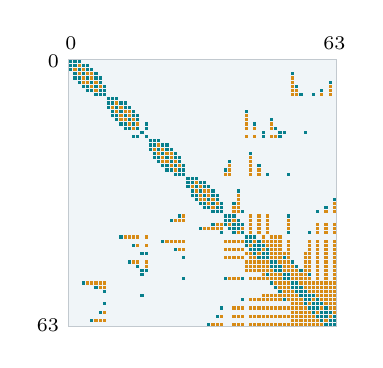
\begin{tikzpicture}[x=0.053125cm,y=0.053125cm]
\fill[Mist] (0,0) rectangle (64,-64);
\fill[Teal] (0.120,-0.120) rectangle (0.880,-0.880);
\fill[Teal] (1.120,-0.120) rectangle (1.880,-0.880);
\fill[Teal] (2.120,-0.120) rectangle (2.880,-0.880);
\fill[Teal] (0.120,-1.120) rectangle (0.880,-1.880);
\fill[Teal] (1.120,-1.120) rectangle (1.880,-1.880);
\fill[Amber] (2.120,-1.120) rectangle (2.880,-1.880);
\fill[Teal] (3.120,-1.120) rectangle (3.880,-1.880);
\fill[Teal] (4.120,-1.120) rectangle (4.880,-1.880);
\fill[Teal] (0.120,-2.120) rectangle (0.880,-2.880);
\fill[Amber] (1.120,-2.120) rectangle (1.880,-2.880);
\fill[Teal] (2.120,-2.120) rectangle (2.880,-2.880);
\fill[Amber] (3.120,-2.120) rectangle (3.880,-2.880);
\fill[Teal] (4.120,-2.120) rectangle (4.880,-2.880);
\fill[Teal] (5.120,-2.120) rectangle (5.880,-2.880);
\fill[Teal] (1.120,-3.120) rectangle (1.880,-3.880);
\fill[Amber] (2.120,-3.120) rectangle (2.880,-3.880);
\fill[Teal] (3.120,-3.120) rectangle (3.880,-3.880);
\fill[Amber] (4.120,-3.120) rectangle (4.880,-3.880);
\fill[Amber] (5.120,-3.120) rectangle (5.880,-3.880);
\fill[Teal] (6.120,-3.120) rectangle (6.880,-3.880);
\fill[Teal] (53.120,-3.120) rectangle (53.880,-3.880);
\fill[Teal] (1.120,-4.120) rectangle (1.880,-4.880);
\fill[Teal] (2.120,-4.120) rectangle (2.880,-4.880);
\fill[Amber] (3.120,-4.120) rectangle (3.880,-4.880);
\fill[Teal] (4.120,-4.120) rectangle (4.880,-4.880);
\fill[Amber] (5.120,-4.120) rectangle (5.880,-4.880);
\fill[Teal] (6.120,-4.120) rectangle (6.880,-4.880);
\fill[Teal] (7.120,-4.120) rectangle (7.880,-4.880);
\fill[Amber] (53.120,-4.120) rectangle (53.880,-4.880);
\fill[Teal] (2.120,-5.120) rectangle (2.880,-5.880);
\fill[Amber] (3.120,-5.120) rectangle (3.880,-5.880);
\fill[Amber] (4.120,-5.120) rectangle (4.880,-5.880);
\fill[Teal] (5.120,-5.120) rectangle (5.880,-5.880);
\fill[Amber] (6.120,-5.120) rectangle (6.880,-5.880);
\fill[Teal] (7.120,-5.120) rectangle (7.880,-5.880);
\fill[Amber] (53.120,-5.120) rectangle (53.880,-5.880);
\fill[Teal] (62.120,-5.120) rectangle (62.880,-5.880);
\fill[Teal] (3.120,-6.120) rectangle (3.880,-6.880);
\fill[Teal] (4.120,-6.120) rectangle (4.880,-6.880);
\fill[Amber] (5.120,-6.120) rectangle (5.880,-6.880);
\fill[Teal] (6.120,-6.120) rectangle (6.880,-6.880);
\fill[Amber] (7.120,-6.120) rectangle (7.880,-6.880);
\fill[Teal] (8.120,-6.120) rectangle (8.880,-6.880);
\fill[Amber] (53.120,-6.120) rectangle (53.880,-6.880);
\fill[Teal] (54.120,-6.120) rectangle (54.880,-6.880);
\fill[Amber] (62.120,-6.120) rectangle (62.880,-6.880);
\fill[Teal] (4.120,-7.120) rectangle (4.880,-7.880);
\fill[Teal] (5.120,-7.120) rectangle (5.880,-7.880);
\fill[Amber] (6.120,-7.120) rectangle (6.880,-7.880);
\fill[Teal] (7.120,-7.120) rectangle (7.880,-7.880);
\fill[Teal] (8.120,-7.120) rectangle (8.880,-7.880);
\fill[Amber] (53.120,-7.120) rectangle (53.880,-7.880);
\fill[Amber] (54.120,-7.120) rectangle (54.880,-7.880);
\fill[Teal] (60.120,-7.120) rectangle (60.880,-7.880);
\fill[Amber] (62.120,-7.120) rectangle (62.880,-7.880);
\fill[Teal] (6.120,-8.120) rectangle (6.880,-8.880);
\fill[Teal] (7.120,-8.120) rectangle (7.880,-8.880);
\fill[Teal] (8.120,-8.120) rectangle (8.880,-8.880);
\fill[Amber] (53.120,-8.120) rectangle (53.880,-8.880);
\fill[Amber] (54.120,-8.120) rectangle (54.880,-8.880);
\fill[Teal] (55.120,-8.120) rectangle (55.880,-8.880);
\fill[Teal] (58.120,-8.120) rectangle (58.880,-8.880);
\fill[Amber] (60.120,-8.120) rectangle (60.880,-8.880);
\fill[Amber] (62.120,-8.120) rectangle (62.880,-8.880);
\fill[Teal] (9.120,-9.120) rectangle (9.880,-9.880);
\fill[Teal] (10.120,-9.120) rectangle (10.880,-9.880);
\fill[Teal] (11.120,-9.120) rectangle (11.880,-9.880);
\fill[Teal] (9.120,-10.120) rectangle (9.880,-10.880);
\fill[Teal] (10.120,-10.120) rectangle (10.880,-10.880);
\fill[Amber] (11.120,-10.120) rectangle (11.880,-10.880);
\fill[Teal] (12.120,-10.120) rectangle (12.880,-10.880);
\fill[Teal] (13.120,-10.120) rectangle (13.880,-10.880);
\fill[Teal] (9.120,-11.120) rectangle (9.880,-11.880);
\fill[Amber] (10.120,-11.120) rectangle (10.880,-11.880);
\fill[Teal] (11.120,-11.120) rectangle (11.880,-11.880);
\fill[Amber] (12.120,-11.120) rectangle (12.880,-11.880);
\fill[Teal] (13.120,-11.120) rectangle (13.880,-11.880);
\fill[Teal] (14.120,-11.120) rectangle (14.880,-11.880);
\fill[Teal] (10.120,-12.120) rectangle (10.880,-12.880);
\fill[Amber] (11.120,-12.120) rectangle (11.880,-12.880);
\fill[Teal] (12.120,-12.120) rectangle (12.880,-12.880);
\fill[Amber] (13.120,-12.120) rectangle (13.880,-12.880);
\fill[Amber] (14.120,-12.120) rectangle (14.880,-12.880);
\fill[Teal] (15.120,-12.120) rectangle (15.880,-12.880);
\fill[Teal] (42.120,-12.120) rectangle (42.880,-12.880);
\fill[Teal] (10.120,-13.120) rectangle (10.880,-13.880);
\fill[Teal] (11.120,-13.120) rectangle (11.880,-13.880);
\fill[Amber] (12.120,-13.120) rectangle (12.880,-13.880);
\fill[Teal] (13.120,-13.120) rectangle (13.880,-13.880);
\fill[Amber] (14.120,-13.120) rectangle (14.880,-13.880);
\fill[Teal] (15.120,-13.120) rectangle (15.880,-13.880);
\fill[Teal] (16.120,-13.120) rectangle (16.880,-13.880);
\fill[Amber] (42.120,-13.120) rectangle (42.880,-13.880);
\fill[Teal] (11.120,-14.120) rectangle (11.880,-14.880);
\fill[Amber] (12.120,-14.120) rectangle (12.880,-14.880);
\fill[Amber] (13.120,-14.120) rectangle (13.880,-14.880);
\fill[Teal] (14.120,-14.120) rectangle (14.880,-14.880);
\fill[Amber] (15.120,-14.120) rectangle (15.880,-14.880);
\fill[Teal] (16.120,-14.120) rectangle (16.880,-14.880);
\fill[Amber] (42.120,-14.120) rectangle (42.880,-14.880);
\fill[Teal] (48.120,-14.120) rectangle (48.880,-14.880);
\fill[Teal] (12.120,-15.120) rectangle (12.880,-15.880);
\fill[Teal] (13.120,-15.120) rectangle (13.880,-15.880);
\fill[Amber] (14.120,-15.120) rectangle (14.880,-15.880);
\fill[Teal] (15.120,-15.120) rectangle (15.880,-15.880);
\fill[Amber] (16.120,-15.120) rectangle (16.880,-15.880);
\fill[Teal] (18.120,-15.120) rectangle (18.880,-15.880);
\fill[Amber] (42.120,-15.120) rectangle (42.880,-15.880);
\fill[Teal] (44.120,-15.120) rectangle (44.880,-15.880);
\fill[Amber] (48.120,-15.120) rectangle (48.880,-15.880);
\fill[Teal] (13.120,-16.120) rectangle (13.880,-16.880);
\fill[Teal] (14.120,-16.120) rectangle (14.880,-16.880);
\fill[Amber] (15.120,-16.120) rectangle (15.880,-16.880);
\fill[Teal] (16.120,-16.120) rectangle (16.880,-16.880);
\fill[Teal] (18.120,-16.120) rectangle (18.880,-16.880);
\fill[Amber] (42.120,-16.120) rectangle (42.880,-16.880);
\fill[Amber] (44.120,-16.120) rectangle (44.880,-16.880);
\fill[Amber] (48.120,-16.120) rectangle (48.880,-16.880);
\fill[Teal] (49.120,-16.120) rectangle (49.880,-16.880);
\fill[Teal] (17.120,-17.120) rectangle (17.880,-17.880);
\fill[Teal] (46.120,-17.120) rectangle (46.880,-17.880);
\fill[Teal] (50.120,-17.120) rectangle (50.880,-17.880);
\fill[Teal] (51.120,-17.120) rectangle (51.880,-17.880);
\fill[Teal] (56.120,-17.120) rectangle (56.880,-17.880);
\fill[Teal] (15.120,-18.120) rectangle (15.880,-18.880);
\fill[Teal] (16.120,-18.120) rectangle (16.880,-18.880);
\fill[Teal] (18.120,-18.120) rectangle (18.880,-18.880);
\fill[Amber] (42.120,-18.120) rectangle (42.880,-18.880);
\fill[Amber] (44.120,-18.120) rectangle (44.880,-18.880);
\fill[Teal] (46.120,-18.120) rectangle (46.880,-18.880);
\fill[Amber] (48.120,-18.120) rectangle (48.880,-18.880);
\fill[Amber] (49.120,-18.120) rectangle (49.880,-18.880);
\fill[Teal] (50.120,-18.120) rectangle (50.880,-18.880);
\fill[Teal] (19.120,-19.120) rectangle (19.880,-19.880);
\fill[Teal] (20.120,-19.120) rectangle (20.880,-19.880);
\fill[Teal] (21.120,-19.120) rectangle (21.880,-19.880);
\fill[Teal] (19.120,-20.120) rectangle (19.880,-20.880);
\fill[Teal] (20.120,-20.120) rectangle (20.880,-20.880);
\fill[Amber] (21.120,-20.120) rectangle (21.880,-20.880);
\fill[Teal] (22.120,-20.120) rectangle (22.880,-20.880);
\fill[Teal] (23.120,-20.120) rectangle (23.880,-20.880);
\fill[Teal] (19.120,-21.120) rectangle (19.880,-21.880);
\fill[Amber] (20.120,-21.120) rectangle (20.880,-21.880);
\fill[Teal] (21.120,-21.120) rectangle (21.880,-21.880);
\fill[Amber] (22.120,-21.120) rectangle (22.880,-21.880);
\fill[Teal] (23.120,-21.120) rectangle (23.880,-21.880);
\fill[Teal] (24.120,-21.120) rectangle (24.880,-21.880);
\fill[Teal] (20.120,-22.120) rectangle (20.880,-22.880);
\fill[Amber] (21.120,-22.120) rectangle (21.880,-22.880);
\fill[Teal] (22.120,-22.120) rectangle (22.880,-22.880);
\fill[Amber] (23.120,-22.120) rectangle (23.880,-22.880);
\fill[Amber] (24.120,-22.120) rectangle (24.880,-22.880);
\fill[Teal] (25.120,-22.120) rectangle (25.880,-22.880);
\fill[Teal] (43.120,-22.120) rectangle (43.880,-22.880);
\fill[Teal] (20.120,-23.120) rectangle (20.880,-23.880);
\fill[Teal] (21.120,-23.120) rectangle (21.880,-23.880);
\fill[Amber] (22.120,-23.120) rectangle (22.880,-23.880);
\fill[Teal] (23.120,-23.120) rectangle (23.880,-23.880);
\fill[Amber] (24.120,-23.120) rectangle (24.880,-23.880);
\fill[Teal] (25.120,-23.120) rectangle (25.880,-23.880);
\fill[Teal] (26.120,-23.120) rectangle (26.880,-23.880);
\fill[Amber] (43.120,-23.120) rectangle (43.880,-23.880);
\fill[Teal] (21.120,-24.120) rectangle (21.880,-24.880);
\fill[Amber] (22.120,-24.120) rectangle (22.880,-24.880);
\fill[Amber] (23.120,-24.120) rectangle (23.880,-24.880);
\fill[Teal] (24.120,-24.120) rectangle (24.880,-24.880);
\fill[Amber] (25.120,-24.120) rectangle (25.880,-24.880);
\fill[Teal] (26.120,-24.120) rectangle (26.880,-24.880);
\fill[Teal] (38.120,-24.120) rectangle (38.880,-24.880);
\fill[Amber] (43.120,-24.120) rectangle (43.880,-24.880);
\fill[Teal] (22.120,-25.120) rectangle (22.880,-25.880);
\fill[Teal] (23.120,-25.120) rectangle (23.880,-25.880);
\fill[Amber] (24.120,-25.120) rectangle (24.880,-25.880);
\fill[Teal] (25.120,-25.120) rectangle (25.880,-25.880);
\fill[Amber] (26.120,-25.120) rectangle (26.880,-25.880);
\fill[Teal] (27.120,-25.120) rectangle (27.880,-25.880);
\fill[Amber] (38.120,-25.120) rectangle (38.880,-25.880);
\fill[Amber] (43.120,-25.120) rectangle (43.880,-25.880);
\fill[Teal] (45.120,-25.120) rectangle (45.880,-25.880);
\fill[Teal] (23.120,-26.120) rectangle (23.880,-26.880);
\fill[Teal] (24.120,-26.120) rectangle (24.880,-26.880);
\fill[Amber] (25.120,-26.120) rectangle (25.880,-26.880);
\fill[Teal] (26.120,-26.120) rectangle (26.880,-26.880);
\fill[Teal] (27.120,-26.120) rectangle (27.880,-26.880);
\fill[Teal] (37.120,-26.120) rectangle (37.880,-26.880);
\fill[Amber] (38.120,-26.120) rectangle (38.880,-26.880);
\fill[Amber] (43.120,-26.120) rectangle (43.880,-26.880);
\fill[Amber] (45.120,-26.120) rectangle (45.880,-26.880);
\fill[Teal] (25.120,-27.120) rectangle (25.880,-27.880);
\fill[Teal] (26.120,-27.120) rectangle (26.880,-27.880);
\fill[Teal] (27.120,-27.120) rectangle (27.880,-27.880);
\fill[Amber] (37.120,-27.120) rectangle (37.880,-27.880);
\fill[Amber] (38.120,-27.120) rectangle (38.880,-27.880);
\fill[Amber] (43.120,-27.120) rectangle (43.880,-27.880);
\fill[Amber] (45.120,-27.120) rectangle (45.880,-27.880);
\fill[Teal] (47.120,-27.120) rectangle (47.880,-27.880);
\fill[Teal] (52.120,-27.120) rectangle (52.880,-27.880);
\fill[Teal] (28.120,-28.120) rectangle (28.880,-28.880);
\fill[Teal] (29.120,-28.120) rectangle (29.880,-28.880);
\fill[Teal] (30.120,-28.120) rectangle (30.880,-28.880);
\fill[Teal] (28.120,-29.120) rectangle (28.880,-29.880);
\fill[Teal] (29.120,-29.120) rectangle (29.880,-29.880);
\fill[Amber] (30.120,-29.120) rectangle (30.880,-29.880);
\fill[Teal] (31.120,-29.120) rectangle (31.880,-29.880);
\fill[Teal] (32.120,-29.120) rectangle (32.880,-29.880);
\fill[Teal] (28.120,-30.120) rectangle (28.880,-30.880);
\fill[Amber] (29.120,-30.120) rectangle (29.880,-30.880);
\fill[Teal] (30.120,-30.120) rectangle (30.880,-30.880);
\fill[Amber] (31.120,-30.120) rectangle (31.880,-30.880);
\fill[Teal] (32.120,-30.120) rectangle (32.880,-30.880);
\fill[Teal] (33.120,-30.120) rectangle (33.880,-30.880);
\fill[Teal] (29.120,-31.120) rectangle (29.880,-31.880);
\fill[Amber] (30.120,-31.120) rectangle (30.880,-31.880);
\fill[Teal] (31.120,-31.120) rectangle (31.880,-31.880);
\fill[Amber] (32.120,-31.120) rectangle (32.880,-31.880);
\fill[Amber] (33.120,-31.120) rectangle (33.880,-31.880);
\fill[Teal] (34.120,-31.120) rectangle (34.880,-31.880);
\fill[Teal] (40.120,-31.120) rectangle (40.880,-31.880);
\fill[Teal] (29.120,-32.120) rectangle (29.880,-32.880);
\fill[Teal] (30.120,-32.120) rectangle (30.880,-32.880);
\fill[Amber] (31.120,-32.120) rectangle (31.880,-32.880);
\fill[Teal] (32.120,-32.120) rectangle (32.880,-32.880);
\fill[Amber] (33.120,-32.120) rectangle (33.880,-32.880);
\fill[Teal] (34.120,-32.120) rectangle (34.880,-32.880);
\fill[Teal] (35.120,-32.120) rectangle (35.880,-32.880);
\fill[Amber] (40.120,-32.120) rectangle (40.880,-32.880);
\fill[Teal] (30.120,-33.120) rectangle (30.880,-33.880);
\fill[Amber] (31.120,-33.120) rectangle (31.880,-33.880);
\fill[Amber] (32.120,-33.120) rectangle (32.880,-33.880);
\fill[Teal] (33.120,-33.120) rectangle (33.880,-33.880);
\fill[Amber] (34.120,-33.120) rectangle (34.880,-33.880);
\fill[Teal] (35.120,-33.120) rectangle (35.880,-33.880);
\fill[Amber] (40.120,-33.120) rectangle (40.880,-33.880);
\fill[Teal] (63.120,-33.120) rectangle (63.880,-33.880);
\fill[Teal] (31.120,-34.120) rectangle (31.880,-34.880);
\fill[Teal] (32.120,-34.120) rectangle (32.880,-34.880);
\fill[Amber] (33.120,-34.120) rectangle (33.880,-34.880);
\fill[Teal] (34.120,-34.120) rectangle (34.880,-34.880);
\fill[Amber] (35.120,-34.120) rectangle (35.880,-34.880);
\fill[Teal] (36.120,-34.120) rectangle (36.880,-34.880);
\fill[Teal] (39.120,-34.120) rectangle (39.880,-34.880);
\fill[Amber] (40.120,-34.120) rectangle (40.880,-34.880);
\fill[Amber] (63.120,-34.120) rectangle (63.880,-34.880);
\fill[Teal] (32.120,-35.120) rectangle (32.880,-35.880);
\fill[Teal] (33.120,-35.120) rectangle (33.880,-35.880);
\fill[Amber] (34.120,-35.120) rectangle (34.880,-35.880);
\fill[Teal] (35.120,-35.120) rectangle (35.880,-35.880);
\fill[Teal] (36.120,-35.120) rectangle (36.880,-35.880);
\fill[Amber] (39.120,-35.120) rectangle (39.880,-35.880);
\fill[Amber] (40.120,-35.120) rectangle (40.880,-35.880);
\fill[Teal] (61.120,-35.120) rectangle (61.880,-35.880);
\fill[Amber] (63.120,-35.120) rectangle (63.880,-35.880);
\fill[Teal] (34.120,-36.120) rectangle (34.880,-36.880);
\fill[Teal] (35.120,-36.120) rectangle (35.880,-36.880);
\fill[Teal] (36.120,-36.120) rectangle (36.880,-36.880);
\fill[Amber] (39.120,-36.120) rectangle (39.880,-36.880);
\fill[Amber] (40.120,-36.120) rectangle (40.880,-36.880);
\fill[Teal] (41.120,-36.120) rectangle (41.880,-36.880);
\fill[Teal] (59.120,-36.120) rectangle (59.880,-36.880);
\fill[Amber] (61.120,-36.120) rectangle (61.880,-36.880);
\fill[Amber] (63.120,-36.120) rectangle (63.880,-36.880);
\fill[Teal] (26.120,-37.120) rectangle (26.880,-37.880);
\fill[Amber] (27.120,-37.120) rectangle (27.880,-37.880);
\fill[Teal] (37.120,-37.120) rectangle (37.880,-37.880);
\fill[Teal] (38.120,-37.120) rectangle (38.880,-37.880);
\fill[Teal] (39.120,-37.120) rectangle (39.880,-37.880);
\fill[Amber] (43.120,-37.120) rectangle (43.880,-37.880);
\fill[Amber] (45.120,-37.120) rectangle (45.880,-37.880);
\fill[Amber] (47.120,-37.120) rectangle (47.880,-37.880);
\fill[Teal] (52.120,-37.120) rectangle (52.880,-37.880);
\fill[Teal] (24.120,-38.120) rectangle (24.880,-38.880);
\fill[Amber] (25.120,-38.120) rectangle (25.880,-38.880);
\fill[Amber] (26.120,-38.120) rectangle (26.880,-38.880);
\fill[Amber] (27.120,-38.120) rectangle (27.880,-38.880);
\fill[Teal] (37.120,-38.120) rectangle (37.880,-38.880);
\fill[Teal] (38.120,-38.120) rectangle (38.880,-38.880);
\fill[Amber] (39.120,-38.120) rectangle (39.880,-38.880);
\fill[Teal] (40.120,-38.120) rectangle (40.880,-38.880);
\fill[Amber] (43.120,-38.120) rectangle (43.880,-38.880);
\fill[Amber] (45.120,-38.120) rectangle (45.880,-38.880);
\fill[Amber] (47.120,-38.120) rectangle (47.880,-38.880);
\fill[Amber] (52.120,-38.120) rectangle (52.880,-38.880);
\fill[Teal] (34.120,-39.120) rectangle (34.880,-39.880);
\fill[Amber] (35.120,-39.120) rectangle (35.880,-39.880);
\fill[Amber] (36.120,-39.120) rectangle (36.880,-39.880);
\fill[Teal] (37.120,-39.120) rectangle (37.880,-39.880);
\fill[Amber] (38.120,-39.120) rectangle (38.880,-39.880);
\fill[Teal] (39.120,-39.120) rectangle (39.880,-39.880);
\fill[Teal] (40.120,-39.120) rectangle (40.880,-39.880);
\fill[Teal] (41.120,-39.120) rectangle (41.880,-39.880);
\fill[Amber] (43.120,-39.120) rectangle (43.880,-39.880);
\fill[Amber] (45.120,-39.120) rectangle (45.880,-39.880);
\fill[Amber] (47.120,-39.120) rectangle (47.880,-39.880);
\fill[Amber] (52.120,-39.120) rectangle (52.880,-39.880);
\fill[Amber] (59.120,-39.120) rectangle (59.880,-39.880);
\fill[Amber] (61.120,-39.120) rectangle (61.880,-39.880);
\fill[Amber] (63.120,-39.120) rectangle (63.880,-39.880);
\fill[Teal] (31.120,-40.120) rectangle (31.880,-40.880);
\fill[Amber] (32.120,-40.120) rectangle (32.880,-40.880);
\fill[Amber] (33.120,-40.120) rectangle (33.880,-40.880);
\fill[Amber] (34.120,-40.120) rectangle (34.880,-40.880);
\fill[Amber] (35.120,-40.120) rectangle (35.880,-40.880);
\fill[Amber] (36.120,-40.120) rectangle (36.880,-40.880);
\fill[Teal] (38.120,-40.120) rectangle (38.880,-40.880);
\fill[Teal] (39.120,-40.120) rectangle (39.880,-40.880);
\fill[Teal] (40.120,-40.120) rectangle (40.880,-40.880);
\fill[Amber] (41.120,-40.120) rectangle (41.880,-40.880);
\fill[Amber] (43.120,-40.120) rectangle (43.880,-40.880);
\fill[Amber] (45.120,-40.120) rectangle (45.880,-40.880);
\fill[Amber] (47.120,-40.120) rectangle (47.880,-40.880);
\fill[Amber] (52.120,-40.120) rectangle (52.880,-40.880);
\fill[Amber] (59.120,-40.120) rectangle (59.880,-40.880);
\fill[Amber] (61.120,-40.120) rectangle (61.880,-40.880);
\fill[Amber] (63.120,-40.120) rectangle (63.880,-40.880);
\fill[Teal] (36.120,-41.120) rectangle (36.880,-41.880);
\fill[Teal] (39.120,-41.120) rectangle (39.880,-41.880);
\fill[Amber] (40.120,-41.120) rectangle (40.880,-41.880);
\fill[Teal] (41.120,-41.120) rectangle (41.880,-41.880);
\fill[Amber] (43.120,-41.120) rectangle (43.880,-41.880);
\fill[Amber] (45.120,-41.120) rectangle (45.880,-41.880);
\fill[Amber] (47.120,-41.120) rectangle (47.880,-41.880);
\fill[Teal] (52.120,-41.120) rectangle (52.880,-41.880);
\fill[Teal] (57.120,-41.120) rectangle (57.880,-41.880);
\fill[Amber] (59.120,-41.120) rectangle (59.880,-41.880);
\fill[Amber] (61.120,-41.120) rectangle (61.880,-41.880);
\fill[Amber] (63.120,-41.120) rectangle (63.880,-41.880);
\fill[Teal] (12.120,-42.120) rectangle (12.880,-42.880);
\fill[Amber] (13.120,-42.120) rectangle (13.880,-42.880);
\fill[Amber] (14.120,-42.120) rectangle (14.880,-42.880);
\fill[Amber] (15.120,-42.120) rectangle (15.880,-42.880);
\fill[Amber] (16.120,-42.120) rectangle (16.880,-42.880);
\fill[Amber] (18.120,-42.120) rectangle (18.880,-42.880);
\fill[Teal] (42.120,-42.120) rectangle (42.880,-42.880);
\fill[Teal] (43.120,-42.120) rectangle (43.880,-42.880);
\fill[Teal] (44.120,-42.120) rectangle (44.880,-42.880);
\fill[Amber] (46.120,-42.120) rectangle (46.880,-42.880);
\fill[Amber] (48.120,-42.120) rectangle (48.880,-42.880);
\fill[Amber] (49.120,-42.120) rectangle (49.880,-42.880);
\fill[Amber] (50.120,-42.120) rectangle (50.880,-42.880);
\fill[Teal] (22.120,-43.120) rectangle (22.880,-43.880);
\fill[Amber] (23.120,-43.120) rectangle (23.880,-43.880);
\fill[Amber] (24.120,-43.120) rectangle (24.880,-43.880);
\fill[Amber] (25.120,-43.120) rectangle (25.880,-43.880);
\fill[Amber] (26.120,-43.120) rectangle (26.880,-43.880);
\fill[Amber] (27.120,-43.120) rectangle (27.880,-43.880);
\fill[Amber] (37.120,-43.120) rectangle (37.880,-43.880);
\fill[Amber] (38.120,-43.120) rectangle (38.880,-43.880);
\fill[Amber] (39.120,-43.120) rectangle (39.880,-43.880);
\fill[Amber] (40.120,-43.120) rectangle (40.880,-43.880);
\fill[Amber] (41.120,-43.120) rectangle (41.880,-43.880);
\fill[Teal] (42.120,-43.120) rectangle (42.880,-43.880);
\fill[Teal] (43.120,-43.120) rectangle (43.880,-43.880);
\fill[Amber] (44.120,-43.120) rectangle (44.880,-43.880);
\fill[Teal] (45.120,-43.120) rectangle (45.880,-43.880);
\fill[Amber] (46.120,-43.120) rectangle (46.880,-43.880);
\fill[Amber] (47.120,-43.120) rectangle (47.880,-43.880);
\fill[Amber] (48.120,-43.120) rectangle (48.880,-43.880);
\fill[Amber] (49.120,-43.120) rectangle (49.880,-43.880);
\fill[Amber] (50.120,-43.120) rectangle (50.880,-43.880);
\fill[Amber] (52.120,-43.120) rectangle (52.880,-43.880);
\fill[Amber] (57.120,-43.120) rectangle (57.880,-43.880);
\fill[Amber] (59.120,-43.120) rectangle (59.880,-43.880);
\fill[Amber] (61.120,-43.120) rectangle (61.880,-43.880);
\fill[Amber] (63.120,-43.120) rectangle (63.880,-43.880);
\fill[Teal] (15.120,-44.120) rectangle (15.880,-44.880);
\fill[Amber] (16.120,-44.120) rectangle (16.880,-44.880);
\fill[Amber] (18.120,-44.120) rectangle (18.880,-44.880);
\fill[Teal] (42.120,-44.120) rectangle (42.880,-44.880);
\fill[Amber] (43.120,-44.120) rectangle (43.880,-44.880);
\fill[Teal] (44.120,-44.120) rectangle (44.880,-44.880);
\fill[Teal] (45.120,-44.120) rectangle (45.880,-44.880);
\fill[Teal] (46.120,-44.120) rectangle (46.880,-44.880);
\fill[Amber] (47.120,-44.120) rectangle (47.880,-44.880);
\fill[Amber] (48.120,-44.120) rectangle (48.880,-44.880);
\fill[Amber] (49.120,-44.120) rectangle (49.880,-44.880);
\fill[Amber] (50.120,-44.120) rectangle (50.880,-44.880);
\fill[Amber] (52.120,-44.120) rectangle (52.880,-44.880);
\fill[Amber] (57.120,-44.120) rectangle (57.880,-44.880);
\fill[Amber] (59.120,-44.120) rectangle (59.880,-44.880);
\fill[Amber] (61.120,-44.120) rectangle (61.880,-44.880);
\fill[Amber] (63.120,-44.120) rectangle (63.880,-44.880);
\fill[Teal] (25.120,-45.120) rectangle (25.880,-45.880);
\fill[Amber] (26.120,-45.120) rectangle (26.880,-45.880);
\fill[Amber] (27.120,-45.120) rectangle (27.880,-45.880);
\fill[Amber] (37.120,-45.120) rectangle (37.880,-45.880);
\fill[Amber] (38.120,-45.120) rectangle (38.880,-45.880);
\fill[Amber] (39.120,-45.120) rectangle (39.880,-45.880);
\fill[Amber] (40.120,-45.120) rectangle (40.880,-45.880);
\fill[Amber] (41.120,-45.120) rectangle (41.880,-45.880);
\fill[Teal] (43.120,-45.120) rectangle (43.880,-45.880);
\fill[Teal] (44.120,-45.120) rectangle (44.880,-45.880);
\fill[Teal] (45.120,-45.120) rectangle (45.880,-45.880);
\fill[Amber] (46.120,-45.120) rectangle (46.880,-45.880);
\fill[Teal] (47.120,-45.120) rectangle (47.880,-45.880);
\fill[Amber] (48.120,-45.120) rectangle (48.880,-45.880);
\fill[Amber] (49.120,-45.120) rectangle (49.880,-45.880);
\fill[Amber] (50.120,-45.120) rectangle (50.880,-45.880);
\fill[Amber] (52.120,-45.120) rectangle (52.880,-45.880);
\fill[Amber] (57.120,-45.120) rectangle (57.880,-45.880);
\fill[Amber] (59.120,-45.120) rectangle (59.880,-45.880);
\fill[Amber] (61.120,-45.120) rectangle (61.880,-45.880);
\fill[Amber] (63.120,-45.120) rectangle (63.880,-45.880);
\fill[Teal] (17.120,-46.120) rectangle (17.880,-46.880);
\fill[Teal] (18.120,-46.120) rectangle (18.880,-46.880);
\fill[Amber] (42.120,-46.120) rectangle (42.880,-46.880);
\fill[Amber] (43.120,-46.120) rectangle (43.880,-46.880);
\fill[Teal] (44.120,-46.120) rectangle (44.880,-46.880);
\fill[Amber] (45.120,-46.120) rectangle (45.880,-46.880);
\fill[Teal] (46.120,-46.120) rectangle (46.880,-46.880);
\fill[Teal] (47.120,-46.120) rectangle (47.880,-46.880);
\fill[Amber] (48.120,-46.120) rectangle (48.880,-46.880);
\fill[Amber] (49.120,-46.120) rectangle (49.880,-46.880);
\fill[Amber] (50.120,-46.120) rectangle (50.880,-46.880);
\fill[Amber] (51.120,-46.120) rectangle (51.880,-46.880);
\fill[Amber] (52.120,-46.120) rectangle (52.880,-46.880);
\fill[Amber] (56.120,-46.120) rectangle (56.880,-46.880);
\fill[Amber] (57.120,-46.120) rectangle (57.880,-46.880);
\fill[Amber] (59.120,-46.120) rectangle (59.880,-46.880);
\fill[Amber] (61.120,-46.120) rectangle (61.880,-46.880);
\fill[Amber] (63.120,-46.120) rectangle (63.880,-46.880);
\fill[Teal] (27.120,-47.120) rectangle (27.880,-47.880);
\fill[Amber] (37.120,-47.120) rectangle (37.880,-47.880);
\fill[Amber] (38.120,-47.120) rectangle (38.880,-47.880);
\fill[Amber] (39.120,-47.120) rectangle (39.880,-47.880);
\fill[Amber] (40.120,-47.120) rectangle (40.880,-47.880);
\fill[Amber] (41.120,-47.120) rectangle (41.880,-47.880);
\fill[Amber] (43.120,-47.120) rectangle (43.880,-47.880);
\fill[Amber] (44.120,-47.120) rectangle (44.880,-47.880);
\fill[Teal] (45.120,-47.120) rectangle (45.880,-47.880);
\fill[Teal] (46.120,-47.120) rectangle (46.880,-47.880);
\fill[Teal] (47.120,-47.120) rectangle (47.880,-47.880);
\fill[Amber] (48.120,-47.120) rectangle (48.880,-47.880);
\fill[Amber] (49.120,-47.120) rectangle (49.880,-47.880);
\fill[Amber] (50.120,-47.120) rectangle (50.880,-47.880);
\fill[Teal] (51.120,-47.120) rectangle (51.880,-47.880);
\fill[Amber] (52.120,-47.120) rectangle (52.880,-47.880);
\fill[Amber] (56.120,-47.120) rectangle (56.880,-47.880);
\fill[Amber] (57.120,-47.120) rectangle (57.880,-47.880);
\fill[Amber] (59.120,-47.120) rectangle (59.880,-47.880);
\fill[Amber] (61.120,-47.120) rectangle (61.880,-47.880);
\fill[Amber] (63.120,-47.120) rectangle (63.880,-47.880);
\fill[Teal] (14.120,-48.120) rectangle (14.880,-48.880);
\fill[Amber] (15.120,-48.120) rectangle (15.880,-48.880);
\fill[Amber] (16.120,-48.120) rectangle (16.880,-48.880);
\fill[Amber] (18.120,-48.120) rectangle (18.880,-48.880);
\fill[Amber] (42.120,-48.120) rectangle (42.880,-48.880);
\fill[Amber] (43.120,-48.120) rectangle (43.880,-48.880);
\fill[Amber] (44.120,-48.120) rectangle (44.880,-48.880);
\fill[Amber] (45.120,-48.120) rectangle (45.880,-48.880);
\fill[Amber] (46.120,-48.120) rectangle (46.880,-48.880);
\fill[Amber] (47.120,-48.120) rectangle (47.880,-48.880);
\fill[Teal] (48.120,-48.120) rectangle (48.880,-48.880);
\fill[Teal] (49.120,-48.120) rectangle (49.880,-48.880);
\fill[Amber] (50.120,-48.120) rectangle (50.880,-48.880);
\fill[Amber] (51.120,-48.120) rectangle (51.880,-48.880);
\fill[Amber] (52.120,-48.120) rectangle (52.880,-48.880);
\fill[Teal] (53.120,-48.120) rectangle (53.880,-48.880);
\fill[Amber] (56.120,-48.120) rectangle (56.880,-48.880);
\fill[Amber] (57.120,-48.120) rectangle (57.880,-48.880);
\fill[Amber] (59.120,-48.120) rectangle (59.880,-48.880);
\fill[Amber] (61.120,-48.120) rectangle (61.880,-48.880);
\fill[Amber] (63.120,-48.120) rectangle (63.880,-48.880);
\fill[Teal] (16.120,-49.120) rectangle (16.880,-49.880);
\fill[Amber] (18.120,-49.120) rectangle (18.880,-49.880);
\fill[Amber] (42.120,-49.120) rectangle (42.880,-49.880);
\fill[Amber] (43.120,-49.120) rectangle (43.880,-49.880);
\fill[Amber] (44.120,-49.120) rectangle (44.880,-49.880);
\fill[Amber] (45.120,-49.120) rectangle (45.880,-49.880);
\fill[Amber] (46.120,-49.120) rectangle (46.880,-49.880);
\fill[Amber] (47.120,-49.120) rectangle (47.880,-49.880);
\fill[Teal] (48.120,-49.120) rectangle (48.880,-49.880);
\fill[Teal] (49.120,-49.120) rectangle (49.880,-49.880);
\fill[Teal] (50.120,-49.120) rectangle (50.880,-49.880);
\fill[Amber] (51.120,-49.120) rectangle (51.880,-49.880);
\fill[Amber] (52.120,-49.120) rectangle (52.880,-49.880);
\fill[Amber] (53.120,-49.120) rectangle (53.880,-49.880);
\fill[Teal] (54.120,-49.120) rectangle (54.880,-49.880);
\fill[Amber] (56.120,-49.120) rectangle (56.880,-49.880);
\fill[Amber] (57.120,-49.120) rectangle (57.880,-49.880);
\fill[Amber] (59.120,-49.120) rectangle (59.880,-49.880);
\fill[Amber] (61.120,-49.120) rectangle (61.880,-49.880);
\fill[Amber] (63.120,-49.120) rectangle (63.880,-49.880);
\fill[Teal] (17.120,-50.120) rectangle (17.880,-50.880);
\fill[Teal] (18.120,-50.120) rectangle (18.880,-50.880);
\fill[Amber] (42.120,-50.120) rectangle (42.880,-50.880);
\fill[Amber] (43.120,-50.120) rectangle (43.880,-50.880);
\fill[Amber] (44.120,-50.120) rectangle (44.880,-50.880);
\fill[Amber] (45.120,-50.120) rectangle (45.880,-50.880);
\fill[Amber] (46.120,-50.120) rectangle (46.880,-50.880);
\fill[Amber] (47.120,-50.120) rectangle (47.880,-50.880);
\fill[Amber] (48.120,-50.120) rectangle (48.880,-50.880);
\fill[Teal] (49.120,-50.120) rectangle (49.880,-50.880);
\fill[Teal] (50.120,-50.120) rectangle (50.880,-50.880);
\fill[Amber] (51.120,-50.120) rectangle (51.880,-50.880);
\fill[Amber] (52.120,-50.120) rectangle (52.880,-50.880);
\fill[Amber] (53.120,-50.120) rectangle (53.880,-50.880);
\fill[Amber] (54.120,-50.120) rectangle (54.880,-50.880);
\fill[Teal] (55.120,-50.120) rectangle (55.880,-50.880);
\fill[Amber] (56.120,-50.120) rectangle (56.880,-50.880);
\fill[Amber] (57.120,-50.120) rectangle (57.880,-50.880);
\fill[Amber] (59.120,-50.120) rectangle (59.880,-50.880);
\fill[Amber] (61.120,-50.120) rectangle (61.880,-50.880);
\fill[Amber] (63.120,-50.120) rectangle (63.880,-50.880);
\fill[Teal] (17.120,-51.120) rectangle (17.880,-51.880);
\fill[Amber] (46.120,-51.120) rectangle (46.880,-51.880);
\fill[Teal] (47.120,-51.120) rectangle (47.880,-51.880);
\fill[Amber] (48.120,-51.120) rectangle (48.880,-51.880);
\fill[Amber] (49.120,-51.120) rectangle (49.880,-51.880);
\fill[Amber] (50.120,-51.120) rectangle (50.880,-51.880);
\fill[Teal] (51.120,-51.120) rectangle (51.880,-51.880);
\fill[Teal] (52.120,-51.120) rectangle (52.880,-51.880);
\fill[Amber] (53.120,-51.120) rectangle (53.880,-51.880);
\fill[Amber] (54.120,-51.120) rectangle (54.880,-51.880);
\fill[Amber] (55.120,-51.120) rectangle (55.880,-51.880);
\fill[Amber] (56.120,-51.120) rectangle (56.880,-51.880);
\fill[Teal] (57.120,-51.120) rectangle (57.880,-51.880);
\fill[Amber] (59.120,-51.120) rectangle (59.880,-51.880);
\fill[Amber] (61.120,-51.120) rectangle (61.880,-51.880);
\fill[Amber] (63.120,-51.120) rectangle (63.880,-51.880);
\fill[Teal] (27.120,-52.120) rectangle (27.880,-52.880);
\fill[Teal] (37.120,-52.120) rectangle (37.880,-52.880);
\fill[Amber] (38.120,-52.120) rectangle (38.880,-52.880);
\fill[Amber] (39.120,-52.120) rectangle (39.880,-52.880);
\fill[Amber] (40.120,-52.120) rectangle (40.880,-52.880);
\fill[Teal] (41.120,-52.120) rectangle (41.880,-52.880);
\fill[Amber] (43.120,-52.120) rectangle (43.880,-52.880);
\fill[Amber] (44.120,-52.120) rectangle (44.880,-52.880);
\fill[Amber] (45.120,-52.120) rectangle (45.880,-52.880);
\fill[Amber] (46.120,-52.120) rectangle (46.880,-52.880);
\fill[Amber] (47.120,-52.120) rectangle (47.880,-52.880);
\fill[Amber] (48.120,-52.120) rectangle (48.880,-52.880);
\fill[Amber] (49.120,-52.120) rectangle (49.880,-52.880);
\fill[Amber] (50.120,-52.120) rectangle (50.880,-52.880);
\fill[Teal] (51.120,-52.120) rectangle (51.880,-52.880);
\fill[Teal] (52.120,-52.120) rectangle (52.880,-52.880);
\fill[Amber] (53.120,-52.120) rectangle (53.880,-52.880);
\fill[Amber] (54.120,-52.120) rectangle (54.880,-52.880);
\fill[Amber] (55.120,-52.120) rectangle (55.880,-52.880);
\fill[Amber] (56.120,-52.120) rectangle (56.880,-52.880);
\fill[Amber] (57.120,-52.120) rectangle (57.880,-52.880);
\fill[Amber] (59.120,-52.120) rectangle (59.880,-52.880);
\fill[Amber] (61.120,-52.120) rectangle (61.880,-52.880);
\fill[Amber] (63.120,-52.120) rectangle (63.880,-52.880);
\fill[Teal] (3.120,-53.120) rectangle (3.880,-53.880);
\fill[Amber] (4.120,-53.120) rectangle (4.880,-53.880);
\fill[Amber] (5.120,-53.120) rectangle (5.880,-53.880);
\fill[Amber] (6.120,-53.120) rectangle (6.880,-53.880);
\fill[Amber] (7.120,-53.120) rectangle (7.880,-53.880);
\fill[Amber] (8.120,-53.120) rectangle (8.880,-53.880);
\fill[Teal] (48.120,-53.120) rectangle (48.880,-53.880);
\fill[Amber] (49.120,-53.120) rectangle (49.880,-53.880);
\fill[Amber] (50.120,-53.120) rectangle (50.880,-53.880);
\fill[Amber] (51.120,-53.120) rectangle (51.880,-53.880);
\fill[Amber] (52.120,-53.120) rectangle (52.880,-53.880);
\fill[Teal] (53.120,-53.120) rectangle (53.880,-53.880);
\fill[Teal] (54.120,-53.120) rectangle (54.880,-53.880);
\fill[Amber] (55.120,-53.120) rectangle (55.880,-53.880);
\fill[Amber] (56.120,-53.120) rectangle (56.880,-53.880);
\fill[Amber] (57.120,-53.120) rectangle (57.880,-53.880);
\fill[Amber] (58.120,-53.120) rectangle (58.880,-53.880);
\fill[Amber] (59.120,-53.120) rectangle (59.880,-53.880);
\fill[Amber] (60.120,-53.120) rectangle (60.880,-53.880);
\fill[Amber] (61.120,-53.120) rectangle (61.880,-53.880);
\fill[Amber] (62.120,-53.120) rectangle (62.880,-53.880);
\fill[Amber] (63.120,-53.120) rectangle (63.880,-53.880);
\fill[Teal] (6.120,-54.120) rectangle (6.880,-54.880);
\fill[Amber] (7.120,-54.120) rectangle (7.880,-54.880);
\fill[Amber] (8.120,-54.120) rectangle (8.880,-54.880);
\fill[Teal] (49.120,-54.120) rectangle (49.880,-54.880);
\fill[Amber] (50.120,-54.120) rectangle (50.880,-54.880);
\fill[Amber] (51.120,-54.120) rectangle (51.880,-54.880);
\fill[Amber] (52.120,-54.120) rectangle (52.880,-54.880);
\fill[Teal] (53.120,-54.120) rectangle (53.880,-54.880);
\fill[Teal] (54.120,-54.120) rectangle (54.880,-54.880);
\fill[Teal] (55.120,-54.120) rectangle (55.880,-54.880);
\fill[Amber] (56.120,-54.120) rectangle (56.880,-54.880);
\fill[Amber] (57.120,-54.120) rectangle (57.880,-54.880);
\fill[Amber] (58.120,-54.120) rectangle (58.880,-54.880);
\fill[Amber] (59.120,-54.120) rectangle (59.880,-54.880);
\fill[Amber] (60.120,-54.120) rectangle (60.880,-54.880);
\fill[Amber] (61.120,-54.120) rectangle (61.880,-54.880);
\fill[Amber] (62.120,-54.120) rectangle (62.880,-54.880);
\fill[Amber] (63.120,-54.120) rectangle (63.880,-54.880);
\fill[Teal] (8.120,-55.120) rectangle (8.880,-55.880);
\fill[Teal] (50.120,-55.120) rectangle (50.880,-55.880);
\fill[Amber] (51.120,-55.120) rectangle (51.880,-55.880);
\fill[Amber] (52.120,-55.120) rectangle (52.880,-55.880);
\fill[Amber] (53.120,-55.120) rectangle (53.880,-55.880);
\fill[Teal] (54.120,-55.120) rectangle (54.880,-55.880);
\fill[Teal] (55.120,-55.120) rectangle (55.880,-55.880);
\fill[Teal] (56.120,-55.120) rectangle (56.880,-55.880);
\fill[Amber] (57.120,-55.120) rectangle (57.880,-55.880);
\fill[Amber] (58.120,-55.120) rectangle (58.880,-55.880);
\fill[Amber] (59.120,-55.120) rectangle (59.880,-55.880);
\fill[Amber] (60.120,-55.120) rectangle (60.880,-55.880);
\fill[Amber] (61.120,-55.120) rectangle (61.880,-55.880);
\fill[Amber] (62.120,-55.120) rectangle (62.880,-55.880);
\fill[Amber] (63.120,-55.120) rectangle (63.880,-55.880);
\fill[Teal] (17.120,-56.120) rectangle (17.880,-56.880);
\fill[Amber] (46.120,-56.120) rectangle (46.880,-56.880);
\fill[Amber] (47.120,-56.120) rectangle (47.880,-56.880);
\fill[Amber] (48.120,-56.120) rectangle (48.880,-56.880);
\fill[Amber] (49.120,-56.120) rectangle (49.880,-56.880);
\fill[Amber] (50.120,-56.120) rectangle (50.880,-56.880);
\fill[Amber] (51.120,-56.120) rectangle (51.880,-56.880);
\fill[Amber] (52.120,-56.120) rectangle (52.880,-56.880);
\fill[Amber] (53.120,-56.120) rectangle (53.880,-56.880);
\fill[Amber] (54.120,-56.120) rectangle (54.880,-56.880);
\fill[Teal] (55.120,-56.120) rectangle (55.880,-56.880);
\fill[Teal] (56.120,-56.120) rectangle (56.880,-56.880);
\fill[Teal] (57.120,-56.120) rectangle (57.880,-56.880);
\fill[Teal] (58.120,-56.120) rectangle (58.880,-56.880);
\fill[Amber] (59.120,-56.120) rectangle (59.880,-56.880);
\fill[Amber] (60.120,-56.120) rectangle (60.880,-56.880);
\fill[Amber] (61.120,-56.120) rectangle (61.880,-56.880);
\fill[Amber] (62.120,-56.120) rectangle (62.880,-56.880);
\fill[Amber] (63.120,-56.120) rectangle (63.880,-56.880);
\fill[Teal] (41.120,-57.120) rectangle (41.880,-57.880);
\fill[Amber] (43.120,-57.120) rectangle (43.880,-57.880);
\fill[Amber] (44.120,-57.120) rectangle (44.880,-57.880);
\fill[Amber] (45.120,-57.120) rectangle (45.880,-57.880);
\fill[Amber] (46.120,-57.120) rectangle (46.880,-57.880);
\fill[Amber] (47.120,-57.120) rectangle (47.880,-57.880);
\fill[Amber] (48.120,-57.120) rectangle (48.880,-57.880);
\fill[Amber] (49.120,-57.120) rectangle (49.880,-57.880);
\fill[Amber] (50.120,-57.120) rectangle (50.880,-57.880);
\fill[Teal] (51.120,-57.120) rectangle (51.880,-57.880);
\fill[Amber] (52.120,-57.120) rectangle (52.880,-57.880);
\fill[Amber] (53.120,-57.120) rectangle (53.880,-57.880);
\fill[Amber] (54.120,-57.120) rectangle (54.880,-57.880);
\fill[Amber] (55.120,-57.120) rectangle (55.880,-57.880);
\fill[Teal] (56.120,-57.120) rectangle (56.880,-57.880);
\fill[Teal] (57.120,-57.120) rectangle (57.880,-57.880);
\fill[Amber] (58.120,-57.120) rectangle (58.880,-57.880);
\fill[Teal] (59.120,-57.120) rectangle (59.880,-57.880);
\fill[Amber] (60.120,-57.120) rectangle (60.880,-57.880);
\fill[Amber] (61.120,-57.120) rectangle (61.880,-57.880);
\fill[Amber] (62.120,-57.120) rectangle (62.880,-57.880);
\fill[Amber] (63.120,-57.120) rectangle (63.880,-57.880);
\fill[Teal] (8.120,-58.120) rectangle (8.880,-58.880);
\fill[Amber] (53.120,-58.120) rectangle (53.880,-58.880);
\fill[Amber] (54.120,-58.120) rectangle (54.880,-58.880);
\fill[Amber] (55.120,-58.120) rectangle (55.880,-58.880);
\fill[Teal] (56.120,-58.120) rectangle (56.880,-58.880);
\fill[Amber] (57.120,-58.120) rectangle (57.880,-58.880);
\fill[Teal] (58.120,-58.120) rectangle (58.880,-58.880);
\fill[Teal] (59.120,-58.120) rectangle (59.880,-58.880);
\fill[Teal] (60.120,-58.120) rectangle (60.880,-58.880);
\fill[Amber] (61.120,-58.120) rectangle (61.880,-58.880);
\fill[Amber] (62.120,-58.120) rectangle (62.880,-58.880);
\fill[Amber] (63.120,-58.120) rectangle (63.880,-58.880);
\fill[Teal] (36.120,-59.120) rectangle (36.880,-59.880);
\fill[Amber] (39.120,-59.120) rectangle (39.880,-59.880);
\fill[Amber] (40.120,-59.120) rectangle (40.880,-59.880);
\fill[Amber] (41.120,-59.120) rectangle (41.880,-59.880);
\fill[Amber] (43.120,-59.120) rectangle (43.880,-59.880);
\fill[Amber] (44.120,-59.120) rectangle (44.880,-59.880);
\fill[Amber] (45.120,-59.120) rectangle (45.880,-59.880);
\fill[Amber] (46.120,-59.120) rectangle (46.880,-59.880);
\fill[Amber] (47.120,-59.120) rectangle (47.880,-59.880);
\fill[Amber] (48.120,-59.120) rectangle (48.880,-59.880);
\fill[Amber] (49.120,-59.120) rectangle (49.880,-59.880);
\fill[Amber] (50.120,-59.120) rectangle (50.880,-59.880);
\fill[Amber] (51.120,-59.120) rectangle (51.880,-59.880);
\fill[Amber] (52.120,-59.120) rectangle (52.880,-59.880);
\fill[Amber] (53.120,-59.120) rectangle (53.880,-59.880);
\fill[Amber] (54.120,-59.120) rectangle (54.880,-59.880);
\fill[Amber] (55.120,-59.120) rectangle (55.880,-59.880);
\fill[Amber] (56.120,-59.120) rectangle (56.880,-59.880);
\fill[Teal] (57.120,-59.120) rectangle (57.880,-59.880);
\fill[Teal] (58.120,-59.120) rectangle (58.880,-59.880);
\fill[Teal] (59.120,-59.120) rectangle (59.880,-59.880);
\fill[Amber] (60.120,-59.120) rectangle (60.880,-59.880);
\fill[Teal] (61.120,-59.120) rectangle (61.880,-59.880);
\fill[Amber] (62.120,-59.120) rectangle (62.880,-59.880);
\fill[Amber] (63.120,-59.120) rectangle (63.880,-59.880);
\fill[Teal] (7.120,-60.120) rectangle (7.880,-60.880);
\fill[Amber] (8.120,-60.120) rectangle (8.880,-60.880);
\fill[Amber] (53.120,-60.120) rectangle (53.880,-60.880);
\fill[Amber] (54.120,-60.120) rectangle (54.880,-60.880);
\fill[Amber] (55.120,-60.120) rectangle (55.880,-60.880);
\fill[Amber] (56.120,-60.120) rectangle (56.880,-60.880);
\fill[Amber] (57.120,-60.120) rectangle (57.880,-60.880);
\fill[Teal] (58.120,-60.120) rectangle (58.880,-60.880);
\fill[Amber] (59.120,-60.120) rectangle (59.880,-60.880);
\fill[Teal] (60.120,-60.120) rectangle (60.880,-60.880);
\fill[Teal] (61.120,-60.120) rectangle (61.880,-60.880);
\fill[Teal] (62.120,-60.120) rectangle (62.880,-60.880);
\fill[Amber] (63.120,-60.120) rectangle (63.880,-60.880);
\fill[Teal] (35.120,-61.120) rectangle (35.880,-61.880);
\fill[Amber] (36.120,-61.120) rectangle (36.880,-61.880);
\fill[Amber] (39.120,-61.120) rectangle (39.880,-61.880);
\fill[Amber] (40.120,-61.120) rectangle (40.880,-61.880);
\fill[Amber] (41.120,-61.120) rectangle (41.880,-61.880);
\fill[Amber] (43.120,-61.120) rectangle (43.880,-61.880);
\fill[Amber] (44.120,-61.120) rectangle (44.880,-61.880);
\fill[Amber] (45.120,-61.120) rectangle (45.880,-61.880);
\fill[Amber] (46.120,-61.120) rectangle (46.880,-61.880);
\fill[Amber] (47.120,-61.120) rectangle (47.880,-61.880);
\fill[Amber] (48.120,-61.120) rectangle (48.880,-61.880);
\fill[Amber] (49.120,-61.120) rectangle (49.880,-61.880);
\fill[Amber] (50.120,-61.120) rectangle (50.880,-61.880);
\fill[Amber] (51.120,-61.120) rectangle (51.880,-61.880);
\fill[Amber] (52.120,-61.120) rectangle (52.880,-61.880);
\fill[Amber] (53.120,-61.120) rectangle (53.880,-61.880);
\fill[Amber] (54.120,-61.120) rectangle (54.880,-61.880);
\fill[Amber] (55.120,-61.120) rectangle (55.880,-61.880);
\fill[Amber] (56.120,-61.120) rectangle (56.880,-61.880);
\fill[Amber] (57.120,-61.120) rectangle (57.880,-61.880);
\fill[Amber] (58.120,-61.120) rectangle (58.880,-61.880);
\fill[Teal] (59.120,-61.120) rectangle (59.880,-61.880);
\fill[Teal] (60.120,-61.120) rectangle (60.880,-61.880);
\fill[Teal] (61.120,-61.120) rectangle (61.880,-61.880);
\fill[Amber] (62.120,-61.120) rectangle (62.880,-61.880);
\fill[Teal] (63.120,-61.120) rectangle (63.880,-61.880);
\fill[Teal] (5.120,-62.120) rectangle (5.880,-62.880);
\fill[Amber] (6.120,-62.120) rectangle (6.880,-62.880);
\fill[Amber] (7.120,-62.120) rectangle (7.880,-62.880);
\fill[Amber] (8.120,-62.120) rectangle (8.880,-62.880);
\fill[Amber] (53.120,-62.120) rectangle (53.880,-62.880);
\fill[Amber] (54.120,-62.120) rectangle (54.880,-62.880);
\fill[Amber] (55.120,-62.120) rectangle (55.880,-62.880);
\fill[Amber] (56.120,-62.120) rectangle (56.880,-62.880);
\fill[Amber] (57.120,-62.120) rectangle (57.880,-62.880);
\fill[Amber] (58.120,-62.120) rectangle (58.880,-62.880);
\fill[Amber] (59.120,-62.120) rectangle (59.880,-62.880);
\fill[Teal] (60.120,-62.120) rectangle (60.880,-62.880);
\fill[Amber] (61.120,-62.120) rectangle (61.880,-62.880);
\fill[Teal] (62.120,-62.120) rectangle (62.880,-62.880);
\fill[Teal] (63.120,-62.120) rectangle (63.880,-62.880);
\fill[Teal] (33.120,-63.120) rectangle (33.880,-63.880);
\fill[Amber] (34.120,-63.120) rectangle (34.880,-63.880);
\fill[Amber] (35.120,-63.120) rectangle (35.880,-63.880);
\fill[Amber] (36.120,-63.120) rectangle (36.880,-63.880);
\fill[Amber] (39.120,-63.120) rectangle (39.880,-63.880);
\fill[Amber] (40.120,-63.120) rectangle (40.880,-63.880);
\fill[Amber] (41.120,-63.120) rectangle (41.880,-63.880);
\fill[Amber] (43.120,-63.120) rectangle (43.880,-63.880);
\fill[Amber] (44.120,-63.120) rectangle (44.880,-63.880);
\fill[Amber] (45.120,-63.120) rectangle (45.880,-63.880);
\fill[Amber] (46.120,-63.120) rectangle (46.880,-63.880);
\fill[Amber] (47.120,-63.120) rectangle (47.880,-63.880);
\fill[Amber] (48.120,-63.120) rectangle (48.880,-63.880);
\fill[Amber] (49.120,-63.120) rectangle (49.880,-63.880);
\fill[Amber] (50.120,-63.120) rectangle (50.880,-63.880);
\fill[Amber] (51.120,-63.120) rectangle (51.880,-63.880);
\fill[Amber] (52.120,-63.120) rectangle (52.880,-63.880);
\fill[Amber] (53.120,-63.120) rectangle (53.880,-63.880);
\fill[Amber] (54.120,-63.120) rectangle (54.880,-63.880);
\fill[Amber] (55.120,-63.120) rectangle (55.880,-63.880);
\fill[Amber] (56.120,-63.120) rectangle (56.880,-63.880);
\fill[Amber] (57.120,-63.120) rectangle (57.880,-63.880);
\fill[Amber] (58.120,-63.120) rectangle (58.880,-63.880);
\fill[Amber] (59.120,-63.120) rectangle (59.880,-63.880);
\fill[Amber] (60.120,-63.120) rectangle (60.880,-63.880);
\fill[Teal] (61.120,-63.120) rectangle (61.880,-63.880);
\fill[Teal] (62.120,-63.120) rectangle (62.880,-63.880);
\fill[Teal] (63.120,-63.120) rectangle (63.880,-63.880);
\draw[Slate!35] (0,0) rectangle (64,-64);
\node[anchor=south,font=\scriptsize] at (.5,0) {0};
\node[anchor=south,font=\scriptsize] at (63.5,0) {63};
\node[anchor=east,font=\scriptsize] at (0,-.5) {0};
\node[anchor=east,font=\scriptsize] at (0,-63.5) {63};
\end{tikzpicture}

\par\small Combined factor entries: \OrderedCombinedNNZ
\end{columns}
\vspace{.3cm}\centering\small
\textcolor{Teal}{\rule{.2cm}{.2cm}} Present in permuted input\qquad
\textcolor{Amber}{\rule{.2cm}{.2cm}} New factor position / fill
\takeaway{Plots come from the Python factors. Combined counts are $\mathrm{nnz}(L)+\mathrm{nnz}(U)-n$, counting the diagonal once.}
\end{frame}

% Slide 14 -------------------------------------------------------------
\begin{frame}{An elimination tree organizes structural dependencies}
\begin{columns}[c,onlytextwidth]
\column{.42\textwidth}\centering
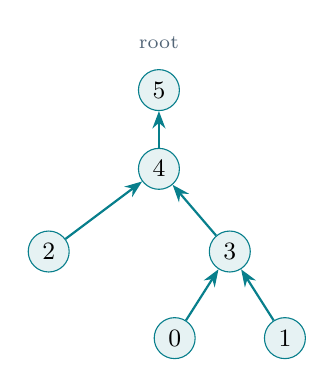
\begin{tikzpicture}
\node[vertex] (n5) at (0,2.5) {5};\node[vertex] (n4) at (0,1.5) {4};
\node[vertex] (n2) at (-1.4,.45) {2};\node[vertex] (n3) at (.9,.45) {3};
\node[vertex] (n0) at (.2,-.65) {0};\node[vertex] (n1) at (1.6,-.65) {1};
\draw[arr] (n4)--(n5);\draw[arr] (n2)--(n4);\draw[arr] (n3)--(n4);\draw[arr] (n0)--(n3);\draw[arr] (n1)--(n3);
\node[font=\scriptsize,text=Slate] at (0,3.1) {root};
\end{tikzpicture}
\par\small Illustrative parent array: $[3,3,4,4,5,6]$.\\Sentinel $6$ denotes a root.
\column{.54\textwidth}
\textbf{The preprocessing tree}
\begin{itemize}\setlength\itemsep{6pt}
\item SuperLU normally builds the column etree of the structural $(AP_c)^T(AP_c)$.
\item No numerical normal equations are solved.
\item A child-before-parent postorder groups complete subtrees contiguously.
\item Small subtrees can become relaxed supernodes.
\end{itemize}
\vspace{.2cm}\small One postorder here is $[2,0,1,3,4,5]$.
\end{columns}
\takeaway{The tree is structural guidance. For general LU, numerical pivoting still affects the actual factor structure.}
\end{frame}

% Slide 15 -------------------------------------------------------------
\begin{frame}{DFS reach finds which previous factor columns can contribute}
\begin{columns}[c,onlytextwidth]
\column{.53\textwidth}
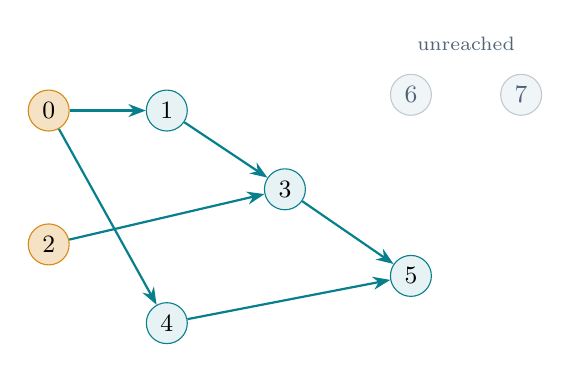
\begin{tikzpicture}
\node[vertex,fill=Amber!25,draw=Amber] (n0) at (0,1.8) {0};
\node[vertex] (n1) at (1.5,1.8) {1};
\node[vertex,fill=Amber!25,draw=Amber] (n2) at (0,.1) {2};
\node[vertex] (n3) at (3,.8) {3};
\node[vertex] (n4) at (1.5,-.9) {4};\node[vertex] (n5) at (4.6,-.3) {5};
\node[faint] (n6) at (4.6,2) {6};\node[faint] (n7) at (6,2) {7};
\draw[arr] (n0)--(n1);\draw[arr] (n0)--(n4);\draw[arr] (n1)--(n3);
\draw[arr] (n2)--(n3);\draw[arr] (n3)--(n5);\draw[arr] (n4)--(n5);
\node[font=\scriptsize,text=Slate] at (5.3,2.65) {unreached};
\end{tikzpicture}
\column{.43\textwidth}
\textbf{Scalar triangular-update illustration}
\begin{itemize}\setlength\itemsep{5pt}
\item An edge $j\to i$ represents a nonzero $l_{ij}$.
\item Start from sparse input support: nodes 0 and 2.
\item Reach follows dependencies; update in topological order.
\item Nodes 6 and 7 need no update in this example.
\end{itemize}
\small SuperLU groups reached contributions into supernodal segments and accounts for pivoted row indices.
\end{columns}
\takeaway{SuperLU's symbolic DFS is interleaved with numerical factorization. Our graph-envelope preprocessing is a simpler teaching substitute.}
\end{frame}

% Slide 16 -------------------------------------------------------------
\begin{frame}{A supernode shares row indices across consecutive columns}
\begin{columns}[c,onlytextwidth]
\column{.44\textwidth}\centering
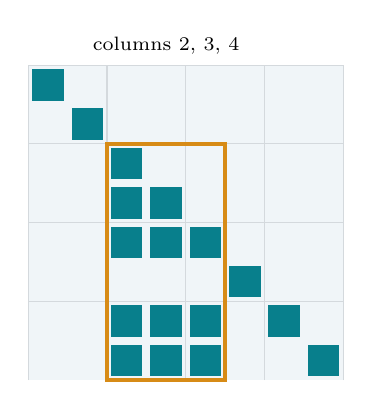
\begin{tikzpicture}[x=.5cm,y=.5cm]
\fill[Mist] (0,0) rectangle (8,-8);\draw[Slate!25] (0,0) grid (8,-8);
\foreach \r/\c in {0/0,1/1,2/2,3/2,3/3,4/2,4/3,4/4,5/5,6/2,6/3,6/4,6/6,7/2,7/3,7/4,7/7}
 {\fill[Teal] (\c+.1,-\r-.1) rectangle (\c+.9,-\r-.9);}
\draw[Amber,line width=1.2pt] (2,-2) rectangle (5,-8);
\node[font=\scriptsize] at (3.5,.5) {columns 2, 3, 4};
\end{tikzpicture}
\column{.10\textwidth}\centering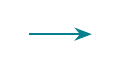
\begin{tikzpicture}\draw[arr] (0,0)--(.8,0);\end{tikzpicture}
\column{.42\textwidth}\centering
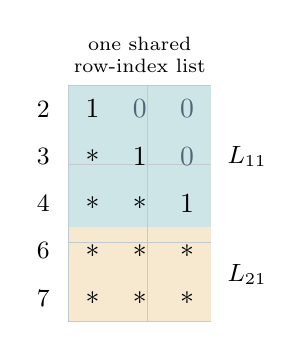
\begin{tikzpicture}[x=.6cm,y=.6cm]
\fill[Teal!20] (0,0) rectangle (3,-3);\fill[Amber!20] (0,-3) rectangle (3,-5);
\draw[Slate!35] (0,0) grid (3,-5);
\foreach \r/\label in {0/2,1/3,2/4,3/6,4/7}
 {\node[anchor=east,font=\small] at (-.2,-\r-.5) {\label};}
\foreach \r in {0,1,2}{\foreach \c in {0,1,2}{
 \ifnum\r=\c \node at (\c+.5,-\r-.5) {$1$};
 \else\ifnum\r>\c \node at (\c+.5,-\r-.5) {$*$};
 \else \node[text=Slate] at (\c+.5,-\r-.5) {$0$};\fi\fi}}
\foreach \r in {3,4}{\foreach \c in {0,1,2}{\node at (\c+.5,-\r-.5) {$*$};}}
\node[anchor=west,font=\small] at (3.15,-1.5) {$L_{11}$};\node[anchor=west,font=\small] at (3.15,-4) {$L_{21}$};
\node[font=\scriptsize,align=center] at (1.5,.65) {one shared\\row-index list};
\end{tikzpicture}
\end{columns}
\takeaway{The common rows below the diagonal block are 6 and 7. Packed dense blocks can store zeros; their triangular structure still matters. SuperLU forms supernodes during factorization.}
\end{frame}

% Slide 17 -------------------------------------------------------------
\begin{frame}{Our Python panels perform a genuine block Schur update}
\begin{columns}[c,onlytextwidth]
\column{.39\textwidth}\centering
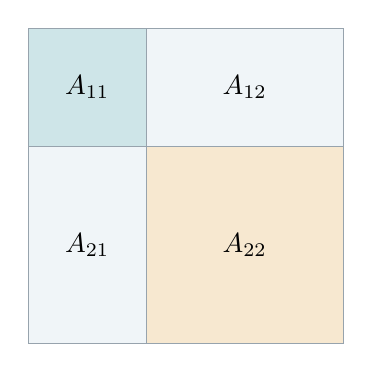
\begin{tikzpicture}
\fill[Teal!20] (0,0) rectangle (1.5,-1.5);
\fill[Mist] (1.5,0) rectangle (4,-1.5);\fill[Mist] (0,-1.5) rectangle (1.5,-4);
\fill[Amber!20] (1.5,-1.5) rectangle (4,-4);
\draw[Slate!60] (0,0) rectangle (4,-4);\draw[Slate!60] (1.5,0)--(1.5,-4);\draw[Slate!60] (0,-1.5)--(4,-1.5);
\node at (.75,-.75) {$A_{11}$};\node at (2.75,-.75) {$A_{12}$};
\node at (.75,-2.75) {$A_{21}$};\node at (2.75,-2.75) {$A_{22}$};
\end{tikzpicture}
\column{.57\textwidth}
\textbf{After accounting for panel row swaps:}
\begin{align*}
 A_{11} &= L_{11}U_{11},\\
 L_{11}U_{12} &= A_{12},\\
 L_{21}U_{11} &= A_{21},\\
 A_{22}^{\mathrm{new}} &= A_{22}-L_{21}U_{12}.
\end{align*}
\small The code computes $L_{21}$ while factoring panel columns, delays trailing updates, solves for $U_{12}$, then updates touched trailing positions.
\end{columns}
\takeaway{Block organization exposes dense arithmetic. Native optimized solvers use tuned kernels; this Python code keeps the operations explicit for study.}
\end{frame}

% Slide 18 -------------------------------------------------------------
\begin{frame}{Left-looking and right-looking schedule the same algebra differently}
\begin{columns}[c,onlytextwidth]
\column{.48\textwidth}\centering
\textbf{SuperLU: left-looking}\par\vspace{.15cm}
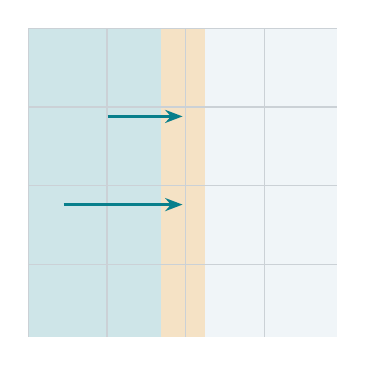
\begin{tikzpicture}[x=.56cm,y=.56cm]
\fill[Mist] (0,0) rectangle (7,-7);\fill[Teal!20] (0,0) rectangle (3,-7);
\fill[Amber!25] (3,0) rectangle (4,-7);\draw[Slate!30] (0,0) grid (7,-7);
\draw[arr,line width=1.2pt] (.8,-4)--(3.5,-4);\draw[arr,line width=1.2pt] (1.8,-2)--(3.5,-2);
\end{tikzpicture}
\par\small Gather earlier contributions into the current column/panel.
\column{.48\textwidth}\centering
\textbf{Our panel kernel: right-looking}\par\vspace{.15cm}
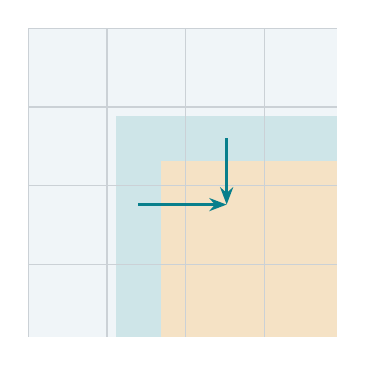
\begin{tikzpicture}[x=.56cm,y=.56cm]
\fill[Mist] (0,0) rectangle (7,-7);\fill[Teal!20] (2,-2) rectangle (7,-3);
\fill[Teal!20] (2,-3) rectangle (3,-7);\fill[Amber!25] (3,-3) rectangle (7,-7);
\draw[Slate!30] (0,0) grid (7,-7);\draw[arr,line width=1.2pt] (2.5,-4)--(4.5,-4);
\draw[arr,line width=1.2pt] (4.5,-2.5)--(4.5,-4);
\end{tikzpicture}
\par\small Push the finished panel's contribution into the trailing matrix.
\end{columns}
\takeaway{A similar stage diagram does not imply the same implementation. Scheduling changes workspace, locality, and sparse traversal.}
\end{frame}

% Slide 19 -------------------------------------------------------------
\begin{frame}{CSR stores values and column indices, row by row}
\begin{columns}[c,onlytextwidth]
\column{.36\textwidth}\centering
$A=$\numatrix{4\&0\&2\&0\\0\&3\&0\&0\\1\&0\&5\&6\\0\&0\&0\&7\\}{3/1,3/3,3/4}{}
\par\vspace{.3cm}\small Highlighted: row $i=2$\\(zero-based indexing).
\column{.61\textwidth}
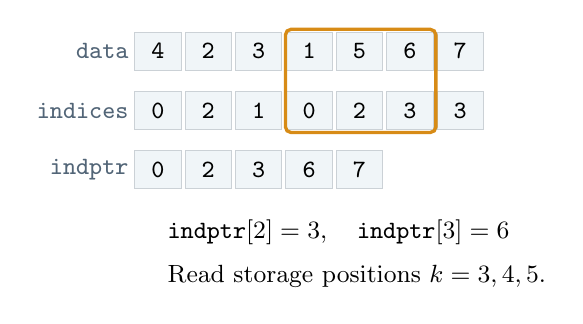
\begin{tikzpicture}
\arrayrow{1.3}{data}{4,2,3,1,5,6,7}
\arrayrow{.55}{indices}{0,2,1,0,2,3,3}
\arrayrow{-.2}{indptr}{0,2,3,6,7}
\draw[Amber,line width=1.2pt,rounded corners=2pt] (1.62,.27) rectangle (3.53,1.58);
\node[anchor=west,font=\small] at (0,-1.0) {$\texttt{indptr}[2]=3,\quad\texttt{indptr}[3]=6$};
\node[anchor=west,font=\small] at (0,-1.55) {Read storage positions $k=3,4,5$.};
\end{tikzpicture}
\end{columns}
\takeaway{$i$ is a matrix row, $k$ is a storage position, and $j=\texttt{indices}[k]$ is a matrix column.}
\end{frame}

% Slide 20 -------------------------------------------------------------
\begin{frame}{CSC groups the same entries by column}
\begin{columns}[c,onlytextwidth]
\column{.36\textwidth}\centering
$A=$\numatrix{4\&0\&2\&0\\0\&3\&0\&0\\1\&0\&5\&6\\0\&0\&0\&7\\}{1/3,3/3}{}
\par\vspace{.3cm}\small Highlighted: column $j=2$.
\column{.61\textwidth}
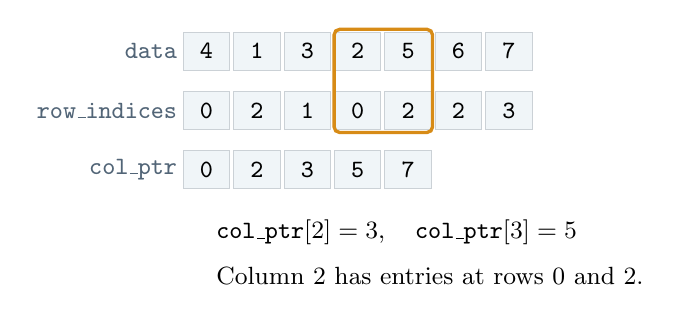
\begin{tikzpicture}
\arrayrow{1.3}{data}{4,1,3,2,5,6,7}
\arrayrow{.55}{row\_indices}{0,2,1,0,2,2,3}
\arrayrow{-.2}{col\_ptr}{0,2,3,5,7}
\draw[Amber,line width=1.2pt,rounded corners=2pt] (1.62,.27) rectangle (2.87,1.58);
\node[anchor=west,font=\small] at (0,-1.0) {$\texttt{col\_ptr}[2]=3,\quad\texttt{col\_ptr}[3]=5$};
\node[anchor=west,font=\small] at (0,-1.55) {Column 2 has entries at rows 0 and 2.};
\end{tikzpicture}
\end{columns}
\takeaway{SuperLU processes CSC input. The Python implementation provides a CSC view for structure and diagnostics, while dictionary rows carry the numerical working matrix.}
\end{frame}

% Slide 21 -------------------------------------------------------------
\begin{frame}{The code separates analysis, factors, and solves}
\centering
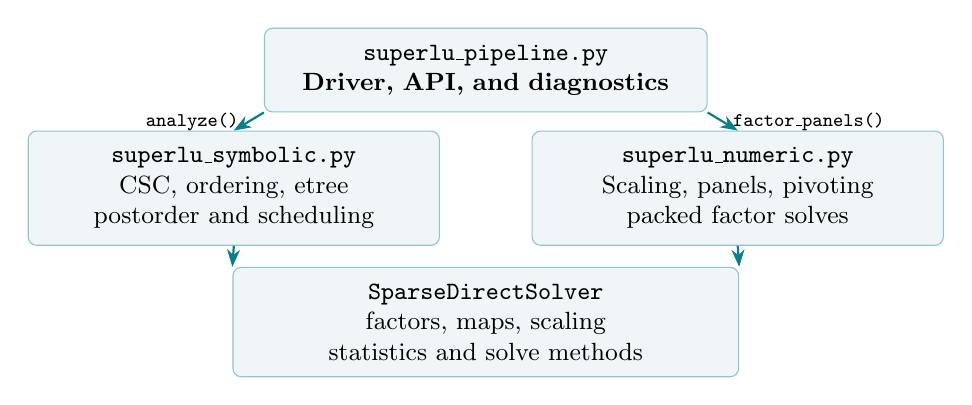
\begin{tikzpicture}
\node[flow,text width=5.2cm] (driver) at (6,1.3) {\texttt{superlu\_pipeline.py}\\\textbf{Driver, API, and diagnostics}};
\node[flow,text width=4.8cm] (symbolic) at (2.8,-.2) {\texttt{superlu\_symbolic.py}\\CSC, ordering, etree\\postorder and scheduling};
\node[flow,text width=4.8cm] (numeric) at (9.2,-.2) {\texttt{superlu\_numeric.py}\\Scaling, panels, pivoting\\packed factor solves};
\node[flow,text width=6cm] (solver) at (6,-1.9) {\texttt{SparseDirectSolver}\\factors, maps, scaling\\statistics and solve methods};
\draw[arr] (driver.south west)--node[left,font=\scriptsize]{\texttt{analyze()}}(symbolic.north);
\draw[arr] (driver.south east)--node[right,font=\scriptsize]{\texttt{factor\_panels()}}(numeric.north);
\draw[arr] (symbolic.south)--(solver.north west);
\draw[arr] (numeric.south)--(solver.north east);
\end{tikzpicture}\par\vspace{.25cm}
\small Supporting code: \texttt{sparse\_solver.py} supplies CSR and Poisson construction; \texttt{sparse\_lu.py} provides a compact scalar LU baseline.
\takeaway{A structural plan is reusable across value changes. Numerical factors are reusable across RHS changes. The driver owns both lifecycles.}
\end{frame}

% Slide 22 -------------------------------------------------------------
\begin{frame}[fragile]{The public API follows analyze, factorize, solve, and assess}
\begin{columns}[T,onlytextwidth]
\column{.62\textwidth}
\begin{lstlisting}
from sparse_learning.sparse_solver import poisson_2d
from sparse_learning.superlu_symbolic import analyze
from sparse_learning.superlu_pipeline import factorize

A = poisson_2d(8)
b = A.matvec([1.0] * 64)
plan = analyze(A, ordering="minimum_degree")
solver = factorize(A, analysis=plan)
x = solver.solve(b)
report = solver.refine(b, x)

print(report.componentwise_backward_error)
\end{lstlisting}
\column{.34\textwidth}
\small\textbf{Objects you can inspect}
\begin{itemize}\setlength\itemsep{6pt}
\item \texttt{plan}: ordering, etree, patterns, panels.
\item \texttt{solver}: $L,U$, permutations, scales, supernodes.
\item \texttt{report}: solution, residual, error and condition estimates.
\end{itemize}
\end{columns}
\takeaway{Calling \texttt{factorize(A)} directly performs analysis automatically. Passing a plan makes structural reuse explicit.}
\end{frame}

% Slide 23 -------------------------------------------------------------
\begin{frame}[fragile]{The symbolic module turns sparsity into an execution plan}
\begin{columns}[T,onlytextwidth]
\column{.60\textwidth}
\begin{lstlisting}
graph = column_graph(A)
order = minimum_degree(graph)
etree, columns = symbolic_cholesky(
    permute_graph(graph, order))

post = tree_postorder(etree)
order = [order[j] for j in post]
etree, columns = symbolic_cholesky(
    permute_graph(graph, order))

relaxed = relaxed_supernodes(etree, relax)
panels = panel_schedule(n, panel_size, relaxed)
\end{lstlisting}
\small Excerpt of the default minimum-degree / postorder path in \texttt{analyze()}.
\column{.36\textwidth}
\small\textbf{Stored in \texttt{SymbolicAnalysis}}
\begin{itemize}\setlength\itemsep{5pt}
\item Canonical input pattern.
\item New-to-old column order.
\item Etree and structural column sets.
\item Strict / relaxed groups and panel ranges.
\end{itemize}
\small Pattern checks prevent reuse after structural changes.
\end{columns}
\takeaway{This implementation models the structural $A^TA$ envelope. Its column sets guide scheduling rather than preallocating exact pivoted LU patterns.}
\end{frame}

% Slide 24 -------------------------------------------------------------
\begin{frame}{The numerical module maintains a sparse Schur complement}
\begin{columns}[T,onlytextwidth]
\column{.44\textwidth}
\textbf{State in \texttt{factor\_panels()}}
\small\begin{itemize}\setlength\itemsep{6pt}
\item \texttt{work}: completed $U$ rows and the active Schur complement.
\item \texttt{lower}: previously computed multipliers.
\item \texttt{rows / row\_position}: equation permutation and its inverse.
\item \texttt{stats}: swaps, fill insertions, work size.
\end{itemize}
\column{.52\textwidth}
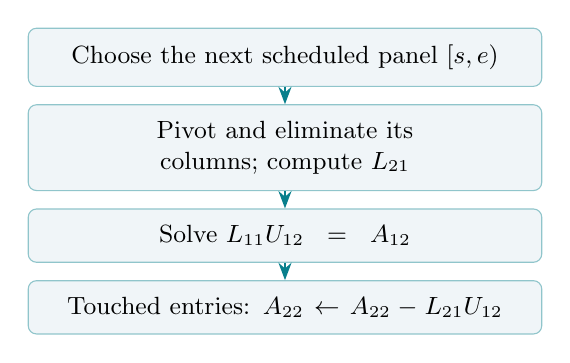
\begin{tikzpicture}[node distance=.22cm]
\node[flow,text width=6.1cm,font=\small] (p) {Choose the next scheduled panel $[s,e)$};
\node[flow,text width=6.1cm,font=\small,below=of p] (pivot) {Pivot and eliminate its columns; compute $L_{21}$};
\node[flow,text width=6.1cm,font=\small,below=of pivot] (trsv) {Solve $L_{11}U_{12}=A_{12}$};
\node[flow,text width=6.1cm,font=\small,below=of trsv] (update) {Touched entries: $A_{22}\leftarrow A_{22}-L_{21}U_{12}$};
\draw[arr] (p)--(pivot);\draw[arr] (pivot)--(trsv);\draw[arr] (trsv)--(update);
\end{tikzpicture}
\end{columns}
\takeaway{The numerical state grows when fill appears. Exact zeros are removed; small nonzero entries are retained. Row swaps also move existing multipliers.}
\end{frame}

% Slide 25 -------------------------------------------------------------
\begin{frame}[fragile]{The solve method applies maps around a packed triangular solve}
\begin{columns}[T,onlytextwidth]
\column{.60\textwidth}
\begin{lstlisting}
q, p = self.analysis.col_order, self.row_order
rhs = [self.scaling.row[i] * b[i] for i in p]
z = triangular_solve(self.supernodes, rhs)
x = [0.0] * self.n
for k, old in enumerate(q):
    x[old] = self.scaling.column[old] * z[k]
\end{lstlisting}
\small Normal-solve path from \texttt{SparseDirectSolver.solve()}.
\vspace{.25cm}
\textbf{Packed factor storage}
\small\begin{itemize}\setlength\itemsep{5pt}
\item Each \texttt{Supernode} holds $L_{11},U_{11},L_{21},U_{12}$ and shared indices.
\item \texttt{U\_csc} exposes an additional CSC view for inspection.
\end{itemize}
\column{.36\textwidth}
\textbf{Transpose solve $A^Tx=b$}
\begin{align*}
\widehat b &= P_c^TCb,\\
U^Tv &= \widehat b,\\
L^Tz &= v,\\
x &= RP_r^Tz.
\end{align*}
\small Transpose solves also support inverse-norm estimation.
\end{columns}
\takeaway{Permutations and scaling are part of the solve algorithm. The factor-space solution must be mapped back to the original variable order.}
\end{frame}

% Slide 26 -------------------------------------------------------------
\begin{frame}{Refinement uses residuals to correct the computed solution}
\begin{columns}[c,onlytextwidth]
\column{.47\textwidth}\centering
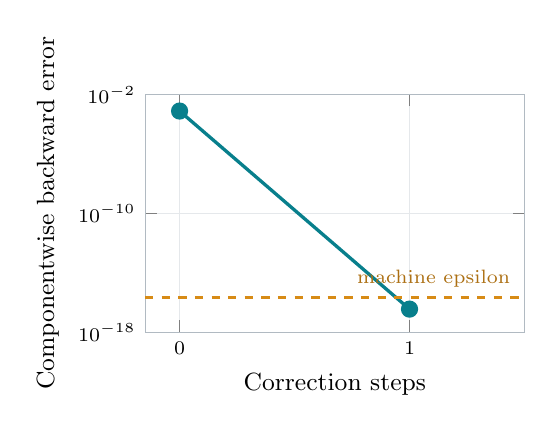
\begin{tikzpicture}
\begin{semilogyaxis}[
 width=6.4cm,height=4.6cm,
 xlabel={Correction steps},ylabel={Componentwise backward error},
 xmin=-0.15,xmax=1.5,xtick={0,1},
 ymin=1e-18,ymax=1e-2,
 grid=major,grid style={Slate!15},
 tick label style={font=\scriptsize},label style={font=\small},
 axis line style={Slate!45},
]
\addplot[Teal,very thick,mark=*,mark size=2.5pt] coordinates {(0,7.836562081731e-04) (1,3.629965303959e-17)};
\addplot[Amber,dashed,thick,domain=-0.15:1.5] {2.220446049250313e-16};
\node[anchor=south east,font=\scriptsize,text=Amber!80!black]
 at (axis cs:1.48,2.220446049250313e-16) {machine epsilon};
\end{semilogyaxis}
\end{tikzpicture}

\par\scriptsize Actual scaled $8\times8$ grid; initial solution perturbed by $10^{-3}$.\\80-digit residual arithmetic, float64 factors.
\column{.49\textwidth}
\begin{align*}
 r &= b-Ax,\\
 A\,\delta x &= r \quad\text{(reuse LU)},\\
 x &\leftarrow x+\delta x.
\end{align*}
\small\textbf{Diagnostics answer different questions}
\[
 \mathrm{berr}=\max_i\frac{|r_i|}{(|A||x|+|b|)_i}
\]
\[
 \mathrm{rcond}_1\approx\frac{1}{\|A\|_1\|A^{-1}\|_1}.
\]
\small Condition and forward-error estimates use normal and transpose solves without forming an inverse.
\end{columns}
\takeaway{A small residual alone does not guarantee small solution error. Conditioning connects those two quantities.}
\end{frame}

% Slide 27 -------------------------------------------------------------
\begin{frame}{Reuse depends on what changed}
\centering
\begin{tabular}{@{}p{3.5cm}p{4.9cm}p{4.9cm}@{}}
\toprule
\textbf{Change} & \textbf{What can be reused?} & \textbf{What must run again?}\\
\midrule
Only $b$ changes & Scaling, order, symbolic plan, $L,U$ & Triangular solves; optional refinement\\[9pt]
Values of $A$ change; pattern stays & Column order, etree, scheduling plan & Numerical factorization; scaling can be recomputed\\[9pt]
Sparsity pattern changes & Existing plan needs revalidation & Ordering and symbolic analysis, then factorization\\
\bottomrule
\end{tabular}
\vspace{.35cm}
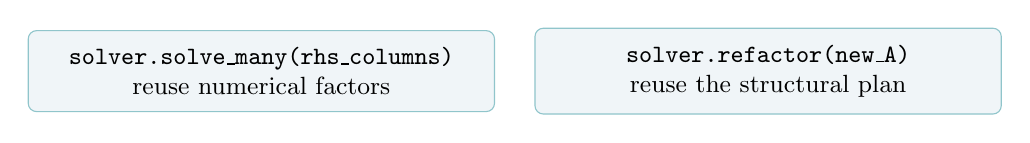
\begin{tikzpicture}
\node[flow,text width=5.5cm] (same) {\texttt{solver.solve\_many(rhs\_columns)}\\reuse numerical factors};
\node[flow,text width=5.5cm,right=.5cm of same] {\texttt{solver.refactor(new\_A)}\\reuse the structural plan};
\end{tikzpicture}
\takeaway{An old pivot sequence is only a preference. The Python refactorization checks each reused pivot against the current threshold.}
\end{frame}

% Slide 28 -------------------------------------------------------------
\begin{frame}{Verification checks algebra, numerical accuracy, and reuse}
\begin{columns}[T,onlytextwidth]
\column{.47\textwidth}
\textbf{Stage and integration checks}
\small\begin{itemize}\setlength\itemsep{6pt}
\item Factor identity $P_rRACP_c=LU$.
\item Initial and late pivoting; fill creation.
\item Normal / transpose solves and scaling modes.
\item Supernode blocks and panel widths.
\item Multiple RHS, same-pattern reuse, singular inputs.
\end{itemize}
\column{.49\textwidth}
\textbf{Independent SuperLU comparison}
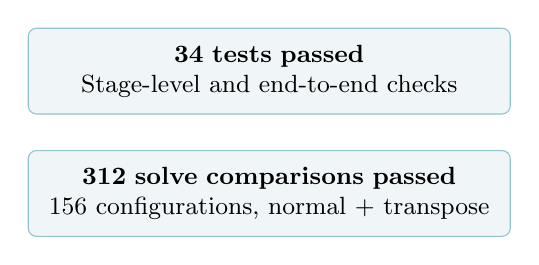
\begin{tikzpicture}
\node[flow,text width=5.7cm] (checks) {\textbf{34 tests passed}\\Stage-level and end-to-end checks};
\node[flow,text width=5.7cm,below=.45cm of checks] {\textbf{312 solve comparisons passed}\\156 configurations, normal + transpose};
\end{tikzpicture}\par\vspace{.2cm}
\small Largest relative solution difference: $2.9\times10^{-15}$. Checks use SciPy's actual SuperLU implementation as an independent reference.
\end{columns}
\takeaway{Tests establish behavior on the checked matrices; they do not establish production performance or coverage of every matrix class.}
\end{frame}

% Slide 29 -------------------------------------------------------------
\begin{frame}{The actual SuperLU loop interleaves symbolic and numeric work}
\begin{columns}[T,onlytextwidth]
\column{.37\textwidth}
\textbf{At the panel level}\par\vspace{.25cm}
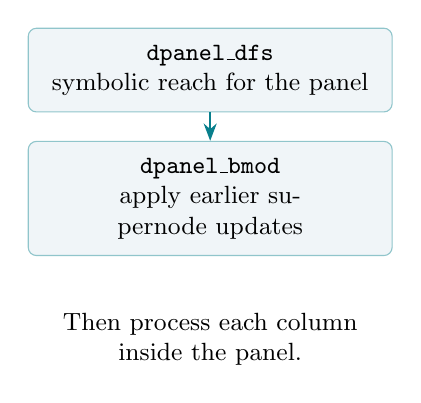
\begin{tikzpicture}[node distance=.36cm]
\node[flow,text width=4.2cm] (dfs) {\texttt{dpanel\_dfs}\\symbolic reach for the panel};
\node[flow,text width=4.2cm,below=of dfs] (bmod) {\texttt{dpanel\_bmod}\\apply earlier supernode updates};
\draw[arr] (dfs)--(bmod);
\node[font=\small,align=center,text width=4.2cm,below=.6cm of bmod] {Then process each column\\inside the panel.};
\end{tikzpicture}
\column{.59\textwidth}
\textbf{For each column}\par\vspace{.1cm}
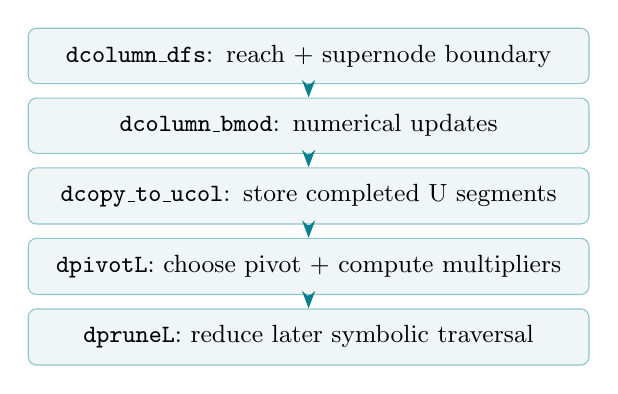
\begin{tikzpicture}[node distance=.17cm]
\node[flow,text width=6.7cm,minimum height=.48cm,font=\small] (cdfs) {\texttt{dcolumn\_dfs}: reach + supernode boundary};
\node[flow,text width=6.7cm,minimum height=.48cm,font=\small,below=of cdfs] (cbmod) {\texttt{dcolumn\_bmod}: numerical updates};
\node[flow,text width=6.7cm,minimum height=.48cm,font=\small,below=of cbmod] (copy) {\texttt{dcopy\_to\_ucol}: store completed U segments};
\node[flow,text width=6.7cm,minimum height=.48cm,font=\small,below=of copy] (pivot) {\texttt{dpivotL}: choose pivot + compute multipliers};
\node[flow,text width=6.7cm,minimum height=.48cm,font=\small,below=of pivot] (prune) {\texttt{dpruneL}: reduce later symbolic traversal};
\draw[arr] (cdfs)--(cbmod);\draw[arr] (cbmod)--(copy);\draw[arr] (copy)--(pivot);\draw[arr] (pivot)--(prune);
\end{tikzpicture}
\end{columns}
\takeaway{Read the main loop in \texttt{dgstrf.c}, then follow these calls individually. Relaxed-supernode processing provides a separate path in that loop.}
\end{frame}

% Slide 30 -------------------------------------------------------------
\begin{frame}{The teaching pipeline and SuperLU share stages, not all kernels}
\small
\begin{tabular}{@{}p{2.5cm}p{5.65cm}p{5.35cm}@{}}
\toprule
\textbf{Aspect} & \textbf{This Python implementation} & \textbf{Local SuperLU source}\\
\midrule
Input / work & CSR input, CSC view, mutable dictionary work & CSC input, specialized sparse arrays and panel workspace\\[5pt]
Ordering & Exact minimum degree on structural $A^TA$ & COLAMD, minimum-degree variants, other options\\[5pt]
Symbolic work & Explicit graph fill / etree envelope & Panel and column DFS, reach segments, pruning\\[5pt]
Numerical kernel & Blocked right-looking panels & Left-looking supernodal updates\\[5pt]
Supernodes & Detected and packed after numerical LU; used by solves & Formed during factorization, including relaxed groups\\[5pt]
Shared roles & Scaling, permutations, pivot tests, solves, refinement, reuse & Corresponding driver stages\\
\bottomrule
\end{tabular}
\takeaway{Use the Python implementation to inspect the algebra. Use the source call graph to learn SuperLU's specific storage and traversal strategy.}
\end{frame}

% Slide 31 -------------------------------------------------------------
\begin{frame}[fragile]{Run the code and connect each stage to its source}
\begin{columns}[T,onlytextwidth]
\column{.57\textwidth}
\textbf{Trace a complete factorization}
\begin{lstlisting}[language=bash]
python3 sparse_learning/superlu_pipeline.py \
    --grid 8 --trace

python3 sparse_learning/superlu_pipeline.py \
    --example scaled --grid 8

python3 -m unittest discover -s sparse_learning
\end{lstlisting}
\small The solver and deck figure generator require only the Python standard library. Independent reference validation additionally uses NumPy and SciPy.
\column{.39\textwidth}
\textbf{SuperLU source entry points}
\small\begin{itemize}\setlength\itemsep{6pt}
\item \texttt{dgssv.c}: basic driver.
\item \texttt{sp\_preorder.c}: column maps and etree.
\item \texttt{dgstrf.c}: panel / column factorization loop.
\item \texttt{dgstrs.c}: factor solves.
\item \texttt{dgssvx.c}: expert driver and diagnostics.
\end{itemize}
\end{columns}
\takeaway{Follow the same progression in mathematics and code: maps, structure, numerical factors, triangular solves, and accuracy checks.}
\end{frame}

\end{document}
